%\documentclass[twoside,openright,a4paper,11pt]{book}
%
%
\usepackage[utf8]{inputenc}
\usepackage[francais]{babel}
\usepackage[T1]{fontenc}

\addto\captionsfrench{\def\tablename{\textsc{Tableau}}}% pour avoir TABLEAU et pas TABLE dans les légendes des tableaux

%%%%%%% MISE EN PAGES %%%%%%
\usepackage{geometry}
\geometry{outer=2cm,inner=3cm,top=3cm}

\setcounter{tocdepth}{3}     % Dans la table des matieres
\setcounter{secnumdepth}{3}  % Avec un numero.
\usepackage{setspace}

\usepackage{fancyhdr}	% marge en haut et en bas
\pagestyle{fancy}

\fancyhead{}	% vide l'entête
\fancyfoot{} % vide le pied~de~page

\fancyhead[RO]{\leftmark}
\fancyhead[LE]{\rightmark}
\fancyfoot[C]{\thepage}	% numéro de page en bas au centre

\renewcommand{\headrulewidth}{0.4pt} % épaisseur du trait en haut
\renewcommand{\footrulewidth}{0.4pt} % épaisseur du trait en bas

\fancypagestyle{mypagestyle}{%
    \fancyhead{}	
    \fancyfoot{} 
    \fancyfoot[C]{\thepage}
    \renewcommand{\headrulewidth}{0.4pt} 
	\renewcommand{\footrulewidth}{0.4pt} 
}

\fancypagestyle{couvertureAbstract}{%
    \fancyhead{}	
    \fancyfoot{} 
    \fancyfoot[C]{}
	\renewcommand{\headrulewidth}{0pt} 
	\renewcommand{\footrulewidth}{0pt} 
}
%
\usepackage{layout}
\usepackage{tocbibind} % include tableofcontent in itself

%%%%%% PAGE DE GARDE %%%%%%

\geometry{outer=2cm,inner=3cm,top=3cm}
\usepackage[scaled]{helvet} % font used on cover (Helvetica)
\usepackage{eso-pic} % to set background picture
\usepackage{multicol} % for back cover (abstracts)
\usepackage{graphicx} % to include logos
\usepackage{tikz} % to compose background picture

% Colors (extracted from SPI's template)
\definecolor{boxcolor1}{rgb}{0.91373,0.92941,0.87451}
\definecolor{boxcolor2}{rgb}{0.94902,0.93333,0.91373}
\definecolor{boxcolor3}{rgb}{0.76078,0.87843,0.17647}
\definecolor{headercolor}{rgb}{0.94118,0.30980,0.17255}
\definecolor{namecolor}{rgb}{1.0,0.4,0.0}
\definecolor{titlecolor}{rgb}{0.19216,0.51765,0.60784}
% Also used: gray, teal (predefined by xcolor package, usually loaded by document class)

% Cover environment, to keep changes local
\newenvironment{cover}{%
  \fontfamily{phv}\selectfont % Select Helvetica font
  \pagestyle{empty} % No page number
}{
  \addtocounter{page}{-1}
  \cleardoublepage
}

% Macro for background common to front and back
\newcommand{\tikzBG}{%
  \path (0,0) rectangle (1,1);
  %TODO: You should adjust the bottom height of the following rectangle to fit your abstract's length
  \path [fill=boxcolor1] (.0571,.11) rectangle (.481,.963); 
  \path [fill=boxcolor2] (.4333,.697) rectangle (.9048,.7475);
  \path [fill=boxcolor2] (.4333,.7811) rectangle (.9048,.8316);
  \path [fill=boxcolor2] (.4333,.8687) rectangle (.9048,.9192);
  \path [fill=boxcolor3] (.0571,.7879) rectangle (.5762,.8316);
  \node[inner sep=0pt] at (0.2285,0.8788) [above left] {%
    
\includegraphics[height=.0707\paperheight,keepaspectratio]{./figures/logo/logo_unb.png}};
  \node[inner sep=0pt] at (0.6667,0.8788) [above right] {%
    
\includegraphics[height=.0808\paperheight,keepaspectratio]{./figures/logo/logo_ecn_color.png}};
  \node at (.0571,.8316) [above right,color=headercolor] {%
    \fontsize{29}{35}\selectfont\bfseries Th\`ese de Doctorat};
}

% Macro for repeated information (to avoid insconsistency)
%TODO: fill in with no formatting but desired case
\newcommand{\firstName}{Jean-Rémy}
\newcommand{\surname}{Gloaguen}
\newcommand{\thesisTitle}{Estimation du niveau sonore de sources d'intérêts au sein de mixtures sonores urbaines : application au trafic routier}

%%%%%%% SYMBOLES %%%%%
\usepackage{tipa}	% pour avoir l'accent concave
\usepackage{lmodern}	% pour les guillemets
\usepackage{gensymb}	% pour les degrés
\usepackage{enumitem}	% pour changer le symbole de l'item (\begin{itemize}[label=$\bullet$])

%%%%%%% EQUATION %%%%%%
\usepackage{amssymb}
\usepackage{amsmath}
\usepackage{fancybox}
\usepackage{xfrac}	% fraction de type "1/4"
\usepackage{cases}	% système équation
\usepackage[overload]{empheq}
\usepackage{bm}		% pour mettre en gras .
\usepackage{units} 	% x/y barre latérale pour les fractions
%
%%%%%%% FIGURE %%%%%%
\usepackage{subfigure}	% utiliser subfigure
\usepackage{float}	% utiliser H dans les figures
%
%%%%%% TABLEAUX %%%%%%
\usepackage{array,multirow,makecell}
%\addto\captionsfrench{\def\tablename{\textsc{Tableau}}}% pour avoir TABLEAU et pas TABLE dans les légendes des tableaux
\usepackage{colortbl} % pour avoir des lignes colorées dans les tableau
%\usepackage{slashbox} % pour les \backslashbox
%\usepackage{subcaption}
\usepackage{hhline}	% pour les lignes horizontales 
\usepackage{tabularx} % permet itemize dans les cellules
\usepackage{booktabs}
\usepackage{longtable}	% pour les tableaux longs

\newcolumntype{L}[1]{>{\raggedright\let\newline\\\arraybackslash\hspace{0pt}}m{#1}}
\newcolumntype{C}[1]{>{\centering\let\newline\\\arraybackslash\hspace{0pt}}m{#1}}
\newcolumntype{R}[1]{>{\raggedleft\let\newline\\\arraybackslash\hspace{0pt}}m{#1}}

%%%%% ALGORITHME %%%%%
\usepackage{algorithm}
\usepackage{algorithmic}

%%%%% BIBLIO %%%%%
\usepackage[fixlanguage]{babelbib}
\selectbiblanguage{french}
\usepackage{breakcites}	% pour couper les références en bout de ligne

%%%%% APPENDICES %%%%%%%
\usepackage[toc,page]{appendix}

%%%%%%%%%%%%%%%%%%%%%
\usepackage{url}	% gérer les adresses www.
\linespread{1.2}	% interligne

\cleardoublepage
%
%
%\begin{document}

\chapter{Création de corpus de mixtures sonores urbaines}
\label{chap:corpusSonore}

La méthode de la NMF a été retenue comme estimateur afin d'obtenir les niveaux sonores du trafic routier. Toutefois, nous choisissons de ne pas l'appliquer directement sur des enregistrements audio réalisés en ville. En effet, le trafic sonore y est alors mélangé à d'autres sources sonores. Son niveau sonore exact est alors inconnu. Il n'est donc pas possible de comparer l'estimation fournie par la méthode NMF avec une valeur de référence et ainsi évaluer ses performances et sa justesse. L'approche choisie est ici d'appliquer cet estimateur sur des scènes sonores urbaines simulées où la contribution du trafic routier sera connue avec précision et où les estimations des niveaux sonores pourront être comparées aux niveaux exacts. Cette choix soulève plusieurs questions : comment composer des mixtures sonores urbaines aussi réalistes que des enregistrements sonores ? Comment s'assurer que les corpus de sons sur lesquels sont appliqués les algorithmes permettent de tester les limites des estimateurs ?
Il en effet nécessaire de s'attarder sur la création des mixtures sonores urbaines et sur la qualité de leur composition afin que les choix architecturaux effectués à la lumière des expérimentations soient d'intérêts.

La création d'environnements sonores urbains réalistes dépasse la question de l'estimation du niveau sonore du trafic.L'intérêt d'utiliser des scènes sonores issus d'un processus de simulation est de permettre un meilleur contrôle sur leur composition où la présence des différentes classes de son, ainsi que leur niveau sonore, est alors définie par l'utilisateur en fonction de ses besoins.
Leur utilisation trouve un intérêt dans le cadre des études perceptives des ESU. Leur utilisation a déjà été réalisée pour, par exemple, étudier l'agrément sonore à partir de scènes sonores recréées directement par les participants et estimer l'influence de la présence des sources sonores \cite{lafay_new_2014}, ce que ne permet pas l'écoute faite en ville \cite{adams_soundwalking_2008, liu2014effects} ou en laboratoire d'enregistrements audio \cite{guastavino2005ecological, cain2013development}.
Ces scènes sonores simulées peuvent également trouver un intérêt pour tester et développer des outils de traitement du signal \cite{Komatsu2016, geiger2015improving} où l'utilisation de scènes sonores simulées permet d'éviter l'étape d'annotation manuelle, qui peut être longue et fastidieuse.

Toutefois, si l'utilisation de scènes sonores simulées a de nombreux avantages, la question de leur validité écologique est importante. En effet, la réalisation de \textit{soundwalks} ou l'utilisation d'enregistrements sonore permettent de baser ces études sur des scènes sonores réelles et donc de mieux s'assurer que les outils sont bien adaptés à ces environnements.

En conséquence, il y a un intérêt certain à savoir simuler des environnements sonores urbains de façon à obtenir une complexité et un réalisme suffisant, c'est-à-dire assimilable à des enregistrements faits en ville. Cette tâche reste un défi qui n'a, pour l'instant, pas été relevé et n'est pas trivial puisque l'environnement sonore urbain est un milieu extrêmement variable à la fois temporellement (à un endroit donné, les sources sonores varient constamment) et spatialement (d'un quartier à un autre, les sources ne sont pas les mêmes).
Ce chapitre décrit notre méthode de création des corpus de scènes sonores urbaines simulées. Dans une première partie, plusieurs approches permettant de simuler de tels environnements sont résumées, puis l'outil retenu est présenté en détail. Les étapes menant à la création d'une base de données, appelé corpus élémentaire, et de deux corpus d'évaluation sont ensuite exposées. On présente enfin le test perceptif et les résultats obtenus démontrant le réalisme d'un des corpus.

\section{Création de scènes sonores : choix d'une méthode}

Dans une première partie, deux approches pour réaliser des scènes sonores urbaines sont présentés : l'auralisation et la simulation de scènes sonores.

\subsection{Auralisation d'ESU}

Une des premières approches possible pour restituer un ESU est d'utiliser les techniques d'auralisation \cite{forssen2009auralization}. Cette méthode vise à modéliser l'évolution temporelle d'un signal sonore $M_i(t)$ en un point $i$ en prenant en compte les différentes sources sonores présente $s_j(t)$ et l'environnement spatial $\delta_{ij}(t)$ et les effets qu'ils génèrent sur la propagation des sources sonores. Cette méthode équivaut à modéliser les équations \ref{eq:convolution_ESU} et \ref{eq:propagation}. En choisissant le type et le nombre de sources, l'environnement urbain, il est alors envisageable de déterminer en un point la contribution de chaque source sonore.
Pour cela, on réalise la convolution entre la réponse impulsionnelle d'une rue, obtenue soit par sa mesure soit par sa modélisation par un logiciel (CATT-acoustics, I-Simpa \dots), avec un signal sonore, enregistré dans des conditions d'anéchoïcité ou bien synthétisé. La restitution de l'ESU en un point donné et son évolution dans le temps peut alors être écoutées \cite{vorlander2007auralization}. Cette tâche reste toutefois complexe pour un tel environnement :

\begin{itemize}
\item La mesure de réponses impulsionnelles des rues \cite{picaut2005experimental} est une tâche complexe à réaliser puisqu'elle nécessite un dispositif expérimental conséquent qui doit être utilisé avec des conditions les plus neutres possibles (faible bruit de fond, conditions météorologiques neutres).
\item La modélisation numérique des rues est alors la voie la plus souvent choisie car elle offre plus de possibilité, mais cela nécessite tout de même de simplifier l'environnement (allure des façades, présence de petits mobiliers urbain) afin de limiter les temps de calculs.
\item Les effets de propagation du son en tenant en compte les phénomènes de diffusion, de réflexions dans un milieu urbain sont encore difficile à modéliser avec un rendu réaliste \cite{schissler2014high}.
\item La modélisation dynamique des sources sonores n'est modélisée que pour certaines sources sonores, comme le trafic routier ou ferroviaire, en utilisant des modèles dynamiques pour simuler leur déplacement. Ce sont alors des enregistrements audio qui permettent de modéliser les autres sources sonores, ce qui, si c'est une approche plus simple, est plus restreint en terme de contrôle par l'utilisateur. 
\ml{$testPerceptif_boxplotAmbianceCOLOR_EN$}
\end{itemize}

\cite{stienen2015auralization} résument ces différents aspects, les questions soulevées et les champs d'applications que permet l'auralisation des environnements sonore urbains.
Si cette tâche reste complexe, il existe tout de même quelques outils comme le logiciel \textit{MithraSON} du CSTB qui propose de générer des ESU \footnote{extrait sonore \url{https://www.youtube.com/watch?v=ACCV2mi81j8}}. À partir d'un quartier modélisé, les sources sonores liées au trafic sont générés en temps réel à partir d'une synthèse granulaire et à l'aide d'un modèle dynamique de trafic. L'ensemble des autres sources sonores (voix, oiseaux, cloche \dots) est basé sur des enregistrements audio qui sont ensuite intégré à l'ESU. La propagation des signaux est générée à l'aide d'une méthode de tirs de rayons.
Même si les résultats permettent une forte immersion, grâce à la spatialisation du son par l'écoute binaurale, cette méthode reste complexe à implémenter et nécessitent des ressources numériques importantes.

\subsection{Simulateur de scènes sonores}

Une autre approche pour simuler les environnements sonores urbains consiste à considérer l'ESU selon la description de R. Schafer, dans sa définition du paysage sonore \cite{schafer1977tuning} : une combinaison de bruits de fond (ou texture  sonore) et d'évènements sonores (ou objets sonores) qui, par un processus additif, permet alors de créer des mixtures sonores formant l'ESU \ml{je ne pense pas que sachafer dise cela, regarde plutot nelken skeleton of events on a bed of textures}. La catégorie bruit de fond inclut des sons plus longs (plusieurs minutes) dont les propriétés acoustiques ne varient pas dans le temps comme le bruit généré par un trafic continu, le chant des oiseaux dans un parc ou les voies des enfants dans une cours de récréation.
La catégorie \textit{évènement} équivaut à des sons brefs (de 1 à plusieurs secondes) qui émergent du bruit de fond pour être perçu individuellement par un auditeur (un voiture qui passe, des bruits de pas, une sonnerie de téléphone \dots). L'ensemble de ces évènements ayant la même type d'objet comme d'émission sonore est également classifié en \textit{classes de son}. Par exemple, on appelle \textit{voiture}, la classe de son qui résume l'ensemble des évènements sonores qui sont générés par l'objet \textit{voiture}.
Le défi est alors de disposer de signaux sonores suffisamment variés pour pouvoir recréer la diversité de cet environnement. Plusieurs outils ont été développé en vu d'étudier la perception du paysage sonore (ou \textit{soundscape} en anglais) et l'influence de la présence des différentes source sonores \cite{valle2009framework, finney2010soundscape}. Le simulateur TAPESTREA \cite{misra_musical_2007} se base sur l'extraction de signaux sonores issu d'enregistrements, la classification de ces signaux (sinusoïdal, transitoire ou bruit de fond) et leur modulation afin de les insérer dans des mixtures sonores. Les fichiers audio modifiés peuvent alors être placés dans une scène sonore soit de manière bouclée, c'est-à-dire qu'un évènement sonore sera placé $n$ fois dans un intervalle de temps, soit plus précisément en situant temporellement son emplacement superposé à un bruit de fond.
Ces techniques présentent l'avantage de s'appuyer sur des sons réels issus directement d'enregistrements sonores, et non des sons synthétisés ainsi que de permettre la modification des sons extraits selon de nombreux paramètres ainsi que d'avoir une grande maitrise dans la construction des scènes sonores. La limite de cette technique est la phase d'extraction où les évènements sonores doivent soit avoir un rapport $signal/bruit$ élevé, soit ne pas présenter de recouvrement temporel et fréquentiel avec d'autres sources sonores. Sans cela, l'extraction des signaux est moins performante. De plus, dans le but d'obtenir des scènes sonores urbaines, il faut veiller à ne pas trop modifier les objets sonores afin d'éviter l'apparition d'artefacts qui réduiraient leur réalisme.
D'autre simulateurs se basent sur des bases de données de sons pré-existantes comme chez \cite{bruce_development_2009} et \cite{rossignol_simscene_2015}.

Dans l'outil de Bruce et Davies, l'utilisateur a la possibilité de choisir les sources sonores dans la scène, d'ajuster le niveau sonore et de choisir la position de la source. Leur base de données de sons est issus d'enregistrements audio réalisé par leur soin basé sur un nombre de sources défini selon de précédentes interviews et marches sonores réalisées. Leur simulateur fut ensuite utilisé dans le cas de la synthèse de scènes sonores urbaines afin de déterminer les classes de sons les plus influentes \cite{davies2014soundscape}.
Enfin le simulateur développé par \cite{rossignol_simscene_2015}, \textit{SimScene}, propose à l'utilisateur de gérer un ensemble de paramètres (classe de son, position des évènements, émergence des évènements sonores par rapport au bruit de fond \dots) modélisés par des valeurs moyennes complétées par des écarts-types.
Cette particularité permet à l'utilisateur soit de définir précisément la position d'évènements sonores (\og je veux un évènement tous les 5 secondes \fg{}), soit de générer des variations aléatoire que \textit{SimScene} gère (\og je veux un évènement tous les 5 ($\pm$ 2) secondes \fg{}). En raison de cette particularité, le simulateur \textit{SimScene} est utilisé afin de réaliser les corpus de scènes sonores urbaines.

\section{Présentation de \textit{SimScene}}
Le logiciel \textit{SimScene} \cite{rossignol_simscene_2015} est un simulateur de scènes sonores \footnote{projet open-source disponible à \url{https://bitbucket.org/mlagrange/simscene}} qui consiste à superposer des \textit{évènement} sonore, issus d'une base de données de sons isolés, à un signal \textit{bruit de fond} qui dure tout le long de l'échantillon. À la différence de l'outil TAPESTRA, la base de données est constituée de sons isolés et non plus à partir d'une phase d'extraction. Cette particularité permet d'avoir une grande liberté quant aux sources sonores qu'on peut intégrer. \textit{SimScene} permet de renseigner plusieurs paramètres de hauts niveaux pour réaliser des mixtures sonores :

\begin{itemize}
\item le rapport \textit{évènement/bruit de fond} (abrégé ebr pour \textit{Event Background Ratio}),
\item le temps de présence moyen d'une classe de son,
\item l'occurrence moyenne d'une classe de son dans une scène,
\item l'intervalle temporel entre chaque audio d'une même classe de son,
\item la présence d'un \textit{fade in} et d'un \textit{fade out} pour chaque échantillon.\\
\end{itemize}

Chaque paramètre est également complété par un écart-type permettant d'instaurer de la variabilité entre les scènes simulées. Les sons sont ensuite sélectionnés aléatoirement dans la base de données et positionnés dans la mixture sonore, selon un $ebr$ renseigné, à partir des informations renseignées en argument d'entrée. En plus d'un audio pour la mixture sonore globale, un audio pour chaque classe de son présent dans la scène est généré permettant de connaitre sa contribution exacte. Ici, ce sont toutes les classes de sons relatifs au trafic routier, source d'intérêt, qui permettent d'estimer son niveau sonore exact dans la scène.\\

En parallèle, \textit{SimScene} génère 3 fichiers images (l'évolution temporelle du niveau sonore, le spectrogramme et un \textit{piano Roll} pour visualiser la répartition dans le fichier de chacune des classes, Figure \ref{fig:somefiglabel}), un fichier texte résumant les temps de présence de l'ensemble des sons présents dans la scène et un fichier .mat où se trouve la totalité des résultats et des paramètres de la scène.\\

\ml{la reference qui pose le modele c'est \cite{lagrange2015evaluation}. Cette partie manque de rigueur}


\begin{figure}[ht]
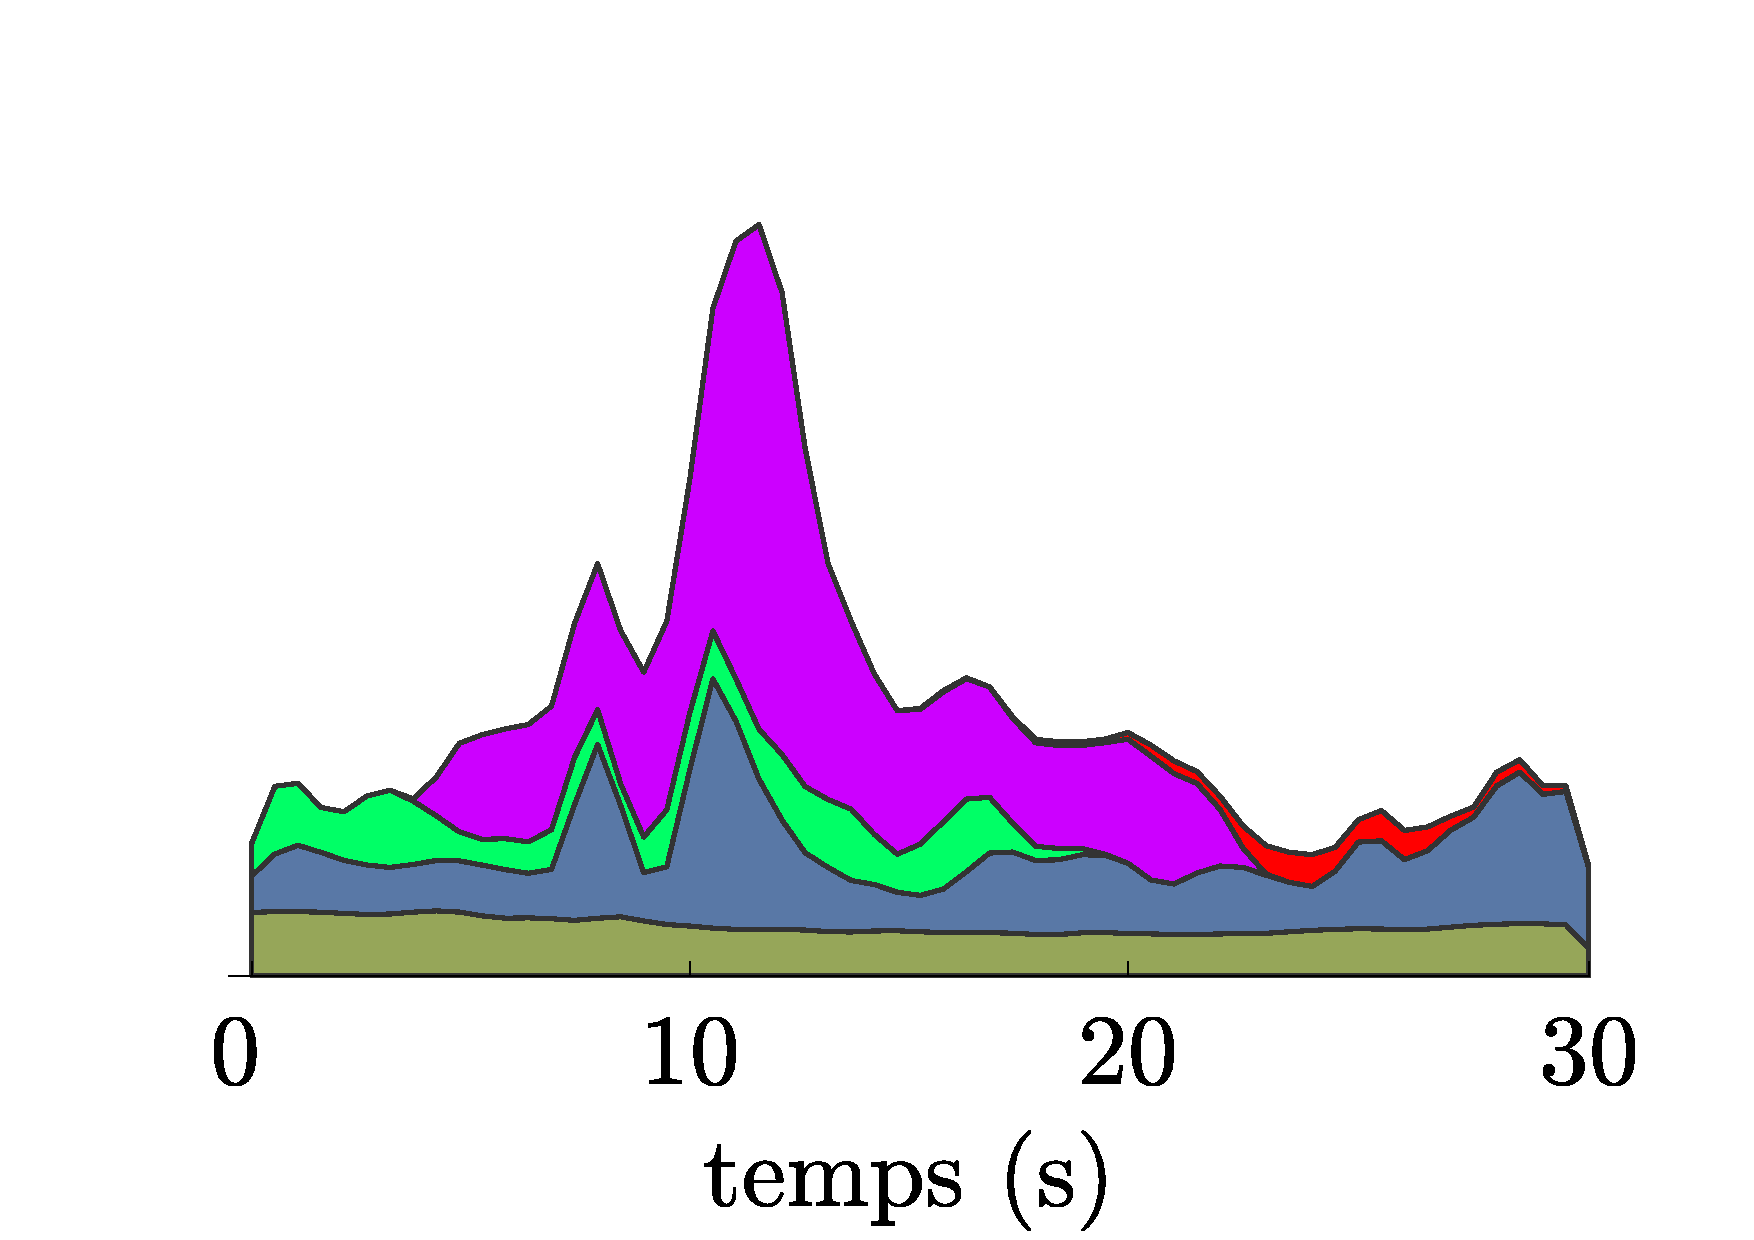
\includegraphics[width=5cm]{./figures/SimScene/exemple-timeDomain.pdf}\hfill
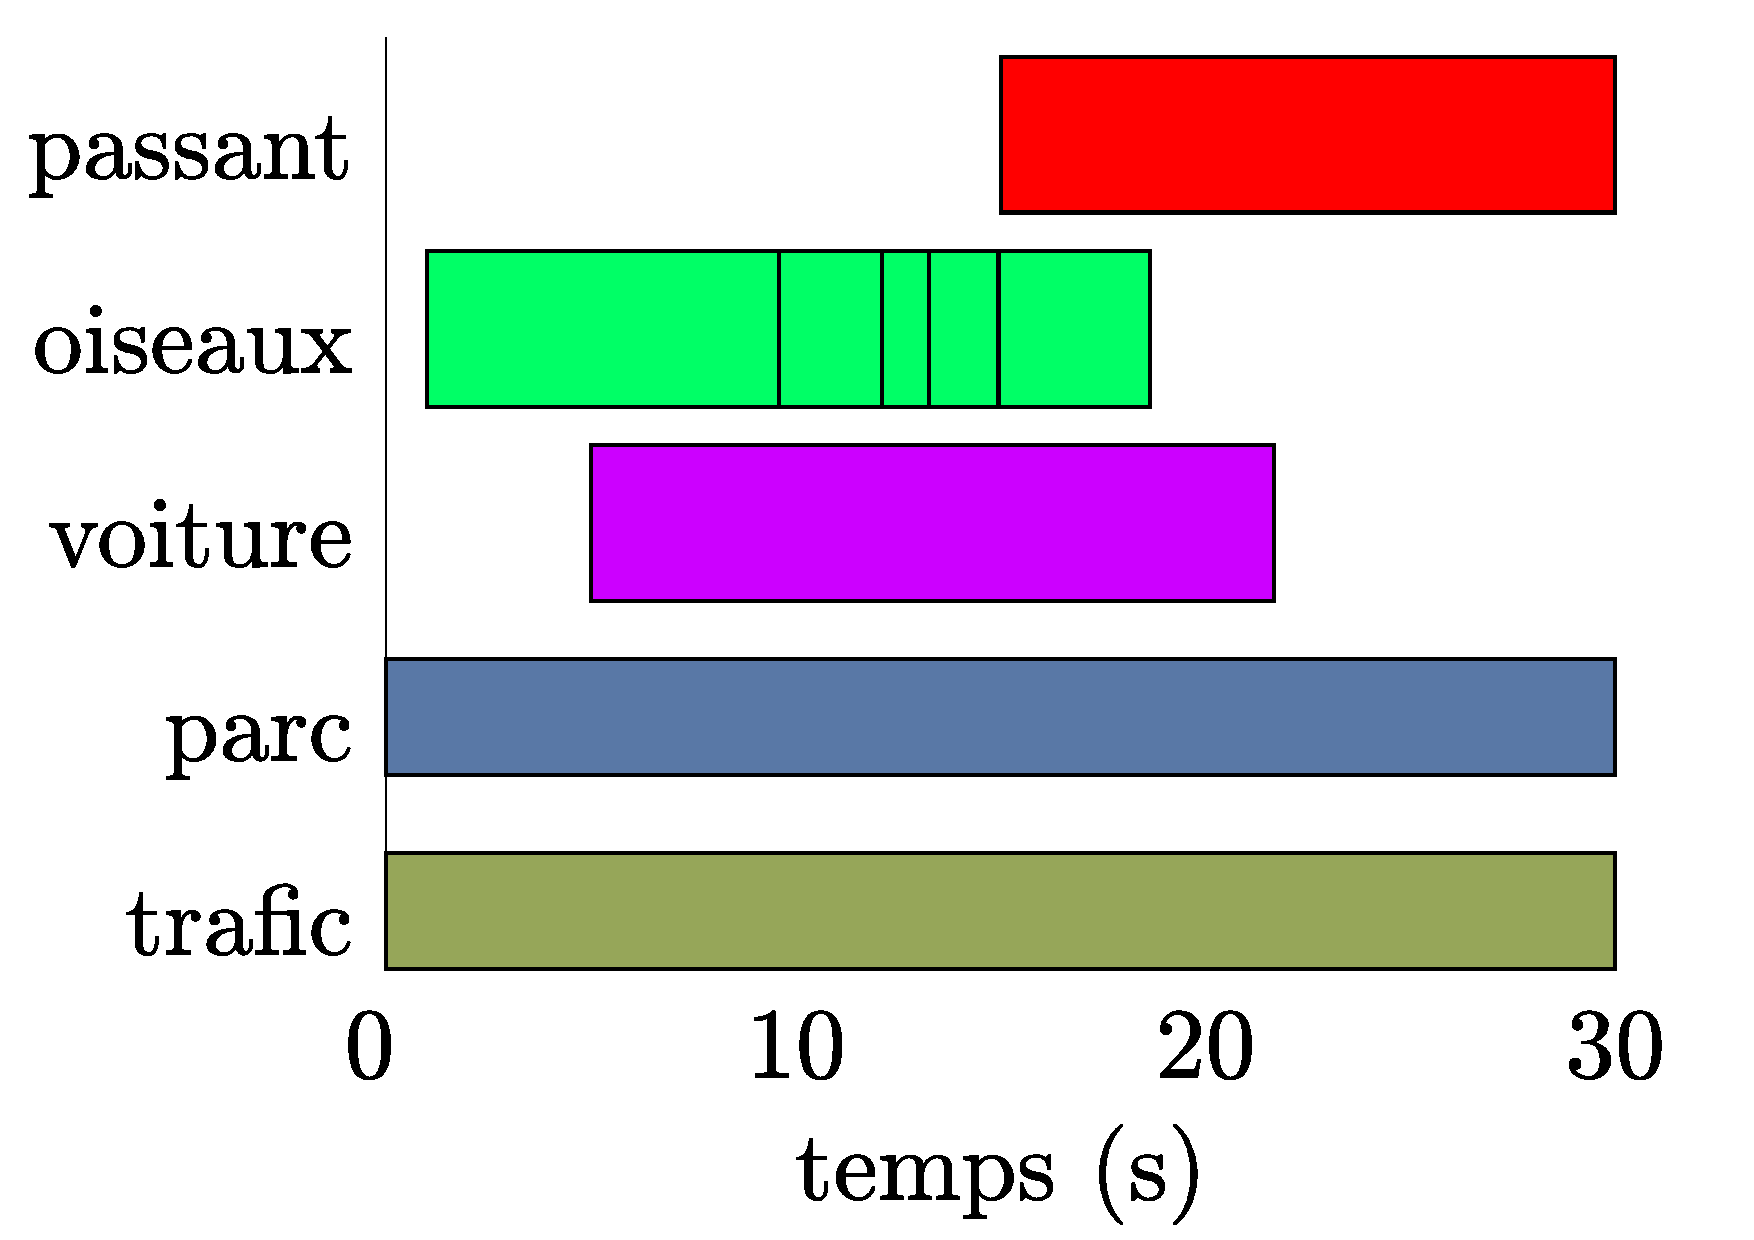
\includegraphics[width=5cm]{./figures/SimScene/exemple-pianoRoll.pdf}\hfill
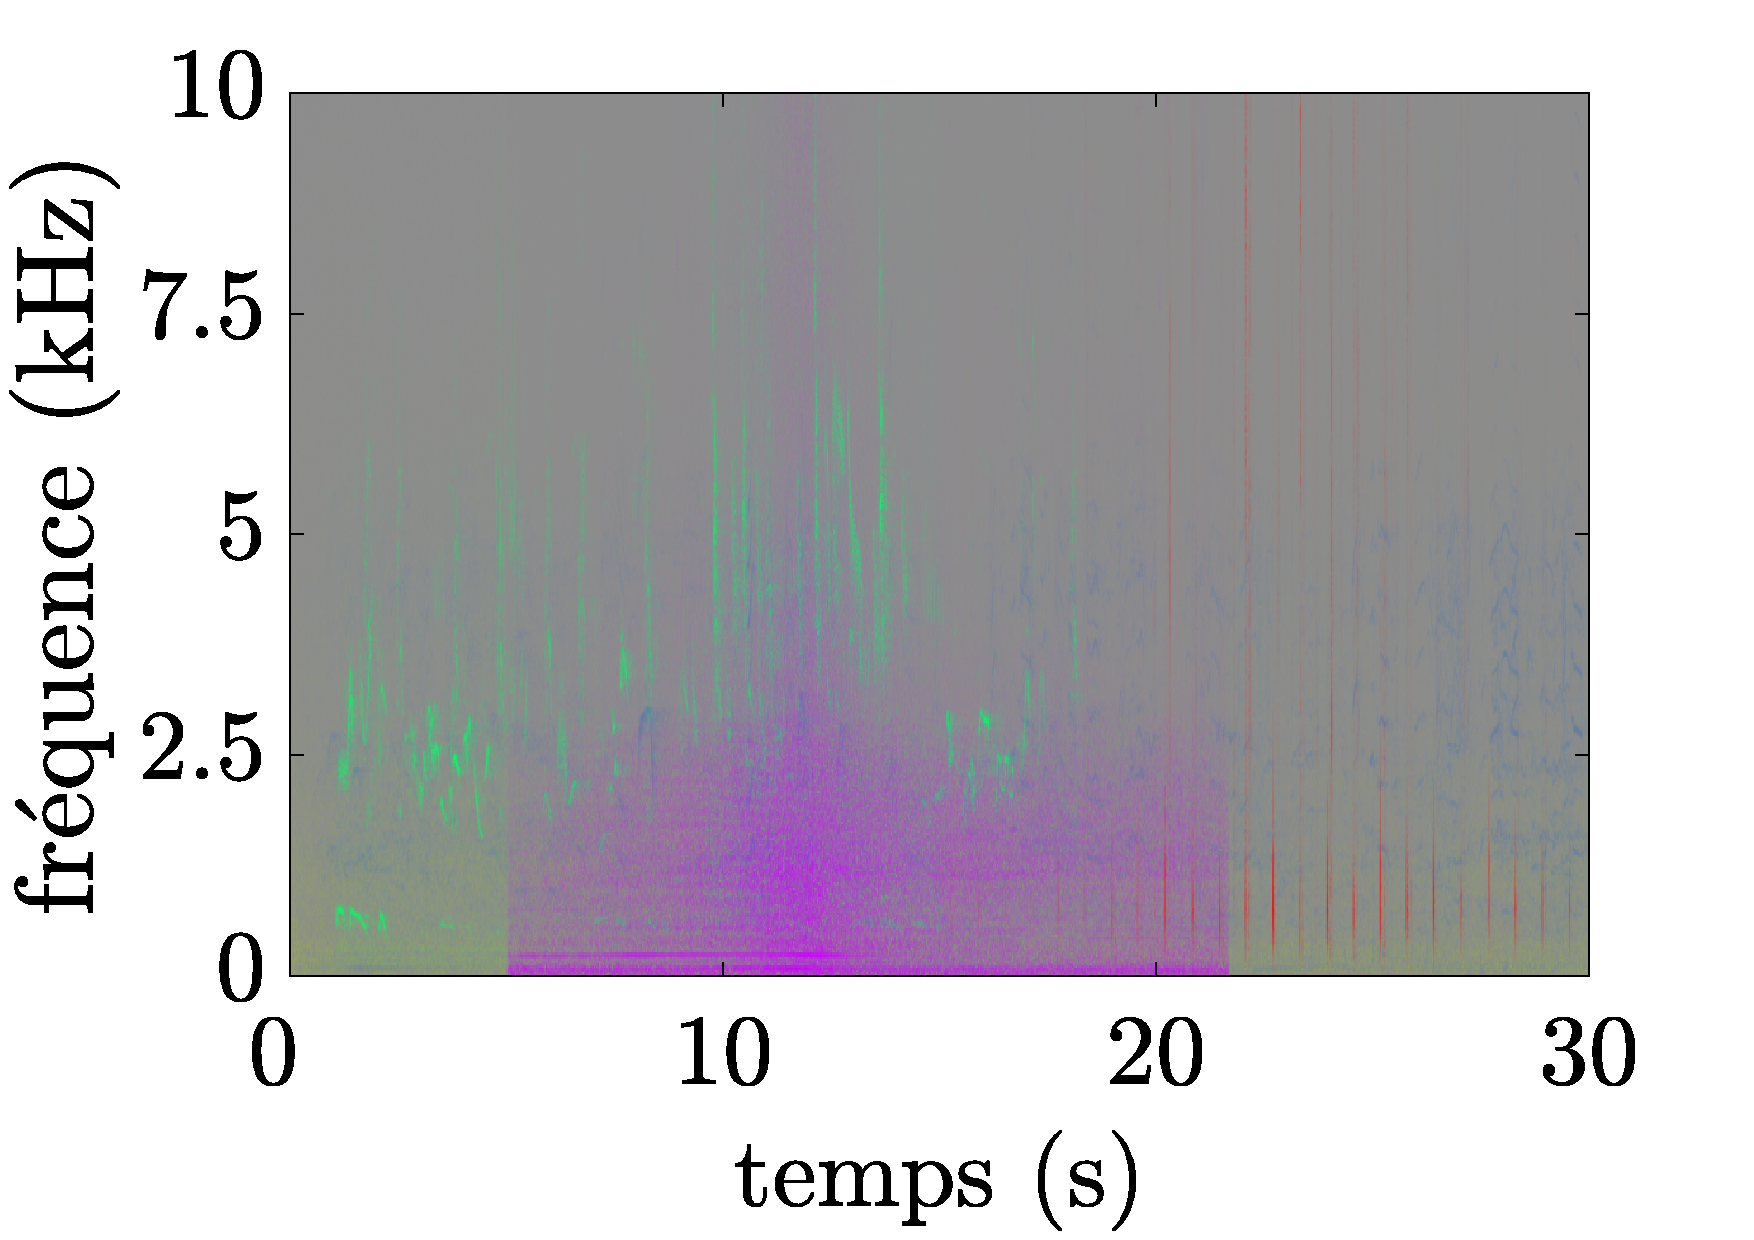
\includegraphics[width=5cm]{./figures/SimScene/exemple-spectrum.pdf}
\caption{Représentation temporelle (à gauche), \textit{Piano Roll} (au centre) et spectrogramme (à droite) générés par \textit{SimScene} d'une scène composée, d'un bruit de fond \textit{trafic}(en vert foncé) et \textit{parc} (en gris) et d'évènements \textit{oiseaux} (en vert), \textit{voiture} (en magenta) et \textit{passant} (en rouge).}\label{fig:somefiglabel}
\end{figure}

La génération de scènes avec \textit{SimScene} peut se faire selon 2 modes. Dans le mode \textit{abstract}, l'utilisateur renseigne lui-même les échantillons sonores présents dans la scène et chaque paramètre permettant de créer des scènes complètement artificiels. \`A l'inverse, dans le mode \textit{replicate}, le schéma de la scène s'appuie sur un fichier texte où la position d'évènements sonore (début et fin) et leur classe de son correspondante sont détaillées. Ce mode permet de reproduire des scènes avec la même organisation temporelle que celle des scènes réelles qui ont servies de référence.\\

L'outil a déjà été utilisé pour des études relatifs au payage sonore \cite{lafay2015approaching} où l'outil permet facilement la création de scènes sonores et ainsi d'estimer les classes de sons présentes et leur niveau sonore. \'Egalement, le simulateur a permis la réalisation de corpus de jeu de donnée pour le DCASE challenge \cite{stowell2015detection} dans le cas de la tâche de détection d'évènement sonores \cite{lagrange2015evaluation}. 

\textit{SimScene} nécessite d'avoir une base de données de sons isolés, appelée corpus élémentaire, devant être suffisamment représentatif. De plus, la qualité de chaque audio (rapport Signal/Bruit, échantillonnage) doit être suffisante pour que leurs juxtapositions ne viennent pas détériorer le rendu final.


\section{Création d'un corpus élémentaire d'échantillons audio}

\subsection{Recherche en ligne des échantillons audio}

La base de données de sons utilisée dans cette étude comprend un ensemble de classes de sons isolés (oiseaux, voiture, klaxon  \dots) qui contiennent chacune plusieurs échantillons (\textit{oiseaux01.wav}, \textit{oiseaux02.wav} \dots) pour permettre une grande variabilité dans les mixtures sonores créées. La plupart des échantillons sont trouvés sur des sites en ligne de sons \footnote{\url{www.freesound.org}} \footnote{\url{www.universalsoundbank.com}} et à l'aide de la base de données constituée dans  \cite{salamon_dataset_nodate}. Leur base de données comprend en tout plus de 8000 fichiers audio, collectés également sur le site \textit{freesound.org}, d'une durée inférieure à 4 secondes, répartis en 10 classes de sons : ventilation, klaxon de voiture, enfants qui joue, chien qui aboie, sonnerie, moteur en fonctionnement, coup de feu, marteau-piqueur, sirène et musique dans la rue. L'ensemble des échantillons a été trié afin de ne conserver que les audio ayant un rapport signal à bruit élevé et un échantillonnage de 44,1 kHz. \`A partir de la liste des noms des fichiers originaux fournis avec cette base de données, les fichiers audio sont récupérés dans leur intégralité sur le site internet et intégrés dans la base de données.\\
Afin d'obtenir un rapport signal à bruit acceptable, certains audio ont été filtrés à l'aide du logiciel d'Audacity. D'autres signaux ont, quant à eux, été tronqués ou bien divisés en plusieurs fichiers afin d'obtenir des durées convenables.

\subsection{Enregistrements de passages de véhicules}
S'il est possible de trouver l'ensemble des classes de son avec une qualité suffisante en ligne, dans le cas de la classe \textit{voiture}, étant la source sonore d'intérêt, il était nécessaire de réaliser des enregistrements de passages de véhicules contrôlés sur une piste d'essai afin de posséder un ensemble varié et maitrisé de vitesses et de modèles de véhicules. Pour cela, 2 véhicules à motorisation essence (Renault Mégane, Renault Sénic) et 2 autres à motorisation diesel (Renault Clio, Dacia Sandero) ont été enregistrées en suivant un plan de mesure défini comprenant plusieurs vitesses stabilisées à différents rapports de vitesses ainsi que des phases d'accélération et de freinage du véhicule.

\begin{table}[!htb]
    \begin{minipage}{.5\linewidth}
      \centering
        \begin{tabular}{|c|c|lllll}
\cline{2-7}
\multicolumn{1}{l|}{} & \multicolumn{1}{l|}{\textbf{Rapport}} & \multicolumn{1}{l|}{\textbf{1}} & \multicolumn{1}{l|}{\textbf{2}} & \multicolumn{1}{l|}{\textbf{3}} & \multicolumn{1}{l|}{\textbf{4}} & \multicolumn{1}{l|}{\textbf{5}} \\ \hline
\multicolumn{1}{|c|}{\multirow{8}{*}{\begin{tabular}[c]{@{}c@{}}\textbf{Vitesse}\\   \textbf{stabilisée}\\   \textbf{(km/h)}\end{tabular}}} & \textbf{20} & \multicolumn{1}{l|}{$\times$} & \multicolumn{1}{l|}{} & \multicolumn{1}{l|}{} & \multicolumn{1}{l|}{} & \multicolumn{1}{l|}{} \\ \cline{2-7} 
\multicolumn{1}{|c|}{} & \textbf{30} & \multicolumn{1}{l|}{} & \multicolumn{1}{l|}{$\times$} & \multicolumn{1}{l|}{$\times$} & \multicolumn{1}{l|}{} & \multicolumn{1}{l|}{} \\ \cline{2-7} 
\multicolumn{1}{|c|}{} & \textbf{40} & \multicolumn{1}{l|}{} & \multicolumn{1}{l|}{$\times$} & \multicolumn{1}{l|}{$\times$} & \multicolumn{1}{l|}{$\times$} & \multicolumn{1}{l|}{} \\ \cline{2-7} 
\multicolumn{1}{|c|}{} & \textbf{50} & \multicolumn{1}{l|}{} & \multicolumn{1}{l|}{} & \multicolumn{1}{l|}{$\times$} & \multicolumn{1}{l|}{$\times$} & \multicolumn{1}{l|}{} \\ \cline{2-7} 
\multicolumn{1}{|c|}{} & \textbf{60} & \multicolumn{1}{l|}{} & \multicolumn{1}{l|}{} & \multicolumn{1}{l|}{} & \multicolumn{1}{l|}{$\times$} & \multicolumn{1}{l|}{$\times$} \\ \cline{2-7} 
\multicolumn{1}{|c|}{} & \textbf{70} & \multicolumn{1}{l|}{} & \multicolumn{1}{l|}{} & \multicolumn{1}{l|}{} & \multicolumn{1}{l|}{$\times$} & \multicolumn{1}{l|}{$\times$} \\ \cline{2-7} 
\multicolumn{1}{|c|}{} & \textbf{80} & \multicolumn{1}{l|}{} & \multicolumn{1}{l|}{} & \multicolumn{1}{l|}{} & \multicolumn{1}{l|}{} & \multicolumn{1}{l|}{$\times$} \\ \cline{2-7} 
\multicolumn{1}{|c|}{} & \textbf{90} & \multicolumn{1}{l|}{} & \multicolumn{1}{l|}{} & \multicolumn{1}{l|}{} & \multicolumn{1}{l|}{} & \multicolumn{1}{l|}{$\times$} \\ \hline
\textbf{Total} & 14 &  &  &  &  &  \\ \cline{1-2}
\end{tabular}
    \end{minipage}
    \begin{minipage}{.5\linewidth}
      \centering
\begin{tabular}{|c|c||c|c|}
\hline
\multicolumn{2}{|c||}{\textbf{Freinage}} & \multicolumn{2}{c|}{\textbf{Accélération}} \\ \hline
\multicolumn{1}{|c|}{\begin{tabular}[c]{@{}c@{}}\textbf{Vitesse}\\  \textbf{(km/h)}\end{tabular}} & \multicolumn{1}{c||}{\textbf{Rapport}} & \multicolumn{1}{c|}{\begin{tabular}[c]{@{}c@{}}\textbf{Vitesse}\\  \textbf{(km/h)}\end{tabular}} & \multicolumn{1}{c|}{\textbf{Rapport}} \\ \hline
50 → 0 & 3 → 2 & 0 → 30 & 1 → 2 \\ \hline
40 → 0 & 2 → 2 & 0 → 40 & 1 → 2 \\ \hline
50 → 30 & 3 → 2 & 20 → 40 & 1 → 3 \\ \hline
60 → 40 & 4 → 3 & 30 → 50 & 2 → 3 \\ \hline
70 → 50 & 4 → 3 & 40 → 60 & 3 → 4 \\ \hline
80 → 50 & \begin{tabular}[c]{@{}l@{}}4 ou 5\\ → 3\end{tabular} & 50 → 70 & \begin{tabular}[c]{@{}l@{}}3 → \\ 4 ou 5\end{tabular} \\ \hline
\end{tabular}
    \end{minipage}%
    \caption{Ensemble de mesures réalisées sur pistes avec des passages de véhicules à vitesses stabilisée (à gauche) et en accélération et freinage (à droite)} 
\end{table}

Les enregistrements ont été réalisés sur la piste d'essais de l'Ifsttar de Nantes le 7 et 8 juillet 2016 à l'aide du système d'acquisition Sound Device 702, la position du microphone a respecté la norme de mesure de bruit au passage S 31-119 et fut donc situé à 7 m de la piste à une hauteur de 1m50. Enfin, les conditions météorologiques étaient satisfaisantes (temps clair et dégagé, température à l'ombre de 25$\degree$ C , vitesse moyenne du vent inférieure à 2 m/s). Les enregistrements sont ensuite extraits en fichiers audio en format .wav échantillonnés à 44,1 kHz.

Afin d'obtenir des échantillons de qualité suffisante, la présence d'oiseaux dans les enregistrements a été atténuée à l'aide d'un filtre médian \cite{fitzgerald_harmonic/percussive_2010} appliqué dans la bande de fréquence $\left[2500 - 6500\right]$ Hz, correspondante aux fréquences d'émission des oiseaux. Ce filtre consiste à définir une fenêtre et à attribuer la valeur médiane de cette fenêtre à l'élément central. Puisque les aspects à la fois temporels et fréquentiels sont à prendre en compte, la fenêtre du filtre est de forme rectangulaire de dimension $5 \times 9$ (96 Hz $\times$ 230 ms). Un exemple de l'application de cette fenêtre est présenté en Figure \ref{fig:filtre_median}\\

\begin{figure}[t]
\centering
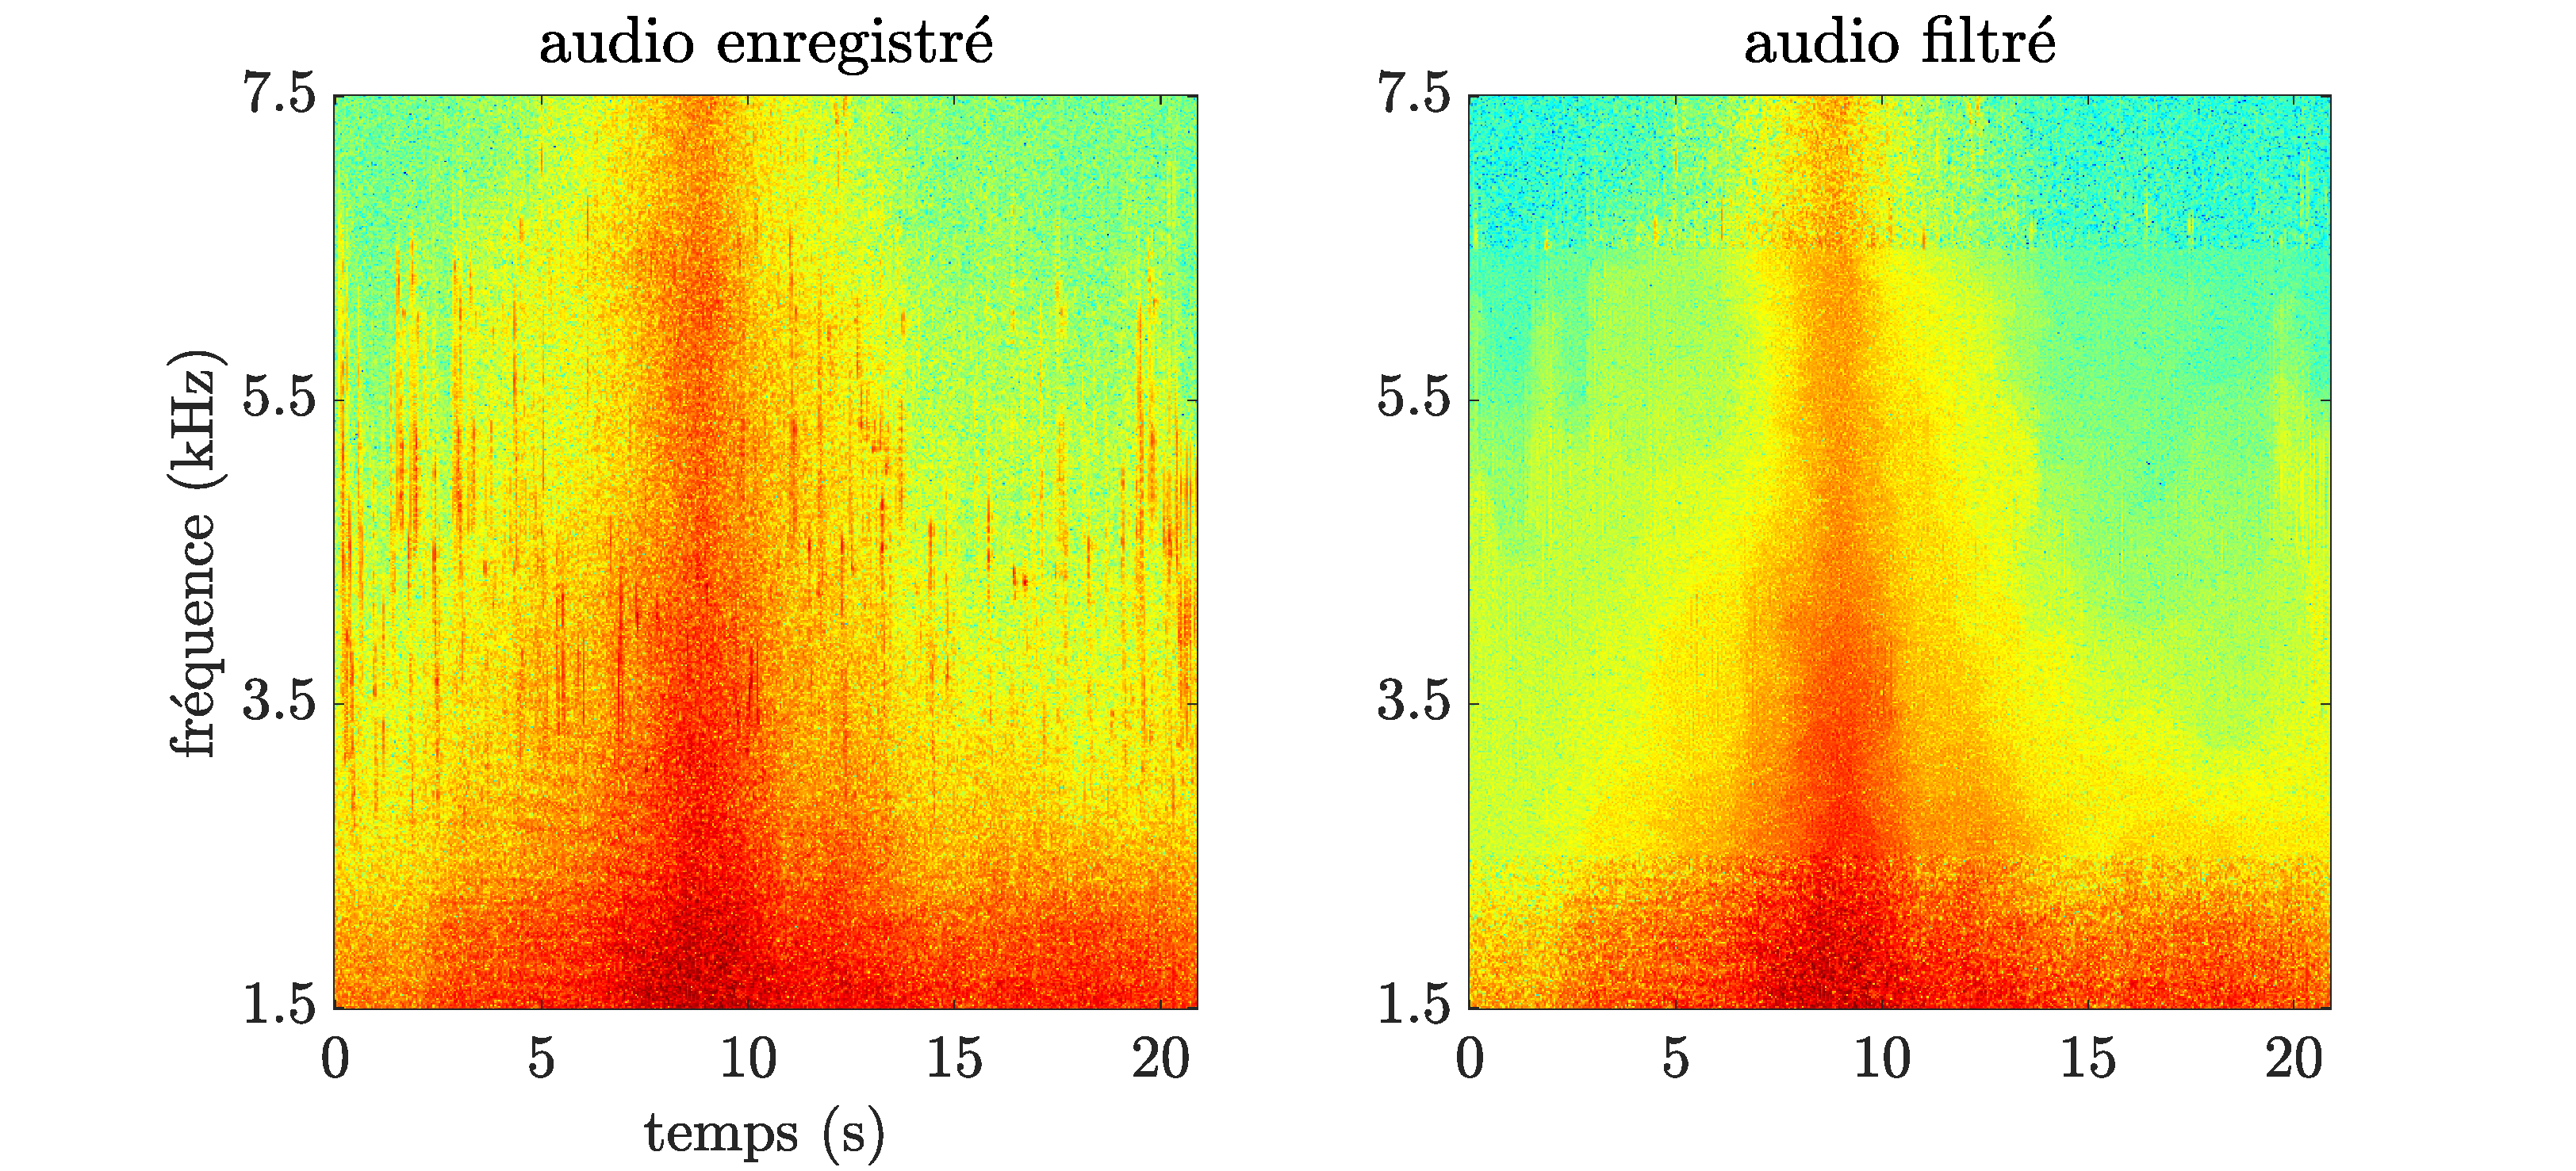
\includegraphics[width=.9\textwidth]{./figures/autres/filtrageMedian_VL1_R3_40_FR.pdf}
\caption{Zoom du spectrogramme (nombre de point $w = 2^{12}$ avec 50 $\%$ de recouvrement) dans la bande de fréquence $\left[1500-7500 \right]$ Hz d'un enregistrement de passage de véhicule (véhicule Renault, rapport 3, 40 km/h). \`A gauche, l'enregistrement original, à droite l'enregistrement filtré par le filtre médian.}
\label{fig:filtre_median}
\end{figure}


Même si elle reste persistante sur certains enregistrements, la présence des oiseaux est fortement atténuée sans toutefois dégrader la qualité perceptive du signal global du véhicule.\\

\subsection{Composition du corpus élémentaire complet}

La base de données est alors divisée en deux catégories. Une première comprend les évènements sonores courts allant de 1 seconde (klaxon, aboiement de chien) à plusieurs dizaines de secondes (passages de voitures, sirènes d'ambulances). Ces éléments permettent de générer les évènements sonores émergeant dans une scène. Une seconde catégorie est composée des sons de durées plus longues (1 min à 2 min) qui vont permettre de construire le bruit de fond utile à la création de l'ambiance sonore générale de la scène (chants d'oiseaux continu, voix d'enfants dans une cours de récréation, trafic routier continu \dots).

Les enregistrements des passages de voitures sont, quant à eux, séparés en deux parties : les enregistrements issus des deux  véhicules Renault Mégane et Renault Clio sont inclus dans le corpus élémentaire afin de construire les scènes sonores, les autres échantillons des deux autres voitures (Renault Scénic, Dacia Sandero) serviront dans les chapitres \ref{chap:ambiance} et \ref{chap:grafic} afin de construire le dictionnaire de la NMF et ainsi éviter toute problématique de surapprentissage.
Les échantillons sont ensuite séparés en deux classes de sons : \textit{voiture Ville} (si la vitesse stabilisée ou finale est inférieure ou égale à 50 km/h) et \textit{Voiture Route} (si la vitesse stabilisée ou finale est supérieure à 50 km/h). L'ensemble des fichiers audio est en format .wav échantillonnés à 44,1 kHz. La base de données finale est résumée dans le Tableau \ref{tab:dataBaseEv} pour les évènements sonores et dans le Tableau \ref{tab:dataBaseBcg} pour les bruits de fond sonores.

\begin{table}[h]
\centering
\begin{tabular}{m{5cm} c |m{5cm} c}
\hline
\toprule
\textbf{Classe de son} & \textbf{Nombre} & \textbf{Classe de son} & \textbf{Nombre} \\
\midrule
Aboiement de chien & 34 & Porte de voiture & 5\\ 
\rowcolor[HTML]{C0C0C0}
Balais & 6 & Roulement de valise & 5 \\ 
Bruit de chantier (marteau, perceuse \dots) & 12 & Sirène & 9 \\ 
\rowcolor[HTML]{C0C0C0}
Bruit de rue & 24 & Sonnette & 5 \\ 
Camion & 4 & Toussotement & 7\\ 
\rowcolor[HTML]{C0C0C0}
Cloches d'églises & 8 & Train & 7 \\ 
Klaxon & 24 & Tram & 7 \\
\rowcolor[HTML]{C0C0C0}
Oiseaux & 30 & Voiture à l'arrêt & 7 \\ 
Orage & 3 & Voiture ville & 28 \\ 
\rowcolor[HTML]{C0C0C0}
Pas dans la ville & 11 & Voiture route & 16 \\ 
Pas dans un parc & 16 & Voix (rire, 1 ou 2 mots) & 24 \\
\rowcolor[HTML]{C0C0C0}
Porte de maison & 5 &  \textbf{Total} & \textbf{321}\\ 
\bottomrule
\end{tabular}
\caption{Composition de la base de données pour les évènements sonores}
\label{tab:dataBaseEv}
\end{table}

\begin{table}[h]
\centering
\begin{tabular}{m{5cm} c |m{5cm} c}
\toprule
\textbf{Classe de son} & \textbf{Nombre} & \textbf{Classe de son} & \textbf{Nombre} \\ \midrule
Brouhaha de foule & 15 & Pluie & 14 \\ 
\rowcolor[HTML]{C0C0C0}
Brouhaha parc & 25 & Trafic routier & 9 \\
Chantier & 28 & Vent dans les arbres & 15 \\ 
\rowcolor[HTML]{C0C0C0}
Cours de récréation & 12 & Ventilation & 10 \\ 
Oiseaux & 25 & \textbf{Total} & \textbf{153} \\ 
\bottomrule
\end{tabular}
\caption{Composition de la base de données pour les bruits de fond}
\label{tab:dataBaseBcg}
\end{table}


La classe de son \textit{bruit rue} résume les nombreux bruits, le plus souvent très bref, dont la source sonore n'a pas pu être déterminée. De la même façon, les sons relatifs à un chantier en construction (marteau-piqueur, marteau, perceuse) sont regroupés en une seule classe par soucis de simplification.

À partir de ce corpus constitué, disponible en ligne\footnote{\url{https://zenodo.org/record/1213793}}, il est possible de réaliser des corpus de scènes sonores urbaines. En vue d'évaluer les performances lors d'une utilisation proche de mesures faites en ville, deux corpus de scènes sonores urbaines sont construits.

\section{Corpus d'évaluation \textit{Ambiance}}
\label{part:corpus_ambiance}
Dans un premier temps le choix est fait de générer un corpus où la présence de chaque source est définie selon sa classe de son et où les niveaux sonores du trafic sont calibrés. Ce corpus a vocation à étudier le comportement de la NMF selon certaines sources sonores isolées et selon la prédominance du trafic routier dans les scènes.

\begin{figure}[ht]
\centering
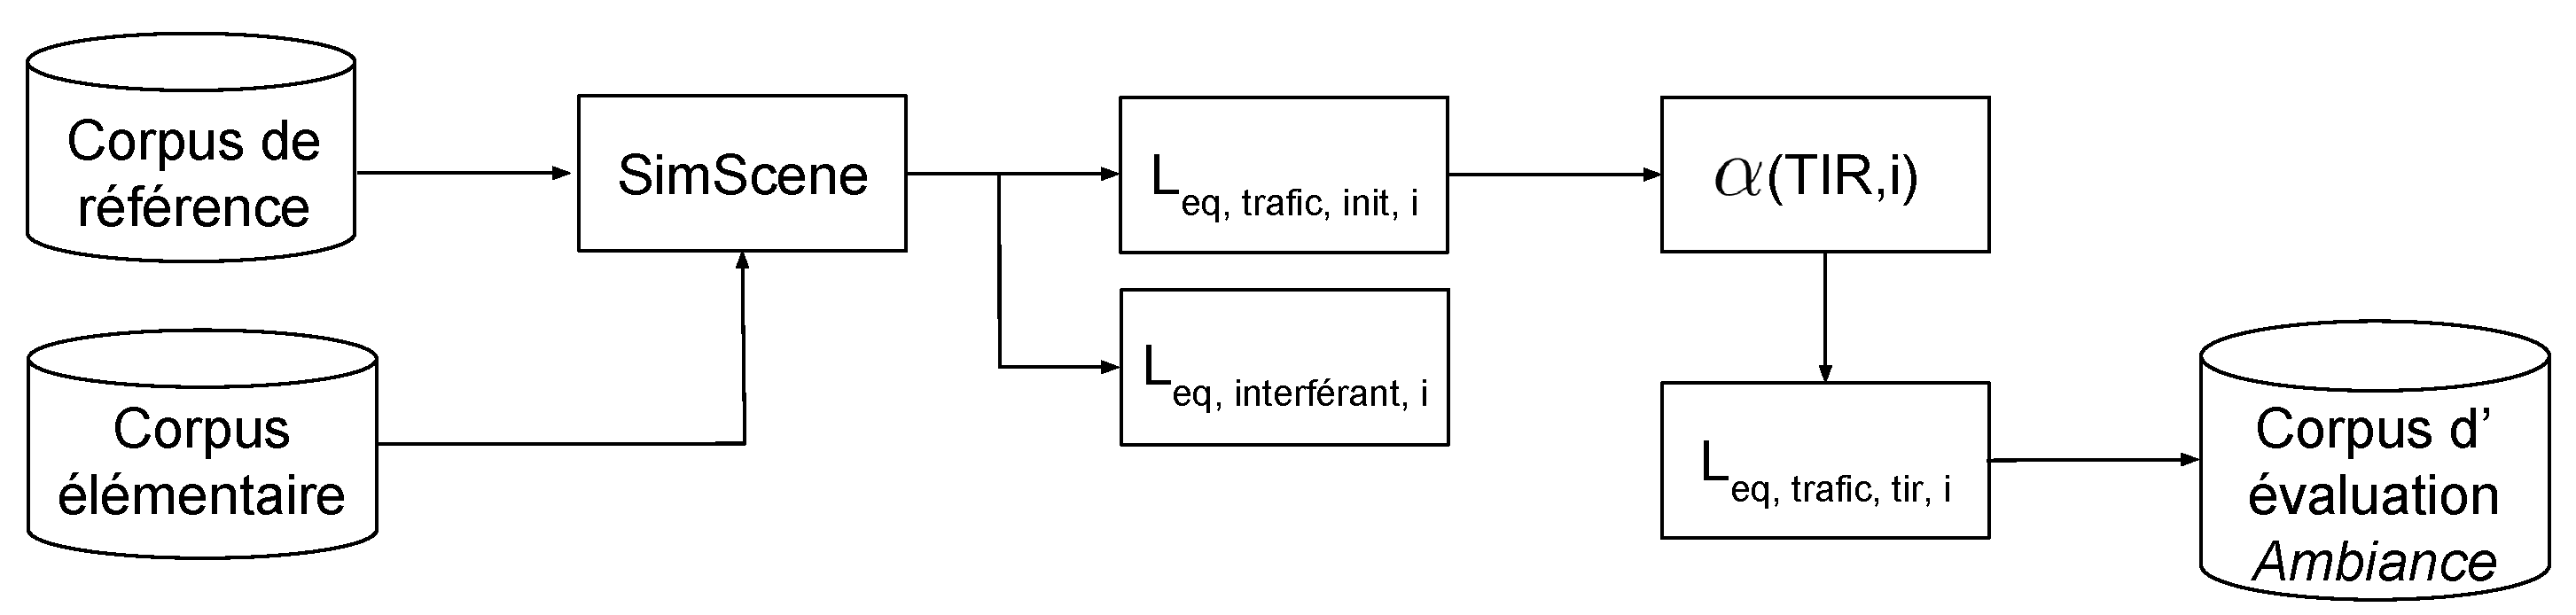
\includegraphics[width=.9\linewidth]{./figures/autres/TIR_ambiance.pdf}
\caption{Diagramme bloc de la pondération du signal trafic selon la scène $i$ et le TIR}
\label{fig:bloc_diagram_tir}
\end{figure}


Nommé \textit{Ambiance}, ce premier corpus consiste en un ensemble de 6 sous-corpus de 25 scènes ayant chacune une durée de 30 secondes. Chaque sous-corpus mélange une composante \textit{trafic} avec une classe de son spécifique (appelée classe \textit{interférante}).
Ces 6 classes de sons sont résumées dans le Tableau \ref{tab:class_inter} avec les classes de sons inclues dans ces classes interférantes.

\begin{table}[]
\centering
\caption{Résumé des classes de sons inclues dans les classes interférantes, seules les classes \textit{alerte} et \textit{transport} ne contiennent pas de bruit de fond}
\label{tab:class_inter}
\begin{tabular}{lll}
\toprule
\textbf{Classe interférante}  & \multicolumn{1}{c}{\textbf{\'Evènement}}                                                & \multicolumn{1}{c}{\textbf{Bruit de fond}}  \\
          \toprule
alerte    & \begin{tabular}[c]{@{}l@{}}- Klaxon\\ - Sirène\end{tabular}                  & \multicolumn{1}{c}{-}                                                       \\ \hline
animaux   & \begin{tabular}[c]{@{}l@{}}- Oiseaux\\ - Aboiement de chien\end{tabular}                  & - Oiseaux                                                                   \\ \hline
climat    & - Orage                                                                      & \begin{tabular}[c]{@{}l@{}}- Vent dans les arbres\\ - Pluie\end{tabular}                    \\ \hline
humain    & - Voix                                                                       & - Brouhaha de foule                                                                     \\ \hline
transport & \begin{tabular}[c]{@{}l@{}}- Train\\ - Tramway\\ - Avion\end{tabular}        & \multicolumn{1}{c}{-}                                                       \\ \hline
mécanique & \begin{tabular}[c]{@{}l@{}}- Bruit de rue\\ - Bruit de chantier\end{tabular} & \begin{tabular}[c]{@{}l@{}}- Ventilation\\ - Bruit de chantier\end{tabular}\\
\bottomrule
\end{tabular}
\end{table}


Chaque scène comprend un background trafic ainsi que jusqu'à 5 passage de véhicule.
Pour les classes interférantes, leur présence dans chaque scène est systématique. Elle est définie selon un tirage d'une loi uniforme : une valeur aléatoire est tirée, selon sa valeur elle définit la présence ou non de la classe de son. Pour les évènements sonores, il y a autant de chance d'avoir une classe de son parmi celles inclues dans la classe interférante que d'avoir l'ensemble des classes de sons. Par exemple, dans le cas de la classe interférante \textit{animaux}, qui comprend 2 classes de sons, il y a 33 $\%$ de chance d'avoir la classe \textit{oiseaux}, 33 $\%$ de chance d'avoir des aboiements et 33 $\%$ de chance d'avoir les deux classes présentes. Pour le cas des signaux \textit{alerte}, comme la durée d'un klaxon est plus brève que celle d'une sirène, la répartition de la distribution est est modifié afin de mieux équilibrer la présence temporelle (10 $\%$ de chance d'avoir une sirène, 80 $\%$ de chance d'avoir un coup de klaxon et 10 $\%$ d'avoir les deux dans la même scène).
Dans le cas de \textit{climat} et \textit{mécanique}, d'autre bruits de fond peuvent également être présent là aussi équitablement répartit. Enfin pour la classe \textit{humain}, la présence d'une foule en bruit de fond est présente une fois sur deux.


Chaque scène générée possède alors un niveau sonore trafic initial $L_{eq,trafic,init}$ et un niveau sonore \textit{interférant}, $L_{eq,interferant}$. Elles sont, chacune, dupliquées ensuite 5 fois où le niveau sonore du trafic y est calibré tel que, pour une scène $i$, $L_{eq,trafic, tir, i} - L_{eq,interferant, i} = TIR$ avec $TIR = \lbrace$ -12 -6 0 6 12 $\rbrace$. Pour cela, les fichiers audio relatifs au trafic sont pondérés par un coefficient $\alpha$ afin d'obtenir le niveau sonore souhaité selon le $TIR$ avec

\begin{equation}
\alpha(TIR,i) = 10^{\sfrac{(TIR-TIR_{init,i})}{20}}
\end{equation}

où $TIR_{init,i} = L_{eq,trafic,init,i}-L_{eq,interferant,i}$. Les étapes sont résumés sous la forme d'un diagramme en bloc dans la Figure \ref{fig:bloc_diagram_tir}. Lorsque $TIR < 0$ dB, le signal trafic est plus faible que le signal interférant, à l'inverse lorsque $TIR>0$, le trafic devient la classe sonore prépondérante. 



En tout 750 scènes sont ainsi disponibles (6 sous-corpus $\times$ 25 scènes $\times$ 5 TIR) pour une durée totale du corpus de 6h15. Les scènes de ce corpus ne peuvent pas être assimilable à des enregistrements sonores réalisés en ville, mais permettront tout de même d'étudier le comportement des algorithmes d'estimation. 

\section{Corpus d'évaluation de scènes sonores urbaines réalistes}
\label{part:corpus_grafic}

Un second corpus est généré, basé sur des enregistrements sonores réalisés en ville. Ce corpus d'évaluation de Scènes sOnores Urbaines Réalistes (corpus SOUR) a pour vocation de tester les performances de la NMF sur des scènes similaires à des enregistrements sonore faits en ville. Pour cela, un corpus de référence constitué d'enregistrements audio est obtenu pour ensuite être écouté et annoté. Ces annotations permettent alors de reproduire ces enregistrements en scènes simulées (dit \textit{répliquées}) qui forment alors le corpus d'évaluation SOUR. L'ensemble des étapes est résumé sous forme de bloc dans la Figure \ref{fig:bloc_diagram_annotation}.

\begin{figure}[ht]
\centering
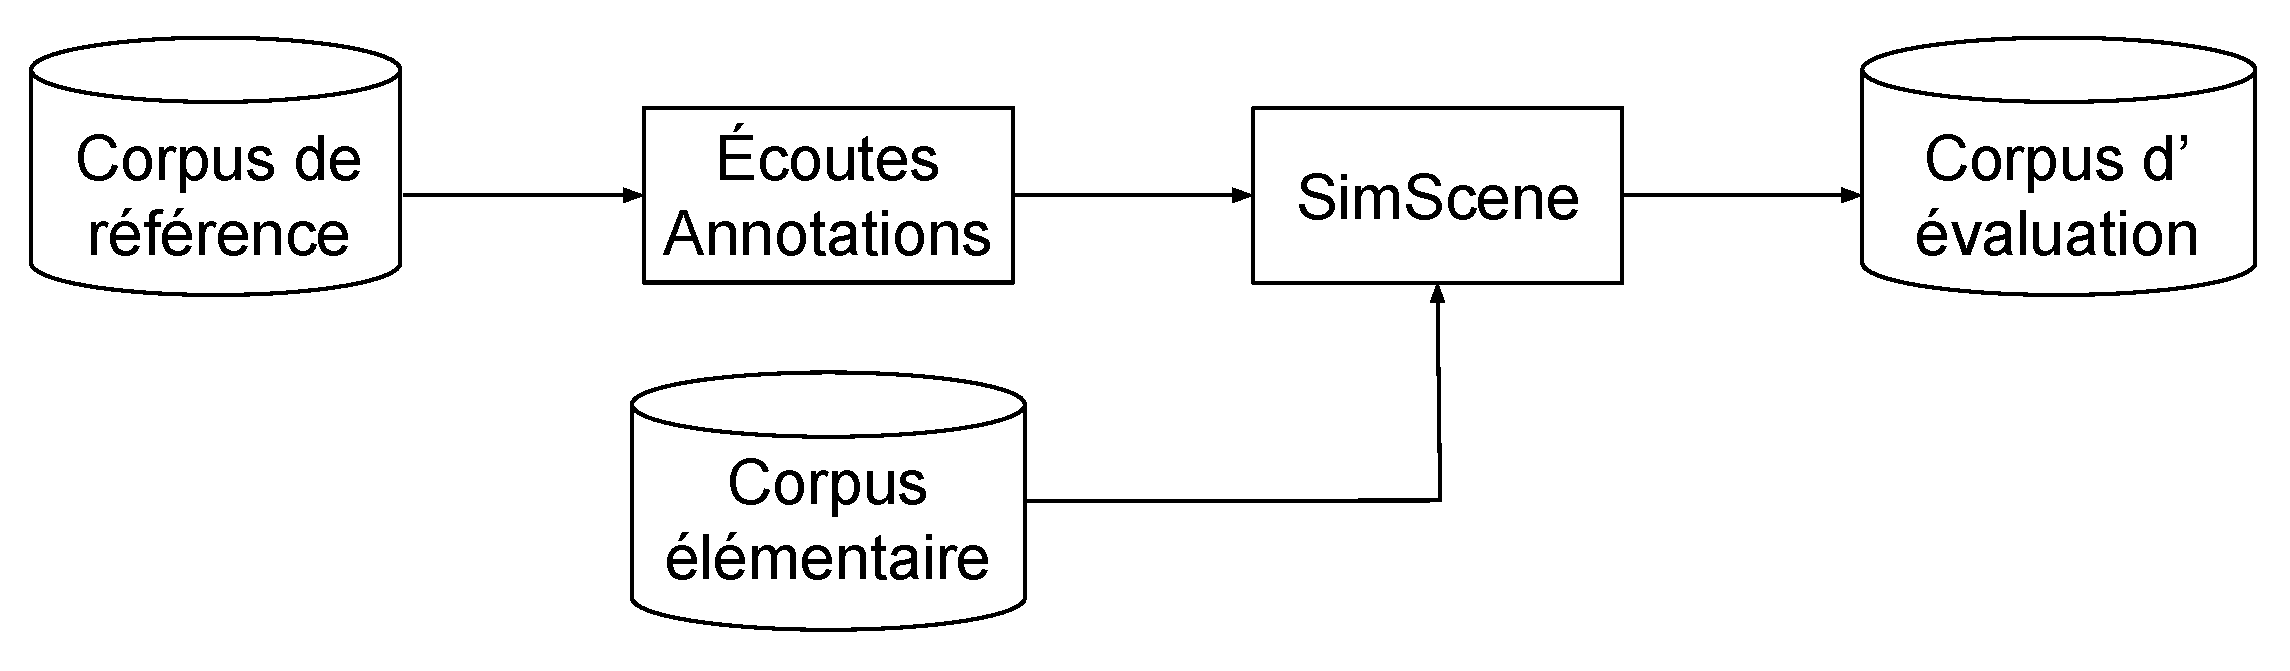
\includegraphics[width=.7\textwidth]{./figures/autres/bloc_diagram_annotation.pdf}
\caption{Diagramme bloc résumant la création du corpus d'évaluation de scènes sonores urbaines réalistes}
\label{fig:bloc_diagram_annotation}
\end{figure}

\subsection{Présentation des enregistrements audio de références}

Les enregistrements audio de références sont issus du projet GRAFIC \cite{aumond2017modeling} et ont été recueillis à pied dans le 13\ieme~arrondissement de la ville de Paris sur un parcours comprenant 19 points d'arrêts (Figure \ref{fig:parcoursGRAFIC}). Le parcours définit présente l'avantage de couvrir plusieurs ambiances sonores représentatifs d'un environnement sonore urbain (Tableau \ref{tab:resume19pts}).\\

\begin{figure}[hbtp]
\centering
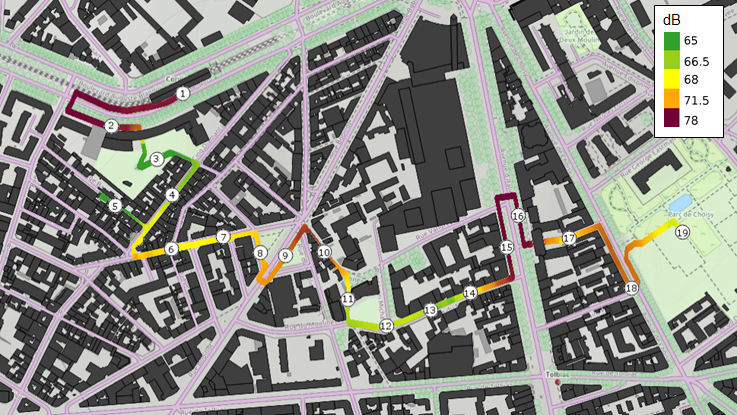
\includegraphics[width=.7\textwidth]{./figures/grafic/trajet_19pts.png}
\caption{Parcours réalisé par l'étude avec les 19 points de mesures avec le niveau sonore mesuré équivalent}
\label{fig:parcoursGRAFIC}
\end{figure}

Ce trajet a été parcouru sur deux jours (le 23/05/2015, jour 1, et le 30/05/2015, jour 2), deux fois par jour (le matin puis l'après-midi) dans un sens (d'est en ouest, EW) et dans l'autre (d'ouest en est, WE). L'enregistrement est réalisé par un système d'acquisition équipé d'un microphone ASASense omnidirectionnel situé sur un sac à dos porté par l'opérateur \cite{aumond2017modelling}. En tout, 76 enregistrements audio (19 points $\times$ 4 trajets) de 1 à 4 minutes sont disponibles. \\

\begin{table}[h]
\centering

\begin{tabular}{|c|p{6cm}||c|p{6cm}|}
\hline
\textbf{Point} & \textbf{Description  }                 & \textbf{Point} & \textbf{Description                                      } \\ \hline
1     & Large rue à deux voies        & 10    & Rue sans trafic près d’une école                  \\ \hline
2     & Large rue à deux voies        & 11    & Rue silencieuse sans trafic                       \\ \hline
3     & Parc calme                    & 12    & Rue avec un faible débit de trafic                \\ \hline
4     & Rue animé avec restaurant/bar & 13    & Rue avec un faible débit de trafic                \\ \hline
5     & Rue très calme                & 14    & Rue avec un faible débit de trafic                \\ \hline
6     & Rue animé avec restaurant/bar & 15    & Rue avec un fort débit de trafic                  \\ \hline
7     & Rue animé avec restaurant/bar & 16    & Rue avec un fort débit de trafic                  \\ \hline
8     & Parc situé le long d’une rue  & 17    & Rue piétonne calme situé entre deux rues bruyante \\ \hline
9     & Rue avec un trafic modéré     & 18    & Grand carrefour avec un trafic constant           \\ \hline
      &                               & 19    & Grand parc                                        \\ \hline
\end{tabular}
\caption{résumé des 19 points de mesures avec l'ambiance générale}
\label{tab:resume19pts}
\end{table}


\subsection{Écoutes des scènes sonores}

La première étape réalise un classement, selon quatre ambiances sonores (\textit{parc}, \textit{rue calme}, \textit{rue animée}, \textit{rue très animée} \cite{can_describing_2015}), des enregistrements sonores à partir des indications fournies dans \cite{aumond2017modeling} (résumé dans le Tableau \ref{tab:resume19pts}) et des écoutes faites (Tableau \ref{tab:classificationScene}).\\

\begin{table}[t]
\caption{Classification des scènes par ambiances sonores.}
\centering
\begin{tabular}{|c|c|*{19}{l|}}
\hline
\multicolumn{1}{|l|}{\textbf{Jour}} & \textbf{trajet}   & 1                        & 2                        & 3                        & 4                        & 5                        & 6                        & 7                        & 8                        & 9                        & 10                       & 11                       & 12                       & 13                       & 14                       & 15                       & 16                       & 17                       & 18                       & 19                       \\ \hline
\textbf{1} & \textbf{EW} & \cellcolor[HTML]{F56B00} & \cellcolor[HTML]{F56B00} & \cellcolor[HTML]{5AB25A} & \cellcolor[HTML]{FFCB2F} & \cellcolor[HTML]{FFCB2F} & \cellcolor[HTML]{F56B00} & \cellcolor[HTML]{FFCB2F} & \cellcolor[HTML]{5AB25A} & \cellcolor[HTML]{F56B00} & \cellcolor[HTML]{5AB25A} & \cellcolor[HTML]{FFCB2F} & \cellcolor[HTML]{F56B00} & \cellcolor[HTML]{FFCB2F} & \cellcolor[HTML]{FFCB2F} & \cellcolor[HTML]{F56B00} & \cellcolor[HTML]{9A0000} & \cellcolor[HTML]{FFCB2F} & \cellcolor[HTML]{F56B00} & \cellcolor[HTML]{5AB25A} \\ \hline
\textbf{1}  & \textbf{WE} & \cellcolor[HTML]{F56B00} & \cellcolor[HTML]{F56B00} &                          & \cellcolor[HTML]{FFCB2F} & \cellcolor[HTML]{FFCB2F} & \cellcolor[HTML]{FFCB2F} & \cellcolor[HTML]{FFCB2F} & \cellcolor[HTML]{FFCB2F} & \cellcolor[HTML]{F56B00} & \cellcolor[HTML]{F56B00} & \cellcolor[HTML]{FFCB2F} & \cellcolor[HTML]{F56B00} & \cellcolor[HTML]{FFCB2F} & \cellcolor[HTML]{FFCB2F} & \cellcolor[HTML]{9A0000} & \cellcolor[HTML]{9A0000} & \cellcolor[HTML]{FFCB2F} & \cellcolor[HTML]{F56B00} &  \\ \hline
\textbf{2} & \textbf{EW} & \cellcolor[HTML]{F56B00} & \cellcolor[HTML]{F56B00} & \cellcolor[HTML]{5AB25A} & \cellcolor[HTML]{FFCB2F} & \cellcolor[HTML]{FFCB2F} & \cellcolor[HTML]{FFCB2F} & \cellcolor[HTML]{FFCB2F} & \cellcolor[HTML]{FFCB2F} & \cellcolor[HTML]{F56B00} & \cellcolor[HTML]{F56B00} & \cellcolor[HTML]{FFCB2F} & \cellcolor[HTML]{F56B00} & \cellcolor[HTML]{FFCB2F} & \cellcolor[HTML]{F56B00} & \cellcolor[HTML]{9A0000} & \cellcolor[HTML]{9A0000} & \cellcolor[HTML]{FFCB2F} & \cellcolor[HTML]{F56B00} & \cellcolor[HTML]{5AB25A} \\ \hline
\textbf{2} & \textbf{WE} & \cellcolor[HTML]{F56B00} & \cellcolor[HTML]{F56B00} & \cellcolor[HTML]{5AB25A} & \cellcolor[HTML]{FFCB2F} & \cellcolor[HTML]{FFCB2F} & \cellcolor[HTML]{FFCB2F} & \cellcolor[HTML]{FFCB2F} & \cellcolor[HTML]{FFCB2F} & \cellcolor[HTML]{F56B00} & \cellcolor[HTML]{FFCB2F} & \cellcolor[HTML]{FFCB2F} & \cellcolor[HTML]{FFCB2F} & \cellcolor[HTML]{FFCB2F} & \cellcolor[HTML]{FFCB2F} & \cellcolor[HTML]{9A0000} & \cellcolor[HTML]{9A0000} & \cellcolor[HTML]{FFCB2F} & \cellcolor[HTML]{9A0000} & \cellcolor[HTML]{5AB25A} \\ \hline
\end{tabular}

\vspace{0.5cm}


\begin{tabular}{|p{1.5cm}|l|p{0.001cm}|p{2cm}|l|p{0.001cm}|p{2cm}|l|p{0.001cm}|p{2.75cm}|l|p{0.001cm}|p{2.45cm}|l|}

\hhline{|-|-|~|-|-|~|-|-|~|-|-|~|-|-|}
Parc & {\cellcolor[HTML]{5AB25A}} & & Rue calme & {\cellcolor[HTML]{FFCB2F}} & & Rue animée & {\cellcolor[HTML]{F56B00}} & &  Rue très animée & {\cellcolor[HTML]{9A0000}} & & Non renseigné & \\
\hhline{|-|-|~|-|-|~|-|-|~|-|-|~|-|-|}

\end{tabular}
\label{tab:classificationScene}
\end{table}

Une majorité de scènes appartiennent à l'ambiance sonore \textit{rue calme} (35 scènes), 23 scènes appartiennent à l'ambiance \textit{rue animée}, 8 scènes à l'ambiance \textit{parc} et 8 scènes à l'ambiance \textit{rue très animée}. Plus de la moitié des points de mesures possèdent la même ambiance sur les 4 trajets. À l'exception du point 10, tous les points de mesures possèdent deux ambiances sonores voisines. Ces variations proviennent des variations des activités dans la journée (matin ou l'après-midi). Enfin, les points 3 et 19 du parcours 1-WE ne sont pas exploitables : le point 3 est pollué par un camion balayeur et le point 19 n'a pas été correctement enregistré. Au final, c'est 74 fichiers audio qui sont disponibles et utilisés pour créer des scènes sonores. Ces 74 enregistrements forment le \textit{corpus de référence}.

\subsection{Annotation des enregistrements sonores}\label{part:scene_annotation}

L'annotation des 74 enregistrements est ensuite réalisée qui consiste à écouter chaque fichier audio et à estimer les sources sonores présentes ainsi que leur temps de présence. Pour chaque enregistrement, l'ensemble des annotations est résumé dans un fichier texte. Un exemple d'annotation est présenté dans le Tableau \ref{tab:exemple_annotation}.\\

\begin{table}[h]
\centering
\begin{tabular}{lll}
\toprule
\textbf{évènements}    & $\mathbf{t_{init}}$ \textbf{(s)} & $\mathbf{t_{fin}}$ \textbf{(s)} \\ \midrule
bruit rue     & 0,00            & 8,50           \\
\rowcolor[HTML]{C0C0C0}
voix          & 0,00            & 44,00          \\
camion        & 1,00            & 56,10          \\
\rowcolor[HTML]{C0C0C0}
voix          & 36,50           & 42,30          \\
voiture Ville & 52,00          & 63,00          \\
\rowcolor[HTML]{C0C0C0}
voix          & 59,00           & 66,50         \\ \bottomrule
\end{tabular}
\caption{Exemple d'un fichier d'annotation pour la scène 1-EW-07.}
\label{tab:exemple_annotation}
\end{table}

\begin{table}
\centering
\begin{tabular}{L{2cm} | C{2cm} | C{2cm} | L{3cm} | C{2cm} | C{2cm}}
\toprule
\centering \small \textbf{Environnent sonore} & \small \textbf{Niveau sonore (dB)} & \small \textbf{Bruit de fond } & \small \centering \textbf{Évènement} & \small \textbf{Nombre évènement/min} & \small \textbf{Rapport Évènement-Bruit de fond (dB)} \\ \midrule

Parc              & 69,0        &
\begin{tabular}[c]{@{}l@{}}voix \\ sifflements \\ d'oiseaux \end{tabular} &
\begin{tabular}[c]{@{}l@{}}voiture ville \\ voix\\ sifflements\\ \hfill d'oiseaux \\ bruit de rue\\ bruit de pas\end{tabular}                                         &
\begin{tabular}[c]{@{}l@{}}1,6\\ 0,5 \\ 0,5 \\ \\ 0,5\\ 0,3\end{tabular}               &    \begin{tabular}[c]{@{}l@{}} 3,0 ($\pm$ 6,0) \\ 6,5 ($\pm$ 5,0) \\ 0,0 ($\pm$ 9,5) \\	\\ 6,7 ($\pm$ 4,5) \\ 4,0 ($\pm$ 7,0)\end{tabular}     \\\hline

Rue calme      & 70,2        &
\begin{tabular}[c]{@{}l@{}}trafic routier\\ \begin{tabular}[c]{@{}l@{}}sifflements \\ \hfill d'oiseaux \end{tabular}\end{tabular}       &
\begin{tabular}[c]{@{}l@{}}voiture ville \\ voix\\ bruit de rue\\ bruit de pas\\ sifflements \\ \hfill d'oiseaux \\  porte de maison\\ porte de voiture \\chantier \end{tabular} &
\begin{tabular}[c]{@{}l@{}}1,7\\ 0,7\\ 0,7\\ 0,5\\ 0,2\\  \\  0,2\\ 0,2 \\  0,1\end{tabular} & \begin{tabular}[c]{@{}l@{}} 7,6 ($\pm$ 4,6) \\ 8,2 ($\pm$ 4,0) \\ 7,6 ($\pm$ 4,2) \\ 8,0 ($\pm$ 5,0) \\ 3,0 ($\pm$ 5,8) \\ \\ 9,0 ($\pm$ 3,3) \\ 7,7 ($\pm$ 4,2) \\ 3,7 ($\pm$ 5,1) \end{tabular}
\\ \hline

Rue animée      & 73,5        & trafic routier                                                      & \begin{tabular}[c]{@{}l@{}}voiture ville \\ voix\\ bruit de pas\\ bruit de rue \\ klaxon\\ sifflements \\ \hfill d'oiseaux \\ porte de voiture\\ sirène \\ sonnette\end{tabular}                   & \begin{tabular}[c]{@{}l@{}}9,4 \\ 0,6 \\ 0,5\\ 0,4 \\ 0,3\\ 0,2\\ \\ 0,2\\ 0,1 \\ 0,1\end{tabular}  & \begin{tabular}[c]{@{}l@{}} 3,3 ($\pm$ 2,5) \\ 1,3 ($\pm$ 2,6) \\ -3,6 ($\pm$ 6,4) \\ 5,2 ($\pm$ 4,6) \\ 3,5 ($\pm$ 3,9)\\ 1,6 ($\pm$ 5,0)  \\ \\ 4,4 ($\pm$ 5,4) \\ 2,0 ($\pm$ 6,2) \\ 1,7 ($\pm$ 3,5) \end{tabular}\\ \hline

Rue très animée & 76,0 & trafic routier                                                      &
\begin{tabular}[c]{@{}l@{}}voiture ville\\ voix \\ klaxon \\ porte de voiture\\ sirène\\ bruit de pas\\ bruit de rue\end{tabular}                          
& 
\begin{tabular}[c]{@{}l@{}}40,9\\ 0,3\\ 0,3\\ 0,3\\ 0,2\\ 0,2\\ 0,2\end{tabular}  & \begin{tabular}[c]{@{}l@{}}2,3 ($\pm$ 1,3) \\ 1,3 ($\pm$ 1,1) \\ 2,7 ($\pm$ 4,1) \\ 3,6 ($\pm$5,4) \\ -3,0 ($\pm$ 4,2) \\ -3,6 ($\pm$ 5,8) \\ 5,1 ($\pm$ 4,7) \end{tabular}\\ \bottomrule
\end{tabular}
\caption{Niveau sonore et description des classes de sons les plus récurrentes dans l'environnement urbain (nombre d'évènements sonore par minute > 0.1/min).}
\label{tab:obsScene}
\end{table}



De ces annotations, il est possible d'estimer, par ambiance sonore, un niveau sonore moyen, les classes de sons qui caractérisent leur bruit de fond, les classes de sons catégorisées en évènements sonores ainsi que leur densité (nombre d'évènement par minute). Ces informations sont alors utilisées pour pouvoir recréer ces scènes par le mode \textit{abstract} de \textit{SimScene} (Tableau \ref{tab:obsScene}).\\

Sur l'ensemble des scènes sonores, 11 classes de sons sont identifiées en tant qu'évènement sonore (trafic routier, voix, sifflements d'oiseaux, bruit de rue, bruit de pas, porte de maison, porte de voiture, chantier, klaxon, sonette, sirène) et 3 classes de sons sont présentes en tant que bruit de fond sonore (brouhaha de foule, sifflements d'oiseaux, trafic routier continu).
Les sources sonores les plus communes sont \textit{voiture}, \textit{voix} et \textit{bruit rue}. En outre, en plus des classes de sons résumées dans le Tableau \ref{tab:obsScene}, de nombreuses autres classes de sons (\textit{aboiement de chien},\textit{bruit de balais}, \textit{toussotement}, \textit{passage d'avion}, \textit{roulement de valise}) entendus interviennent plus sporadiquement (nombre d'évènement/min < 0,1) et sont susceptibles d'intervenir dans les quatre ambiances sonores.

La composition des environnements sonore diffère entre eux : dans \textit{parc} la voix et les oiseaux sont les bruits de fond sonores principaux permettant d'établir l'ambiance sonore adéquate, puis, plus la rue est animée plus la part de la classe \textit{trafic} et celle de l'activité humaine (\textit{voix, bruit de pas}) sont prédominantes. À l'inverse, les classes de sons \og naturel \fg{} (\textit{oiseaux)} disparaissent progressivement.

Notons que dans \textit{rue calme}, \textit{animée} et dans \textit{parc}, le décompte des voitures est assez aisé. Il l'est beaucoup moins dans \textit{rue très animée} où un flot de véhicules peut être présent, le comptage y est alors très délicat car les véhicules peuvent être considérés à la fois comme bruit de fond et évènements sonore.
Sans étude perceptive sur le débit de véhicule à partir duquel les passages de véhicules deviennent un flux, une moyenne de 1 véhicule par seconde est alors considérée comme raisonnable. Un contrôle à l'écoute permet de vérifier que le rendu est satisfaisant. Le rapport nombre d'évènement/min renseigné dans le Tableau \ref{tab:obsScene} est donc soumis à une forte incertitude mais reste cependant cohérent avec les indications du débit moyen fournis dans \cite{aumond2017modeling} ($\approx$ 2000 véhicules/heure). \\

\subsection{Reproduction des enregistrements audio}

Afin d'obtenir des scènes les plus réalistes possibles, le choix a été fait de reproduire les 74 enregistrements à l'aide de leur annotation et du mode \textit{replicate} de \textit{SimScene}. Ce choix permet ainsi de s'assurer que la disposition des évènements sonores dans les mixtures sonore est la plus proche possible d'une structure temporelle écologiquement valide. La difficulté réside surtout dans l'estimation du \textit{event background ratio} pour les évènements sonores qui doit être cohérent par rapport à l'ambiance souhaitée. La détermination de sa valeur et de la variance correspondante s'est donc faite empiriquement afin d'obtenir un rendu satisfaisant. Le niveau sonore global de la scène simulée est enfin modifié pour être similaire à celui de l'enregistrement.\\

Dans la suite du document, les scènes issues du mode \textit{replicate} de \textit{SimScene} seront appelées \og scènes répliquées \fg{} en raison du processus de duplication. Les scènes originelles sont quant à elle nommées \og scènes enregistrées \fg{}. L'ensemble des ces scènes répliquées forment le \textit{corpus d'évaluation SOUR} (voir Figure \ref{fig:bloc_diagram_annotation}).\\


\section{Validation du réalisme du corpus d'évaluation SOUR par un test perceptif}\label{sec:test}

Afin de vérifier que le rendu global des scènes répliquées est suffisamment réaliste pour qu'elles puissent être assimilables à des enregistrements faits en ville, celles-ci sont soumises à un test perceptif.

\subsection{Mise en place du test}

Ce test consiste à faire écouter à un panel d'auditeurs, un ensemble de scènes sonores comprenant autant d'enregistrements sonores que de scènes reconstituées. Pour chaque scène, l'auditeur doit alors évaluer, sur une échelle de Likert à 7 points allant de \og très peu réaliste \fg{} à \og extrêmement réaliste \fg{}, le réalisme de la scène qu'il vient d'entendre. L'hypothèse que nous souhaitons confirmer est que l'ensemble des scènes répliquées sont perçues de façon similaire aux scènes réalistes.
Sur l'ensemble des 148 scènes (74 enregistrées, 74 répliquées), un ensemble de 40 scènes sont testés.
Cet ensemble est composé dans une première moitié de scènes enregistrées choisis aléatoirement parmi les 74 enregistrements tout en prenant soin d'avoir une répartition équitable entre les ambiance sonores afin d'avoir suffisamment de diversité sonore. On extrait alors 5 scènes issues d'une ambiance \textit{Parc}, 6 issues de \textit{Rue calme}, 4 de \textit{Rue animée} et 5 de \textit{Rue très animée}. Pour chaque audio, 30 secondes sont ensuite sélectionnés aléatoirement.
La seconde moitié du corpus est alors composée des mêmes 30 secondes des scènes répliquées respectives. Si l'hypothèse est vérifiée, nous supposerons que si le réalisme de ces 20 scènes répliquées est perçu de la même manière que les 20 scènes enregistrées, celui-ci pourra être étendu aux 54 autres scènes répliquées. Un récapitulatif des fichiers audio sélectionnés et de la position des 30 secondes extraites sont résumés dans le Tableau~\ref{tab:resume_scene_test}.\\

\begin{table}[ht]
\caption{Résumé des 40 audio composant l'ensemble des scènes testées avec les temps d'extraction des 30 secondes d'audio, l'identifiant et le nom des fichiers audio originaux.}
\centering
\begin{tabular}{|p{2cm}|c|c||c|c||c|c|}
\toprule
\textbf{ambiance}                          & $\mathbf{t_{deb}}$          & $\mathbf{t_{fin}}$          & \textbf{id}   & \textbf{scènes enregistrées}         & \textbf{id}   & \textbf{scènes répliquées} \\
\midrule
\multirow{5}{2cm}{\textbf{Parc}}             & 41,7 & 71,7 & 1  & 1-EW-03 & 21 & replicate-1-EW-03         \\
                                  & 20,5 & 50,5 & 2  & 1-EW-08 & 22 & replicate-1-EW-08         \\
                                  & 38,2 & 68,2 & 3  & 1-EW-10 & 23 & replicate-1-EW-10         \\
                                  & 56,2 & 86,2 & 4  & 2-EW-03 & 24 & replicate-2-EW-03         \\
                                  & 38,5 & 68,5 & 5  & 2-WE-19 & 25 & replicate-2-WE-19         \\
\hline
\multirow{6}{2cm}{\textbf{Rue calme}}        & 20,0 & 50,0 & 6  & 1-EW-05 & 26 & replicate-1-EW-05     \\
                                  & 135,5 & 165,5 & 7  & 1-WE-06 & 27 & replicate-1-WE-06     \\
                                  & 28,6 & 58,6 & 8  & 1-WE-14 & 28 & replicate-1-WE-14     \\
                                  & 38,6 & 68,6 & 9  & 2-EW-13 & 29 & replicate-2-EW-13     \\
                                  & 110,7 & 140,7 & 10 & 2-WE-10 & 30 & replicate-2-WE-10     \\
                                  & 109,3 & 139,3 & 11 & 2-WE-05 & 31 & replicate-2-WE-05     \\
\hline
\multirow{4}{2cm}{\textbf{Rue bruyante}}       & 19,8 & 49,8 & 12 & 1-EW-01 & 32 & replicate-1-EW-01     \\
                                  & 211,6 & 241,6 & 13 & 1-EW-18 & 33 & replicate-1-EW-18     \\
                                  & 8,8 & 38,8 & 14 & 2-EW-02 & 34 & replicate-2-EW-02     \\
                                  & 57,5 & 87,5 & 15 & 1-WE-02 & 35 & replicate-1-WE-02     \\
\hline
\multirow{5}{2cm}{\textbf{Rue très bruyante}} & 69,9 & 99,9 & 16 & 1-EW-16 & 36 & replicate-1-EW-16 \\
                                  & 75,6 & 105,6 & 17 & 1-WE-16 & 37 & replicate-1-WE-16 \\
                                  & 34,6 & 64,6 & 18 & 2-EW-16 & 38 & replicate-2-EW-16 \\
                                  & 87,3 & 117,3 & 19 & 2-WE-15 & 39 & replicate-2-WE-15 \\
                                  & 87,1 & 117,1 & 20 & 2-WE-18 & 40 & replicate-2-WE-18\\
\bottomrule
\end{tabular}
\label{tab:resume_scene_test}
\end{table}

Pour limiter les erreurs statistiques dues aux variations de concentration du sujet lorsque les tests sont trop longs, chaque auditeur écoute un sous-corpus de 20 audio ; la durée du test n'excède alors pas 10 minutes. Comme les auditeurs n'évaluent plus l'ensemble des scènes mais seulement une partie, il faut définir un plan d'écoute qui répartit équitablement l'ordre de succession des écoutes. Pour cela, on réalise un plan expérimental en \og Bloc Équilibré Incomplet \fg{} (BEI) \cite{pages_blocs_2007}.
En analyse sensorielle, un BEI permet d'élaborer l'ordre d'évaluation des produits testés pour chaque panéliste en évitant que des biais statistiques apparaissent (effet de rang, du juge, de succession \dots). Il se construit à partir de plusieurs variables :

\begin{itemize}
\item le nombre de blocs $J$ (appelé ici auditeur),
\item le nombre de traitement à tester, $B$ (qui correspondant au nombre total d'extraits sonores dans le test),
\item le nombre de traitement testé par juge, $K$ (qui équivaut au nombre d'écoutes réalisées par chaque auditeur)
\item le nombre de réplications d'un traitement, $R$,
\item le nombre de répétabilités d'une paire de traitement, $\lambda$.\\
\end{itemize}

Plusieurs conditions sont à remplir entre ces variables pour réaliser un BEI correct :

\begin{subequations}\label{BIE_cond}
\begin{align}
B &\geq K, \label{eq:BIE_cond1}\\
JK &= BR, \label{eq:BIE_cond2}\\
\lambda &= R\frac{K-1}{B-1}. \label{eq:BIE_cond3}
\end{align}
\end{subequations}

avec $\left[J, B, K, R, \lambda\right] \in \mathbb{N}$.\\

La dénomination \og incomplète \fg{} provient de l'évaluation des juges que d'une partie de l'ensemble des produits à tester (condition \ref{eq:BIE_cond1}). La dénomination \og équilibré \fg{}, quant à elle, provient de la constance de $\lambda$ pour les différents couples de $B$. \\

Plusieurs paramètres ont été choisis et justifiés au début de la partie : le nombre d'extraits sonores testé a été établi à 40 ($B = 40$) pour un nombre d'extraits audio évalué par auditeur fixé à 20, ($K = 20$). La principale difficulté reste à obtenir la participation de $J$ personnes pour ce test. Ce nombre est alors fixé à $J = 50$ en cela que ce nombre est suffisant et facilement atteignable en un temps raisonnable. À partir des variables $J$, $B$ et $K$, le nombre $R$ de réplication est fixé à 25. Toutefois, ces valeurs impliquent que la condition \ref{eq:BIE_cond3} n'est pas validée ($\lambda = 9,69 \notin \mathbb{N}$) et donc que les contraintes que l'on s'impose ne permettent pas d'obtenir un plan équilibré. Deux solutions sont alors possibles : la première serait de modifier certains paramètres pour trouver l'équilibre. Or le nombre d'auditeur, $J = 50$, parait un nombre maximal raisonnable à atteindre tout comme le nombre de fichiers audio à tester $K$. Avec ces 2 contraintes fixées, il n'est pas possible d'obtenir un plan d'écoute adéquat. La deuxième solution, qui semble alors la plus adaptée, est de réaliser un plan optimal \cite{pages_blocs_2007}. Dans ce cas, pour une configuration $\left[J, K, R\right]$ donnée, un algorithme d'échange détermine un \og plan optimal \fg{} qui satisfait au mieux son équilibre (sans toutefois l'atteindre parfaitement). Le plan optimal $X_{opt}$ en fonction des conditions $J$, $K$ et $R$ est réalisé sous le logiciel \textit{R} à l'aide la fonction \textit{optimaldesign} fourni par le package \textit{SensoMineR} \cite{le_sensominer_2008}.

\begin{figure}[ht]
\centering
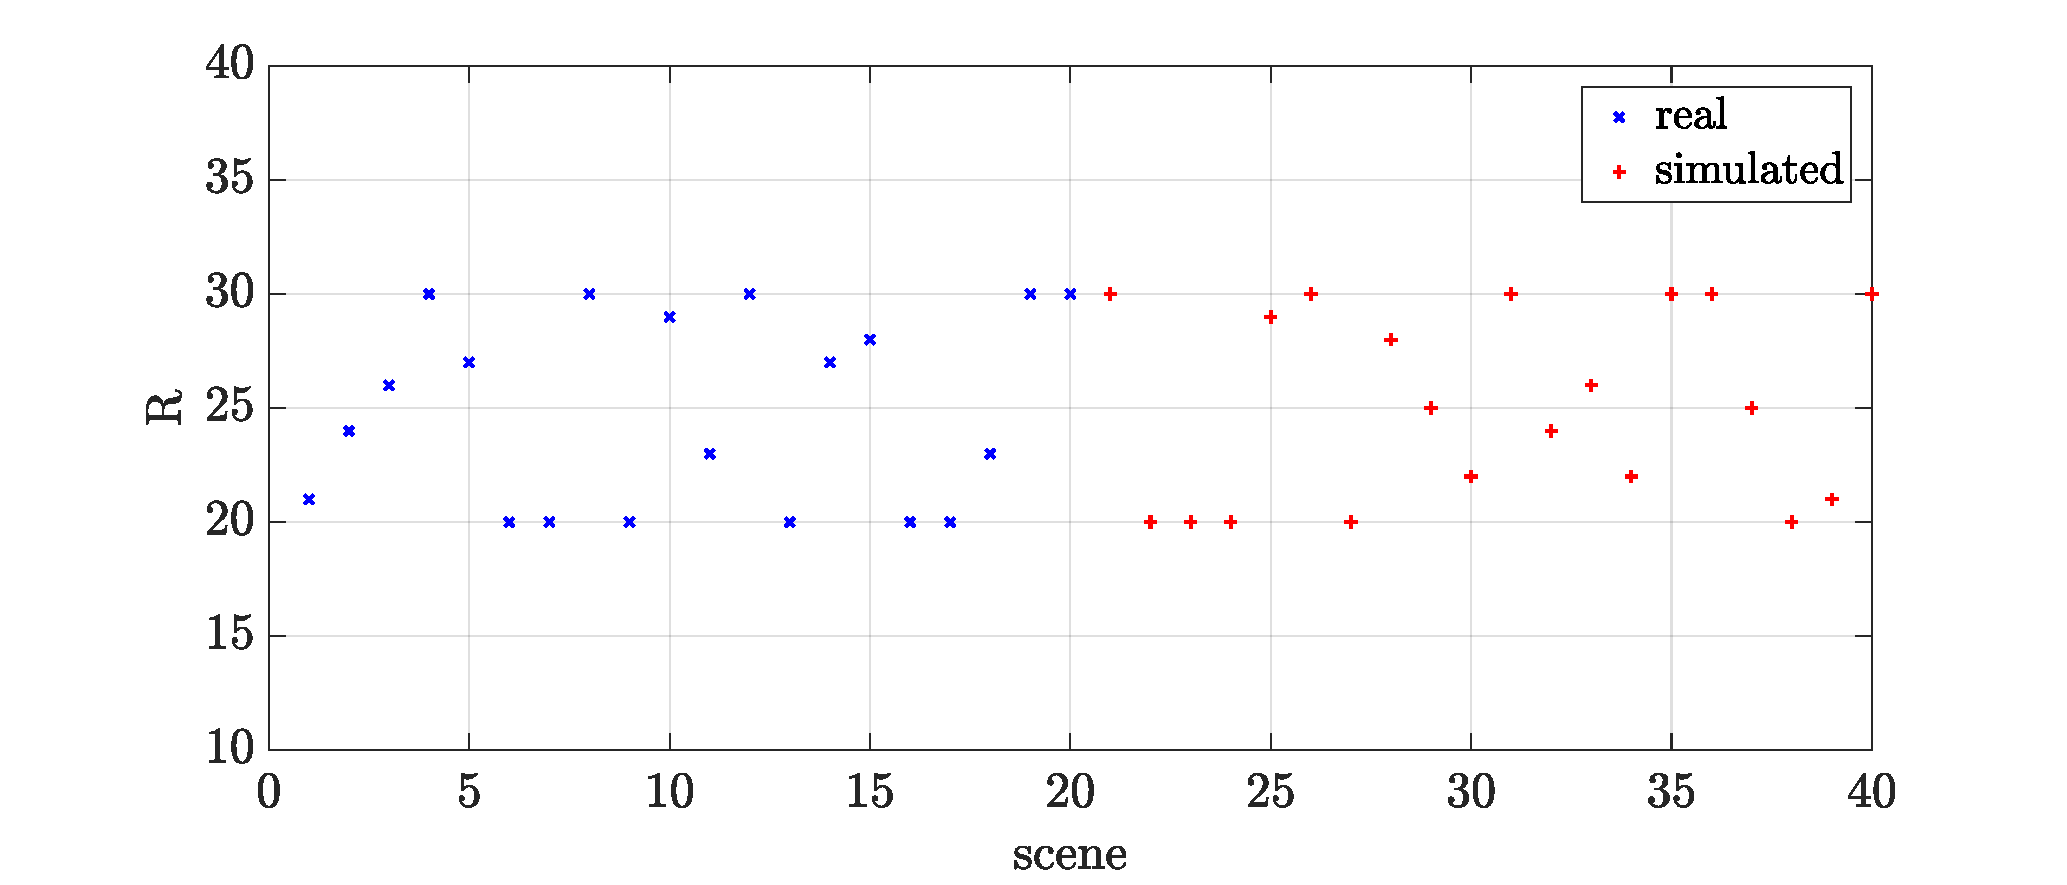
\includegraphics[width = 0.7\textwidth]{./figures/test_perceptif/nb_replication.pdf}
\caption{Nombre de réplication, $R$, pour chaque scène obtenu dans $X_{opt}$ avec comme combinaison $J = 50$, $B = 40$, $K = 20$. Les 20 premières scènes sont les scènes issues des enregistrements du projet GRAFIC, les 20 suivantes sont les scènes répliquées sous \textit{SimScene}.}
\label{fig:replication}
\end{figure}

L'optimisation du plan ne permet alors pas d'avoir un nombre de réplication $R$ constant mais variable évoluant dans l'intervalle $\left[20-30 \right]$ (Figure~\ref{fig:replication}). \\

Une page web \footnote{http://soundthings.org/research/xpRealism} est mis en ligne le 8 février 2017 permettant l'accès au test à un large public et s'est clôturé 12 jours plus tard. Chaque juge écoute donc une succession de 20 extraits audio de 30 secondes dans un ordre établit par le plan optimal. Chaque audio peut être réécouté autant de fois que voulu avant d'être évalué sans qu'il soit toutefois possible de revenir sur son évaluation. L'auditeur a également la possibilité de laisser un commentaire sur chaque audio pour justifier son choix. En fin de test, afin de connaitre le panel d'évaluateur, il leur est demandé de renseigner leur âge, leur sexe (H/F) et leur expérience quant à l'écoute de mixtures sonores urbaines.\\

Les fichiers résultats sont stockés également sous une page web \footnote{http://soundthings.org/research/xpRealism/responses/} et téléchargeable sous le format .json pour ensuite être traités sous le logiciel Matlab.\\

\subsection{Résultats}

L'ensemble des résultats sont soumis à différents tests statistiques afin de comparer les évaluation des scènes enregistrées et répliquées puis pour observer l'influence des différents auditeurs sur l'évaluation ainsi que celle de l'ambiance sonores.

\subsubsection{Constitution du panel}

La Figure \ref{fig:panelTest} résume, sous forme d'histogrammes, l'âge, le sexe et l'expérience des auditeurs. 2 personnes n'ont renseigné aucun de ces champs et une troisième personne a seulement omis de préciser son genre.\\

\begin{figure}[ht]
\centering
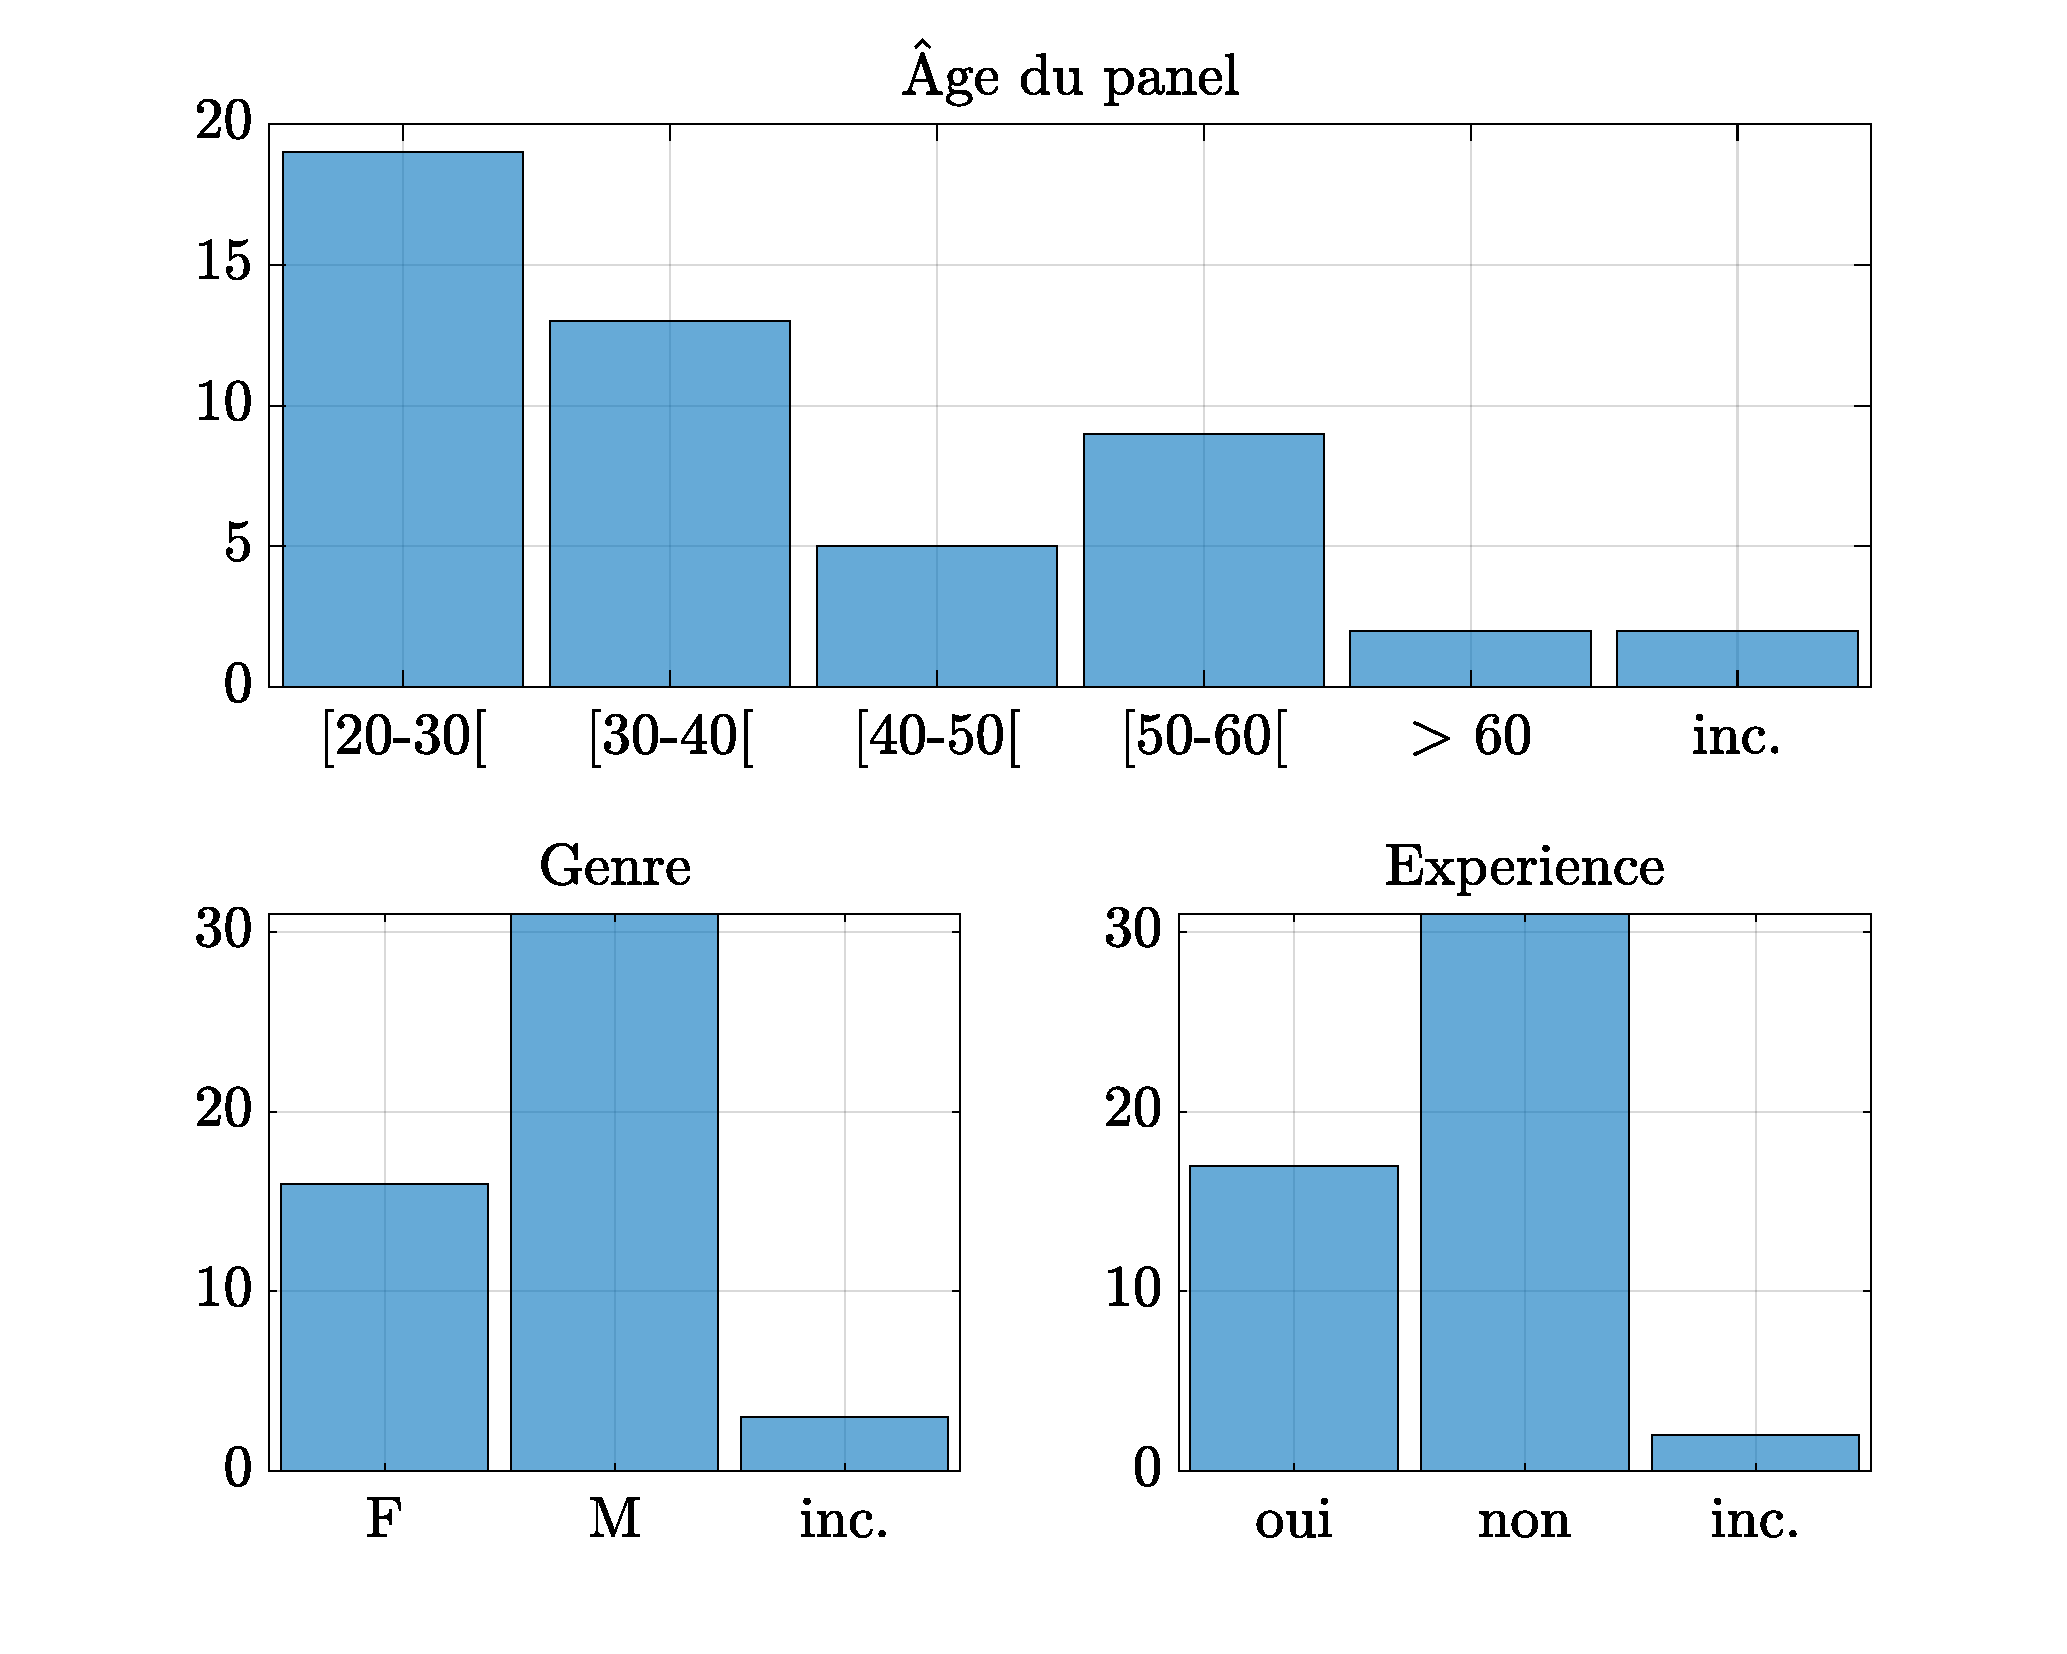
\includegraphics[width = .8\textwidth]{./figures/test_perceptif/testPerceptif_panel.pdf}
\caption{Résumé des informations relatifs aux auditeurs}
\label{fig:panelTest}
\end{figure}

Le panel est composé à 62 $\%$ d'hommes et à 32 $\%$ de femmes. La classe d'âge $\left[20-30\right[$ est la plus représentée suivie de la classe $\left[30-40\right[$ (26 $\%$), $\left[50-60\right[$ (18 $\%$), $\left[40-50\right[$ ($10\%$) et enfin de la classe $>60$ (4 $\%$) . 62 $\%$ du panel a déclaré n'avoir pas d'expérience dans l'écoute d'ambiances sonores urbaines.\\

\subsubsection{Distribution des notes des scènes enregistrées et répliquées} 

Dans un premier temps, la distribution de toutes les notes des scènes enregistrées et répliquées est exprimée au travers d'un schéma en boîte à moustache (Figure \ref{fig:ANOVA_scene}). Cette représentation graphique permet de comparer plusieurs distributions en résumant pour chaque boîte la médiane (trait plein rouge), les valeurs du  premier quartile au troisième quartile (boîte en bleue), la valeur maximale et minimale de la distribution (respectivement trait supérieur et inférieur en noir). \`A cela est également ajoutée la moyenne.\\

\begin{figure}[h]
\centering
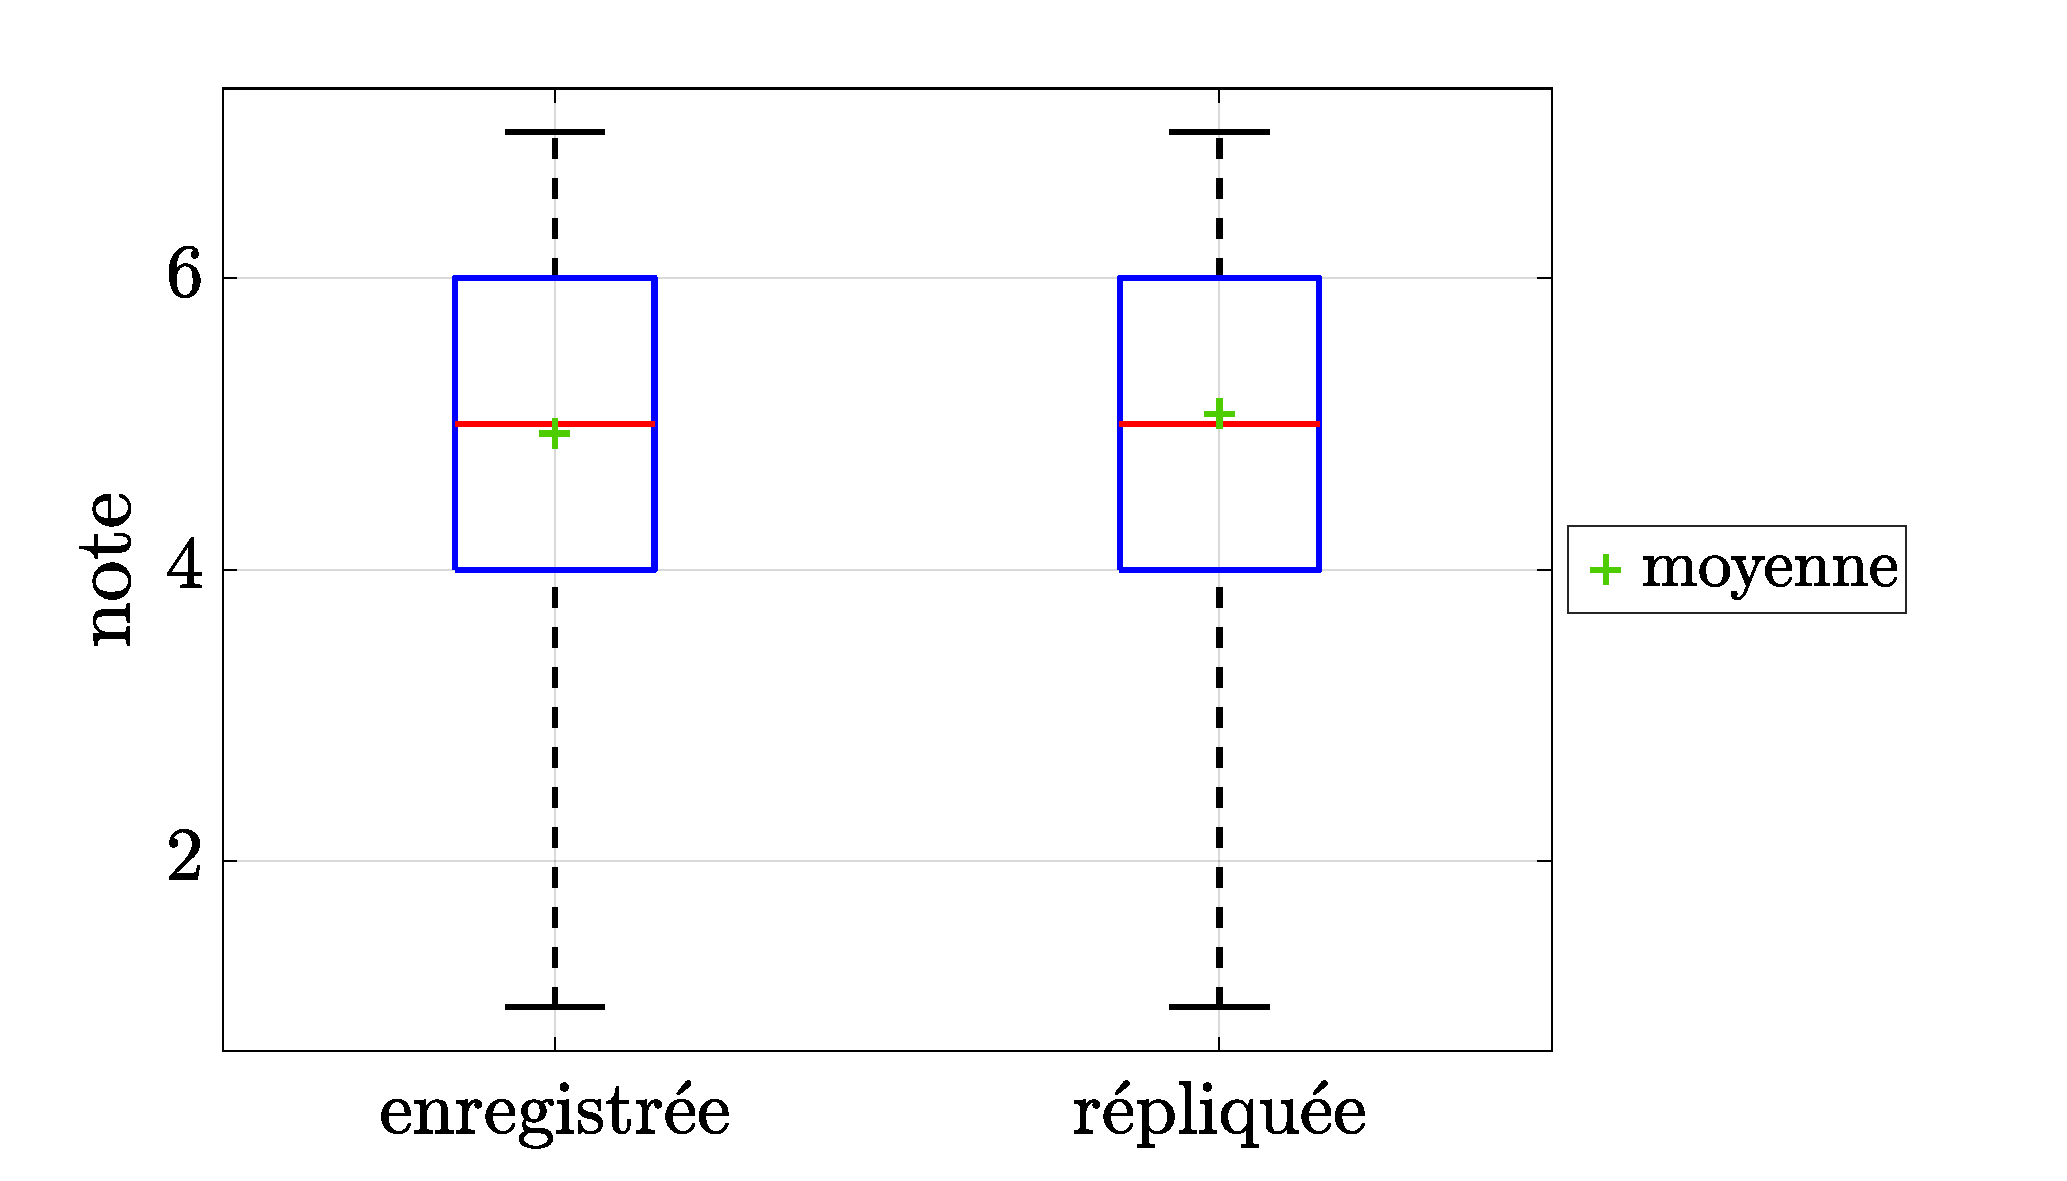
\includegraphics[width = 0.8\textwidth]{./figures/test_perceptif/testPerceptif_boxplotType.pdf}
\caption{Représentation en diagramme en boîte à moustache entre les scènes réelles et simulées}\label{fig:ANOVA_scene}
\end{figure}

La répartition des notes pour les deux types de scènes est fortement similaire. Chaque type présente des valeurs identiques (médiane, valeurs extrêmes, quantiles). Seule la note moyenne permet de différencier les deux ensembles ($m_{En} = 4,93 (\pm 1,64) / 7$ et $m_{Re} = 5,06 (\pm 1,56) / 7$) où la note moyenne des scènes répliquées est légèrement supérieure.\\

À cette première observation, un test $t$ de Student est considéré pour chaque scène entre les notes de la catégorie \textit{enregistrée} et la catégorie \textit{répliquée}. Un test de Student consiste à comparer les moyennes de 2 groupes d'échantillons pour déterminer si elles sont significativement différentes d'un point de vue statistique. Toutefois, puisque pour chaque scène, les évaluations entre le pendant \textit{enregistré} et \textit{répliqué} sont réalisées par des individus différents, que le nombre d'évaluation par catégorie n'est pas identique et que les variances entre les deux catégories ne sont pas égales, c'est une variante du test-$t$ de Student qui est réalisée : le test-$t$ de Welch \cite{ruxton2006unequal}. Dans ce test, pour chaque scène, deux hypothèses sont émises sur les distributions :

\begin{itemize}
\item les distributions des échantillons des deux catégories sont semblables (hypothèse \textit{nulle} $H_0$),
\item les deux distributions sont différentes, (hypothèse \textit{alternative} $H_1$).\\
\end{itemize}

Plusieurs statistiques sont alors définies :
\begin{itemize}
\item la valeur $t$

\begin{equation}
t = \frac{\bar{X}_1-\bar{X}_2}{\sqrt{\frac{s_1^2}{N_1}+\frac{s_2^2}{N_2}}},
\end{equation}

où $\bar{X}_i$, $s_i$ et $N_i$ sont, respectivement, la moyenne de l'échantillon, la variance et le nombre d'échantillon de la catégorie $i$,
\item les degrés de liberté $DDL$

\begin{equation}
DDL = \frac{\left(\frac{s_1^2}{N_1}+\frac{s_2^2}{N_2} \right)^2}{\frac{s_1^4}{N_1^2(N_1-1)}+\frac{s_2^4}{N_2^2(N_2-1)}}
\end{equation}

\end{itemize}

Ces statistiques sont alors utilisées avec une loi de Student pour déterminer une valeur $p$ qui permet de rejeter (ou non) l'hypothèse $H_0$ selon une valeur seuil de référence $\alpha$ (défini à 5 $\%$) :

\begin{itemize}
\item si $\alpha >$ $p$, il existe alors au moins deux distributions différentes, l'hypothèse $H_0$ est rejetée et $H_1$ est acceptée,
\item si $\alpha <$ $p$, l'hypothèse $H_0$ n'est pas considérée comme \textit{vraie} mais on considère qu'il n'y a pas de raison à rejeter $H_0$. Cette nuance provient du fait que cette décision se base sur un nombre limité d'informations (le nombre total d'observations) qui ne permet pas de rejeter totalement l'hypothèse $H_1$.\\
\end{itemize}

Par soucis de concision, seul l'ensemble des 20 valeurs $t$ calculées et les boites à moustaches de chaque scène sont résumés dans les Figures \ref{fig:test-student} et \ref{fig:boxplot_scene}.

\begin{figure}[ht]
\centering
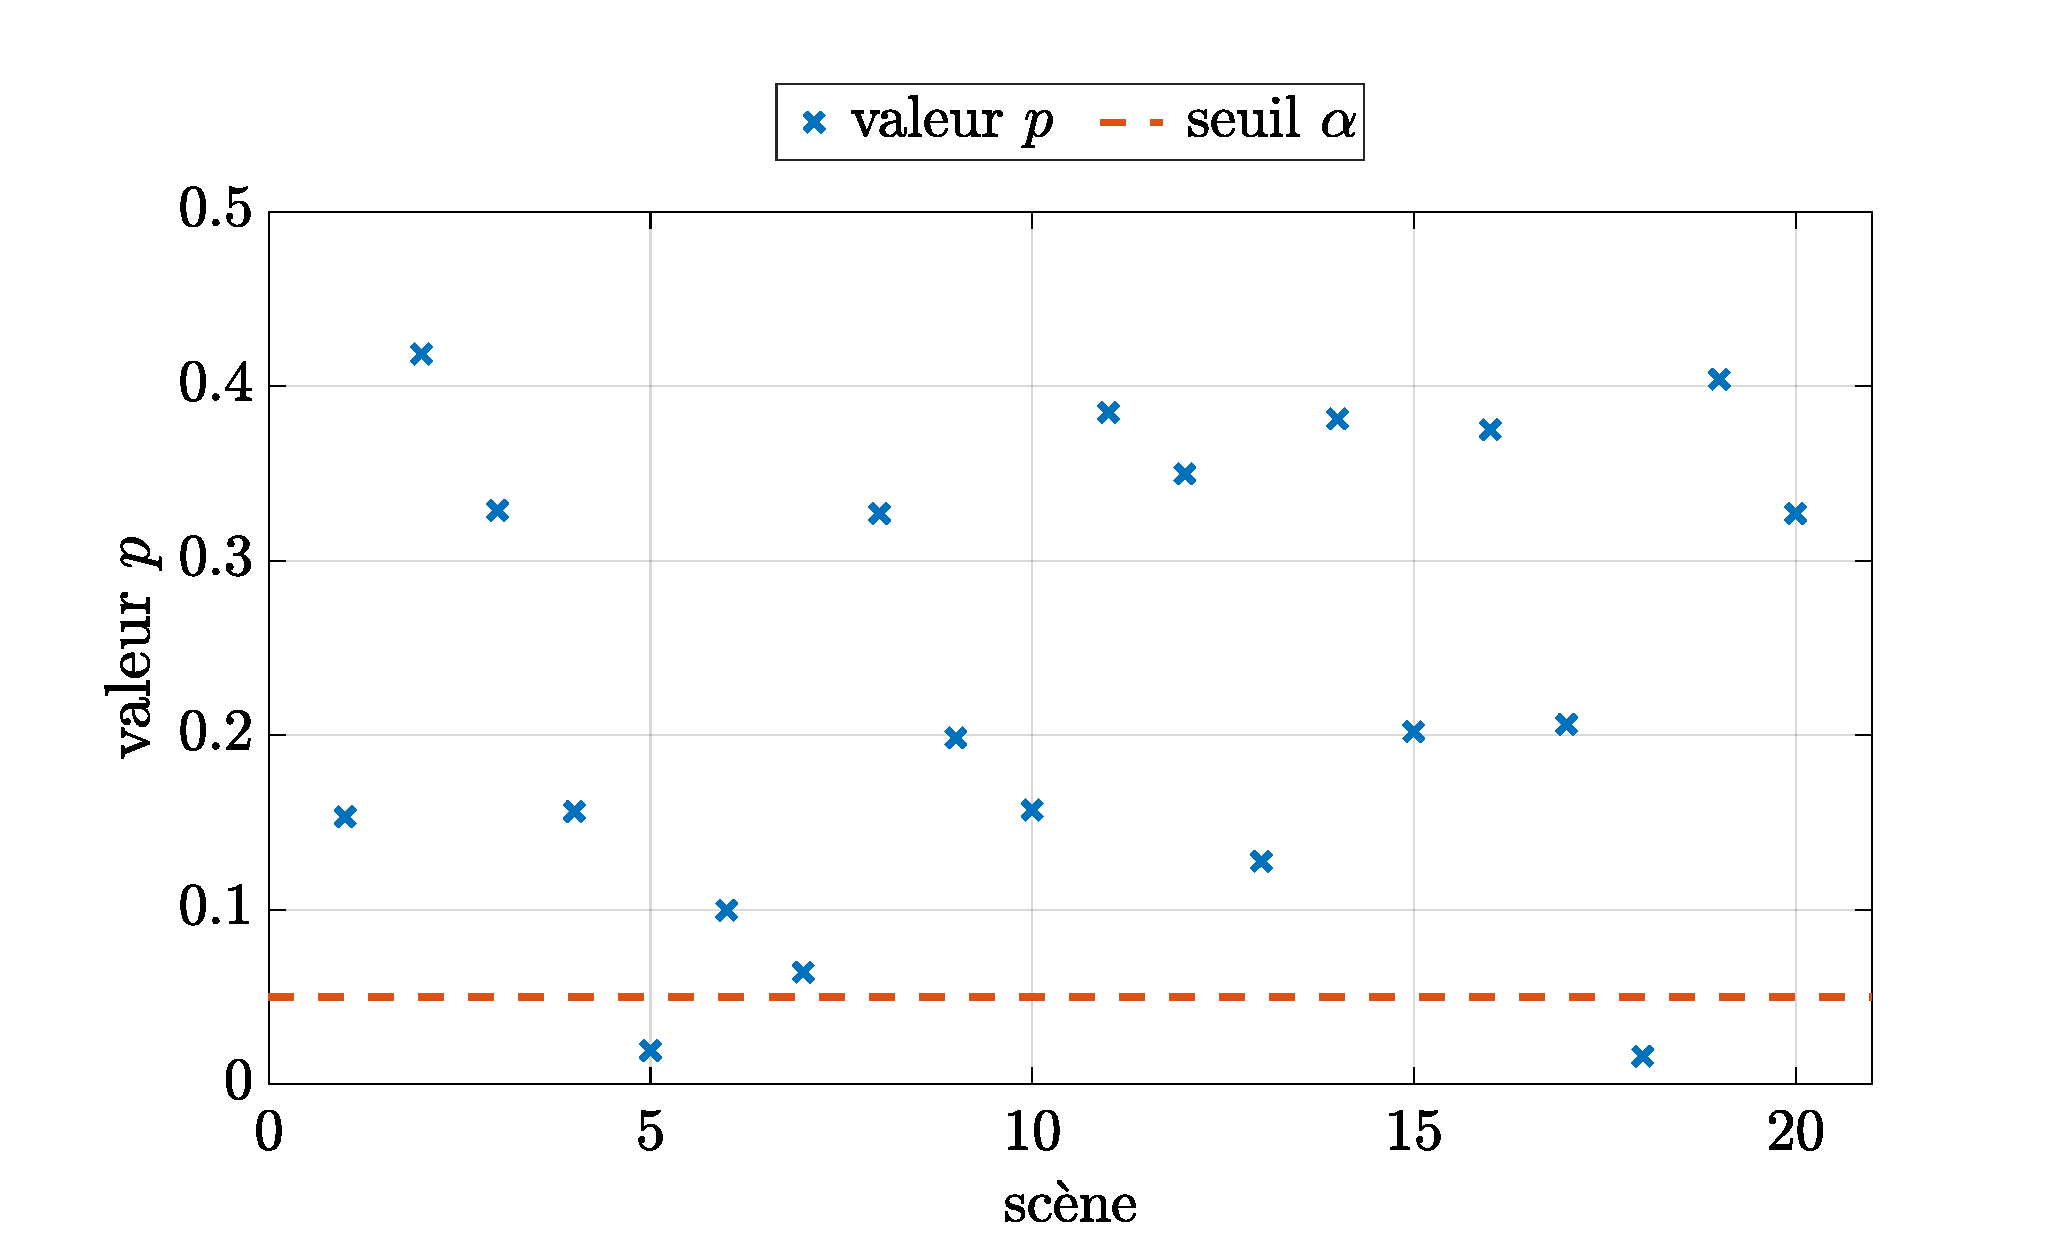
\includegraphics[width = 0.8\textwidth]{./figures/test_perceptif/t-value-student.pdf}
\caption{Résumé des valeurs $p$ calculés pour chaque scène entre les notes issues du type \textit{enregistré} et du type \textit{répliqué}.}\label{fig:test-student}
\end{figure}

\begin{figure}[ht]
\centering
\subfigure[\label{fig:boxplotEnreg}]{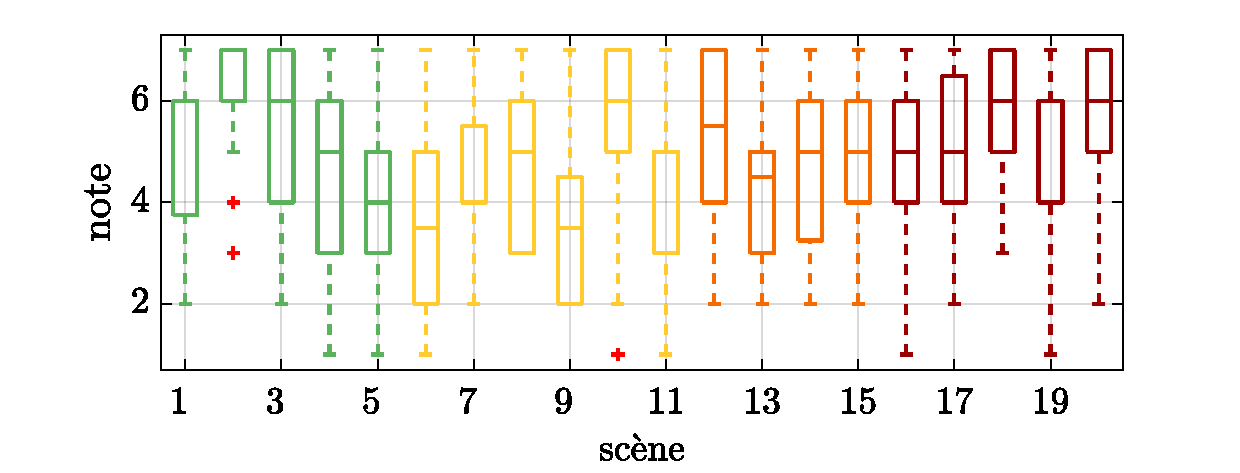
\includegraphics[width=0.7\linewidth]{./figures/test_perceptif/boxplotSceneEnregistree.pdf}}
\subfigure[\label{fig:boxplotRepli}]{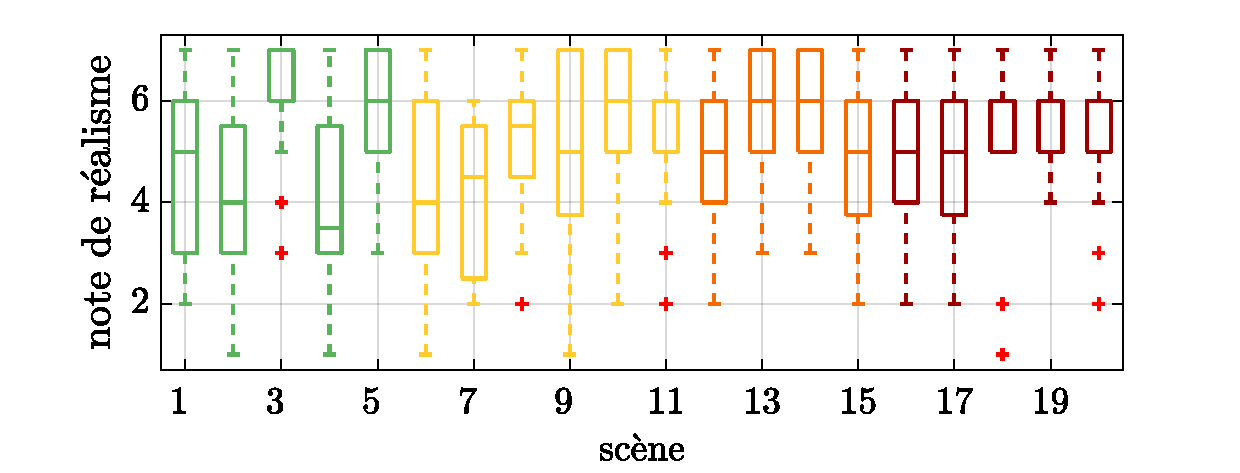
\includegraphics [width=0.7\linewidth]{./figures/test_perceptif/boxplotSceneRepliquee.pdf}}

\begin{tabular}{|p{1.5cm}|l|p{0.001cm}|p{2cm}|l|p{0.001cm}|p{2cm}|l|p{0.001cm}|p{2.75cm}|l|}
\hhline{|-|-|~|-|-|~|-|-|~|-|-|}
Parc & {\cellcolor[HTML]{5AB25A}} & & Rue calme & {\cellcolor[HTML]{FFCB2F}} & & Rue animée & {\cellcolor[HTML]{F56B00}} & &  Rue très animée & {\cellcolor[HTML]{9A0000}}\\
\hhline{|-|-|~|-|-|~|-|-|~|-|-|}
\end{tabular}

\caption{Boites à moustaches pour les scènes enregistrées  \subref{fig:boxplotEnreg} et pour les scènes répliquées \subref{fig:boxplotRepli} classé selon leur ambiance sonore.}

\label{fig:boxplot_scene}
\end{figure}

L'ensemble des tests de Student mené sur les 20 couples de scènes révèlent des valeurs $p$ supérieures au seuil de signification $\alpha$ de 5 $\%$. L'hypothèse $H_0$ n'est donc pas rejetée sur l'ensemble des scènes : le réalisme des scènes testées du type \textit{répliquée} est alors considéré comme similaire à celui du type \textit{enregistrée}.


\subsubsection{Effets des auditeurs sur l'évaluation des scènes}

Pour aller plus loin, une analyse de variance (abrégée ANOVA pour \textit{ANalyse Of VAriance} en anglais) est réalisée afin de déterminer l'influence de chaque auditeur sur l'évaluation des scènes. En effet, selon l'auditeur, l'échelle des notes émises peut varier (un auditeur peut noter sur l'ensemble de l'échelle, d'autres peuvent noter une échelle réduite), influençant l'interprétation des résultats.

C'est ainsi une ANOVA à deux facteurs (\textit{type de scènes} (\textit{enregistré}, \textit{répliqué}) et \textit{auditeur} (50 auditeurs)) avec interaction qui est considérée. De la même manière que le test de Student, l'ANOVA est un outil statistique qui permet de comparer des moyennes d'échantillons et d'étudier l'effet des variables qualitatives (ou facteurs), pouvant prendre plusieurs valeurs (ou niveaux), sur une variable quantitative.
Pour cela, plusieurs statistiques sont calculées (somme des carrés des écarts, le degré de liberté du facteurs, la variance, la statistique de Fischer $F$). De ces indices, la valeur \textit{p} établie, là encore, la probabilité d'obtenir une valeur limite du test si $H_0$ est vraie par rapport à la valeur seuil $\alpha$. Les définitions de ces indices sont résumées en annexe \ref{annexe:}. Les résultats sont résumés dans le Tableau \ref{tab:anova_auditeur}.

\begin{table}[ht]
\centering
\begin{tabular}{lccccc}
\hline
\textbf{Source}     & \textbf{SCE} & \textbf{DDL} & \textbf{variance} & \textbf{F} & \textbf{p-valeur} \\
\hline
\textbf{auditeur} & 687,93 & 49 & 14,03 & 7,89 & <1e-4 \\
\hline
\textbf{type} & 3,61 & 1 & 3,61 & 1,82 & 0,18 \\
\hline
\textbf{auditeur/type} & 93,29 & 49 & 0,90 & 0,55 & 0,55 \\
\hline
\textbf{erreur}      & 1780,42 & 899 & 1,98 & &  \\
\hline
\textbf{total}      & 2572 & 998 & & & \\
\hline
\end{tabular}
\caption{Résultat de l'ANOVA avec interaction avec les facteurs \textit{type} et \textit{auditeur}}
\label{tab:anova_auditeur}
\end{table}

Le facteur \textit{auditeur} a une influence significative (valeur $p$ < $\alpha$) révélant que les auditeurs n'ont pas les même échelle d'évaluation. L'influence du facteur \textit{type} reste toujours non significative. Son interaction avec le facteur \textit{auditeur} est non-significatif également.
Le phénomène d'interaction traduit l'influence des différents niveaux d'un facteur sur l'autre facteur. Ici, l'interaction entre le facteur \textit{auditeur} et \textit{type} est non-significative, ce qui signifie que pour chaque juge, la perception des scènes est similaire, même si entre chaque juge des dissimilarités existent.

\subsubsection{Effets de l'ambiance sonore}

Une seconde ANOVA à deux facteurs avec interaction est effectuée avec pour facteur le \textit{type} (\textit{enregistrée}, \textit{répliquée}) et l'\textit{ambiance sonore} (\textit{parc, rue calme, rue bruyante, rue très bruyante}) afin de déterminer si la perception du réalisme est différent selon l'ambiance sonore. Les résultats de l'ANOVA sont résumés dans le Tableau \ref{tab:anova_ambiance}.

\begin{table}[ht]
\centering
\begin{tabular}{lccccc}
\hline
\textbf{Source}     & \textbf{SCE} & \textbf{DDL} & \textbf{variance} & \textbf{F} & \textbf{p-valeur} \\
\hline
\textbf{type} & 5,72 & 1 & 5,72 & 2,28 & 0,13 \\
\hline
\textbf{ambiance} & 42,65 & 3 & 14,21 & 5,66 & 8,00e-4 \\
\hline
\textbf{type/ambiance} & 36,83 & 3 & 12,27 & 4,89 & 2,20e-3 \\
\hline
\textbf{erreur}      & 2488,49 & 991 & 2,55 & &  \\
\hline
\textbf{total}      & 2572 & 998 & & & \\
\hline
\end{tabular}
\caption{Résultat de l'ANOVA avec interaction avec les facteurs \textit{type} et \textit{ambiance}}
\label{tab:anova_ambiance}
\end{table}


Si l'impact du facteur \textit{type} est toujours non significatif, celui du facteur \textit{ambiance} et l'interaction entre les deux facteurs sont toutefois significatifs ($p < \alpha$). L'influence principale du facteur \textit{ambiance} signifie qu'il y a une distinction entre les distributions des notes selon l'ambiance sonore. Le phénomène d'interaction traduit alors la perception du type de la scène varie suivant pour les différentes ambiances sonores.

Pour visualiser ce phénomène d'interaction entre le type de scènes et l'ambiance sonore, l'évolution de la note moyenne dans chaque cas est tracé (Figure \ref{fig:interaction_ambianceType}). On observe que selon l'ambiance sonore, la note de réalisme des scènes répliquées peut être inférieure ou supérieure par rapport aux scènes enregistrée. Cette évolution traduit une interaction croisée dont l'origine est toutefois difficile à estimer. Il est possible, pour mieux comprendre ces différences, de s'intéresser aux commentaires laissés par les auditeurs sur certaines scènes. Ces derniers relèvent notamment des sons trop forts ou qui s'inscrivent mal dans les scènes (par exemple oiseaux trop fort dans la scène 21, bruit de pas trop fort dans la scène 24). Enfin certains extraits de voix ne sont pas suffisamment réalistes. En effet, lors de la phase d'écoutes des enregistrement, on remarque que les voix perçues, en dehors d'un brouhaha de foule, sont le plus souvent des bribes de conversations de personnes entre elles ou au téléphone. Malheureusement, il n'a pas été possible de trouver des bases de données libres de conversation suffisamment réalistes pour être inclus dans les scènes. De nombreuses bases de données se concentrent, par exemple, sur la lecture de textes récités \cite{el2011survey, kominek2004cmu, barker2015third} ce qui ne permet pas d'atteindre le réalisme souhaité. Les extraits de voix présent dans le corpus élémentaire sont des sons trouvés par défauts, brefs ("hello", "how are you ?") et qui diffèrent beaucoup des voix entendues en ville.

\begin{figure}[h]
\centering
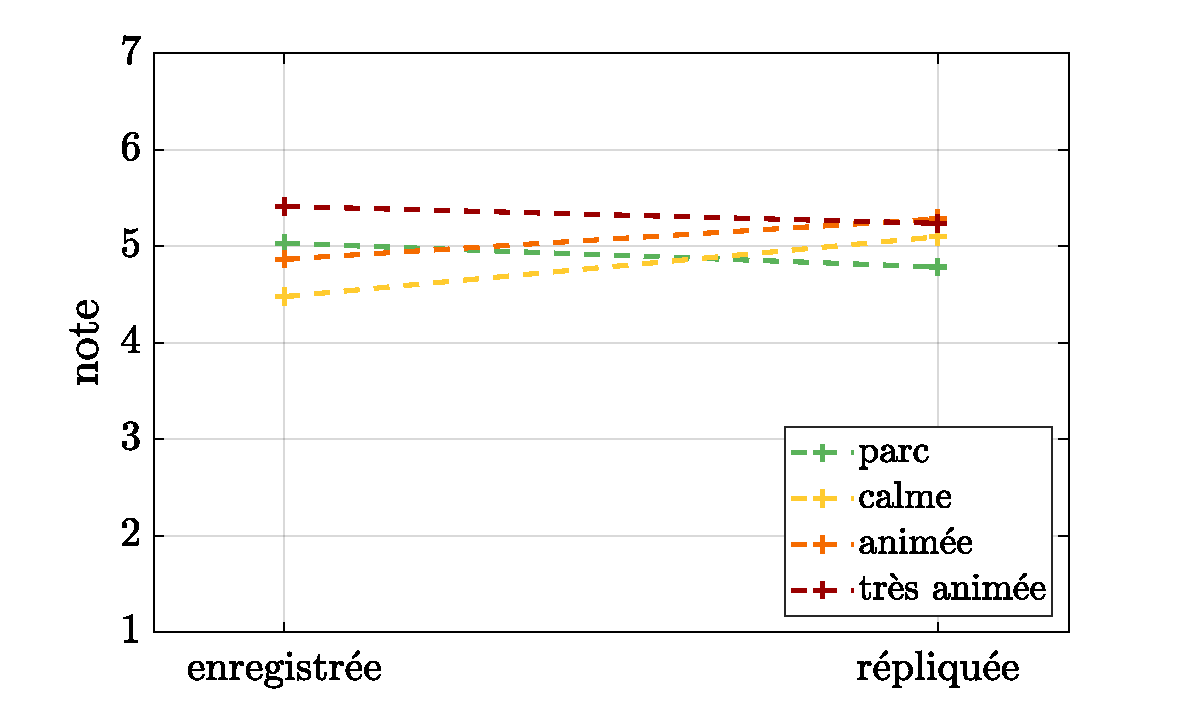
\includegraphics[width=0.8\linewidth]{./figures/test_perceptif/testPerceptif_interactionAmbiance.pdf}
\caption{Évolution de la note moyenne du réalisme par ambiance et selon le type.}\label{fig:interaction_ambianceType}
\end{figure}


Même si les moyennes globales et les distributions entre les scènes enregistrées et répliquées sont similaires, des disparités existent selon les auditeurs ou les ambiances sonores sans toutefois que celles-ci remettent en cause les similarités entre les deux types.\\


En conclusion, sur l'ensemble du corpus testé, il y a donc une similarité du réalisme perçu par l'ensemble des participants entre les scènes enregistrées et répliquées. Même s'il y a des disparités entre les distributions des notes selon les ambiances sonores, l'évaluation du réalisme selon les types de scènes et les ambiances restent similaires (les notes restent comprises entre 4 et 6). 
Certains sons dans les scènes répliquées sembleraient toutefois mal calibrés, ce qui, sur certaines scènes, impacte leur note. Mais on retrouve également ce phénomène dans les scènes réelles, ce qui viendrait à relativiser cette mauvaise calibration.
En conséquence, le réalisme perçu des scènes répliquées est considéré comme similaire à celles des scènes réalistes. 
De ces résultats, comme l'ensemble des scènes répliquées est réalisés avec le même dispositif, on généralise ce résultat à l'ensemble du corpus élémentaire SOUR.\\

Deux corpus de scènes sonores urbaines ont été construits :
\begin{itemize}
\item le corpus d'évaluation \textit{Ambiance} où le trafic est mêlé à une classe de son générique et où le niveau sonore du trafic est calibré.  Ce corpus a pour objectif de tester le comportement de la NMF.
\item le corpus d'évaluation \textit{SOUR} qui est la transcription d'enregistrement sonore urbain en scènes simulées. La réalisation de ces scènes simulées a été soumis à un test perceptif qui a révélé que les scènes simulées étaient perçues de façon similaire à des enregistrements audio. Les conclusions de ce test sont alors étendu à l'ensemble du corpus construit. Ce corpus réaliste a pour vocation à servir l'ensemble des communautés scientifiques développant des outils de reconnaissance, de détection ou de séparation de sources dans un milieu urbain. \\
\end{itemize}

Ces deux corpus sont alors soumis à la NMF afin d'y déterminer quels sont les paramètres qui permettent de déterminer les niveaux sonores \textit{trafic} avec la plus faible erreur.


%Les scènes sont alors créées par un processus en deux parties :
%
%\begin{itemize}
%\item un analyse de phase où des évènements sinusoïdaux, transitoires et le bruit de fond sont séparés d'un enregistrement audio. Les évènements sinusoïdaux sont sélectionnés à partir d'une représentation temps-fréquence du signal. En fixant des fréquences limites et une amplitude seuil, les évènements sont extraits du signal; les régimes transitoires sont extraits à partir des variations d'énergies brusques du signal dans le domaine temporel. Enfin le bruit de fond est le signal résiduel restant après l'extraction des évènements sonores.
%\item Une phase de synthèse où chaque signal extrait est modifié. Pour les sons sinusoïdaux, ces modifications peuvent être fréquentielles, en multipliant les fréquences des spectres par un facteur, ou bien temporelles en changeant sa durée (allongement, troncature...). Les signaux en régime transitoire peuvent être aussi modifiés en hauteur et en durée à l'aide d'un vocoder de phase. Quant au bruit de fond, le choix est fait de générer un nouvel audio similaire à un des audio extraits, à partir d'un algorithme d'apprentissage en arbres d'ondelettes.
%\end{itemize}

%%Ce test statistique considère plusieurs statistiques : un nombre de facteur $F$ comprenant chacun un nombre $N$ de niveaux où $M_n$ observations sont réalisées dans chaque niveau. Le modèle s'exprime alors :
%%
%%\begin{equation}
%%y_{in} = \alpha_i + \beta_j + \gamma_{ij}+\epsilon_{ijk}
%%\end{equation}
%%
%%où $\alpha_i$ et $\beta_j$ sont respectivement les effets des niveaux $i$ et $j$ du 1\er et 2\nd facteur, $\gamma_{ij}$ est l'interaction produite par ces deux facteurs et $\epsilon_{ijk}$ est l'erreur aléatoire qui suit une loi Normale $\mathbb{N}(0,\sigma^2)$.
%%
%%Deux hypothèses sont alors émises sur les distributions :
%%
%%\begin{itemize}
%%\item les distributions des niveaux $n$ et $m$ sont semblables (hypothèse \textit{nulle} $H_0$),
%%\item les deux distributions sont différentes, (hypothèse \textit{alternative} $H_1$).\\
%%\end{itemize}
%%
%%Le test statistique de Fischer détermine alors si l'hypothèse $H_0$ est vraie ou fausse (et donc si l'hypothèse $H_1$ est vérifiée). Ce test consiste à établir le rapport $\mathbf{F}$ de deux variances,
%%
%%\begin{equation}
%%\mathbf{F} = \frac{var_1}{var_2}.
%%\end{equation}
%%
%%Le problème étant à 1 dimension, la variance totale $var_{tot}$ s'exprime comme la somme de la variance du modèle $var_{mod}$ (appelé variabilité inter-niveau) et celui d'un résidu $var_{res}$ (ou variabilité intra-niveau) :
%%
%%\begin{equation}
%%var_{tot} = var_{mod} + var_{res}.
%%\end{equation}
%%
%%En considérant un nombre d'observation total $M = \sum_{k = 1}^{K} M_k$, chacune de ces variances s'exprime comme
%%
%%
%%\begin{equation}
%%var_{mod} = \frac{SCE_{mod}}{DDL_{mod}},
%%\end{equation}
%%
%%\begin{equation}
%%var_{res} = \frac{SCE_{res}}{DDL_{res}}
%%\end{equation}
%%
%%avec
%%
%%\begin{itemize}
%%\item la somme des carrés des écarts du modèle, $SCE_{mod} = \sum_{n=1}^{N} m_n (\bar{y}_{in} - \bar{y})^2$,
%%\item la somme des carrés des écarts du résidu, $SCE_{res} = \sum_{i=1}^{M_n} \sum_{n=1}^{N} (y_{in} - \bar{y}_n)^2$,
%%\item le degré de liberté du modèle, $DDL_{mod} = F-1$,
%%\item le degré de liberté du résidu, $DDL_{res} = M-F$,
%%\item $\bar{y} = $
%%\end{itemize}
%%
%%
%%Le rapport $\mathbf{F}$ s'exprime alors :
%%\begin{align}
%%\mathbf{F} & = \frac{var_{mod}}{var_{res}}\\
%%& = \frac{\nicefrac{SCE_{mod}}{DDL_{mod}}}{\nicefrac{SCE_{res}}{DDL_{res}}}\\
%%& = \frac{M-F}{F-1}\frac{\sum_{n=1}^{N} m_n (\bar{y}_{in} - \bar{y})^2}{\sum_{i=1}^{M_n} \sum_{n=1}^{N} (y_{in} - \bar{y}_k)^2}.
%%\end{align}
%%
%%Des degrés de libertés et de la valeur $\mathbf{F}$, on peut déterminer la \textit{p-valeur} (à l'aide des tables de Fischer ou à l'aide de logiciels comme \textit{R} ou Matlab) qui établit la probabilité d'obtenir une valeur limite du test si $H_0$ est vraie. Cette valeur est comparée a une seuil de signification $\alpha = 0.05$.
%
%
%
%\subsubsection{Par type de scènes}
%
%Dans le cas du test perceptif, on considère un seul facteur ($F = 1$), le réalisme de la scènes, qui comprend deux niveaux \textit{réelles} et \textit{simulées} ($N = 2$), chaque niveaux ayant un nombre d'observation $M_n$ correspondant à l'ensemble des notes du panel appartenant à l'un des deux niveaux et un nombre totale d'individu $M = J \times K = 1000$. Une ANOVA est réalisée sous le logiciel Matlab et les résultats sont résumés dans le tableau \ref{tab:anova}.\\
%
%\begin{table}[ht]
%\centering
%\begin{tabular}{lccccc}
%\hline
%\textbf{Source}     & \textbf{SCE} & \textbf{DDL} & \textbf{variance} & \textbf{F} & \textbf{p-valeur} \\
%\hline
%\textbf{réalisme} & 4.62         & 1            & 4.62              & 1.79       & 0.18              \\
%\hline
%\textbf{erreur}      & 2567.40      & 997          & 2.57              &            &                   \\
%\hline
%\textbf{total}      & 2572.00         & 998          &                   &            &       \\
%\hline
%\end{tabular}
%\caption{Résultat de l'ANOVA calculé}
%\label{tab:anova}
%\end{table}
%
%
%La \textit{p-valeur} est supérieure au seuil de signification $\alpha$ et est supérieur à 0.1. Il n'y a donc pas de présomption contre l'hypothèse $H_0$. On peut alors considéré qu'il n'y a pas de distinction possible entre les scènes simulées et réelles faites par le panel. \\
%
%En plus des résultats textuels, une représentation graphique sous forme de diagramme en boîte à moustache est faite selon le type de scènes (figure \ref{fig:ANOVA_scene}). Cette représentation graphique permet de comparer plusieurs distributions en résumant pour chaque boîte la médiane (trait plein rouge), les valeurs du  premier quartile au troisième quartile (boîte en bleue), la valeur maximale et minimale de la distribution (respectivement trait supérieur et inférieur en noir). \`A cela est également ajoutée la moyenne.\\
%
%\begin{figure}[h]
%\centering
%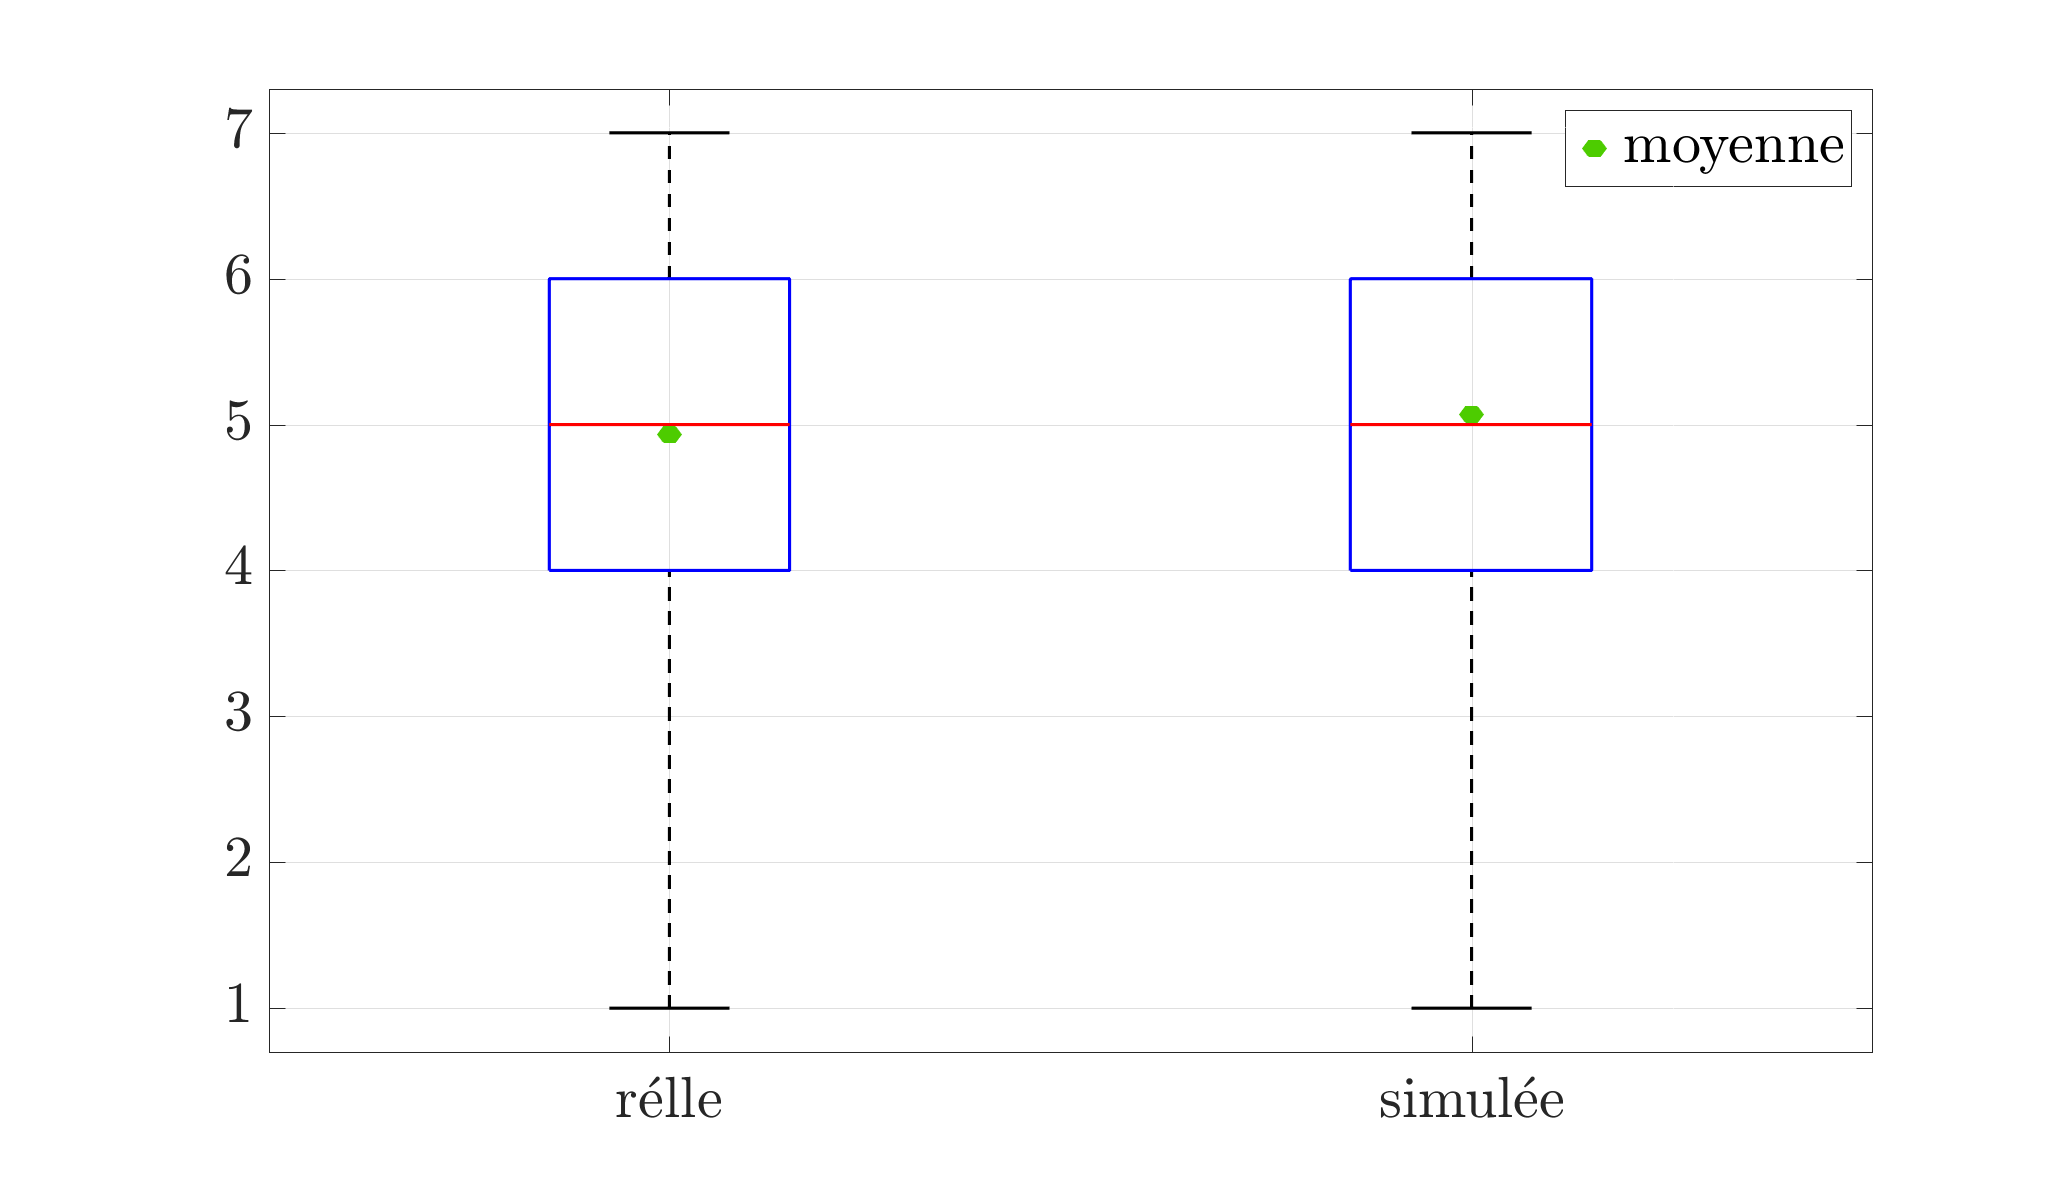
\includegraphics[width = 0.8\textwidth]{./figures/test_perceptif/testPerceptif_boxplotType_FR.png}
%\caption{Représentation en diagramme en boîte à moustache entre les scènes réelles et simulées}\label{fig:ANOVA_scene}
%\end{figure}
%
%La répartition des notes pour les deux type de scènes, quelque soit l'expérience de l'auditeur, est similaire. Chaque type présente des valeurs identiques (médiane, valeurs extrêmes, quantiles). Seule la note moyenne permet de différencier les deux ensembles : $m_{Re} = 4.93 \pm 1.64$ et $m_{Si} = 5.06 \pm 1.56$. Les deux valeurs sont quasiment similaires confirmant que les deux distributions sont donc bien identiques et que les scènes simulées ont un rendu similaire aux enregistrements réels. \\
%
%\subsubsection{Par expérience et par type de scènes}
%Il est possible de déterminer l'influence de l'expérience de l'auditeur dans les écoutes d'ambiances urbaines dans l'évaluation des scènes par un ANOVA (tableau~\ref{tab:anova_exp}, figure~\ref{fig:ANOVA_exp}). Il y a donc ici 2 facteurs $F$, le type de scènes et l'expérience, qui ont 2 niveaux $N$ chacun (respectivement Re/Si et expérience/sans expérience).
%
%\begin{table}[ht]
%\centering
%\begin{tabular}{lccccc}
%\hline
%\textbf{Source}     & \textbf{SCE} & \textbf{DDL} & \textbf{variance} & \textbf{F} & \textbf{p-valeur} \\
%\hline
%\textbf{réalisme} & 4.62         & 1            & 4.62              & 1.79       & 0.18              \\
%\hline
%\textbf{expérience}    & 4.85         & 1            & 4.85              & 1.89       & 0.16              \\
%\hline
%\textbf{erreur}      & 2562.52      & 997          & 2.57              &            &                   \\
%\hline
%\textbf{total}      & 2572.00         & 999          &                   &            &       \\
%\hline
%\end{tabular}
%\caption{Résultat de l'ANOVA calculé}
%\label{tab:anova_exp}
%\end{table}
%
%\begin{figure}[h]
%\centering
%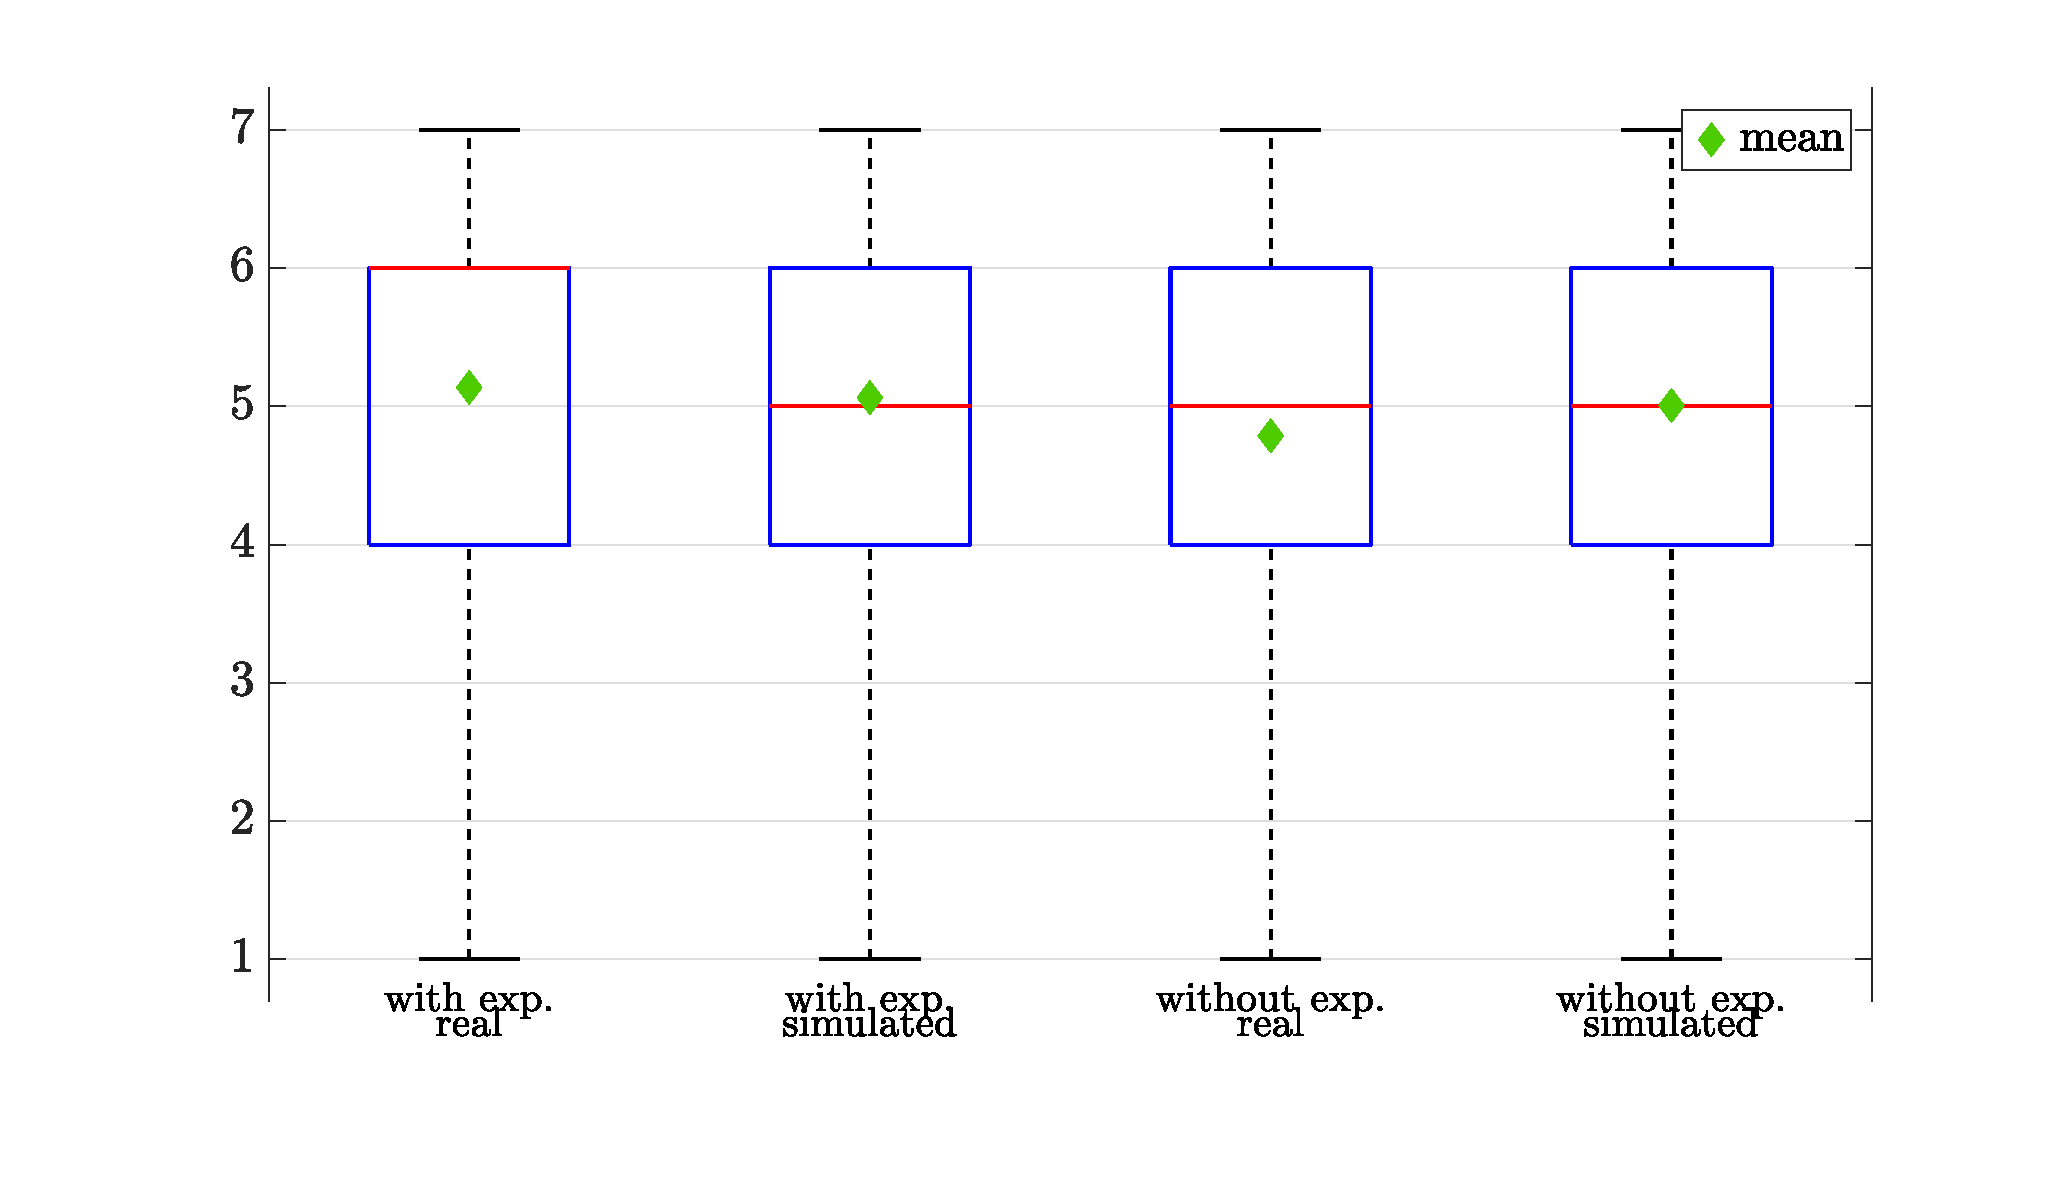
\includegraphics[width = 0.8\textwidth]{./figures/test_perceptif/testPerceptif_boxplotExperience_EN.pdf}
%\caption{Distribution des notes selon le type de scène et l'expérience dans l'écoute des scènes sonores urbaines}\label{fig:ANOVA_exp}
%\end{figure}
%
%
%\begin{table}[]
%\centering
%\begin{tabular}{p{3cm} C{3cm} C{3cm}}
%\cline{2-3}
% & \multicolumn{2}{c}{\textbf{type}} \\
%\cline{2-3}
% & \textbf{réelle} &  \textbf{simulée} \\ \hline
%\textbf{avec expérience} &  $5.13 \pm 1.60$ & $5.06 \pm 1.70 $ \\ \hline
%\textbf{sans expérience} &  $4.83 \pm 1.65$ & $5.07 \pm 1.49$ \\ \hline
%\end{tabular}
%\caption{Moyennes obtenue selon l'expérience et le type de scènes}
%\label{my-label}
%\end{table}
%
%Si on différencie les auditeurs selon leur expérience dans l'écoute d'ambiances sonores urbaines, on constate que les auditeurs expérimentés évalue mieux les scènes réelles que les scènes simulées à l'inverse des auditeurs sans expériences. De plus, si les moyennes pour les scènes simulées sont fortement similaires quelque soit l'expérience, la notation des scènes réelles est différente. Des retours et remarques faites par plusieurs panéliste permette de supposer que les auditeurs plus expérimentés sont plus susceptibles de faire attention aux détails de la scènes (composition des évènements sonores, connaissance sur la panel de sons pouvant être présents, différence de réverbération entre les sources sonores..) rendant les scènes simulées plus identifiables. À l'opposé, les auditeurs non expérimentés vont plus s'attarder à évaluer l'ensemble de la scène. Or comme les scènes simulées sont constitué de sons qui sons isolés initialement, il est plus facile pour l'auditeur de les reconnaitre dans la scène qu'il écoute et donc de se \og  projeter \fg{} dans le milieu urbain. Dans certaines scènes réelles, les sources sonores étant moins discernables la perception du réalisme est réduite.\\
%
%Toutefois, malgré ces faibles différences, les moyennes et les distributions restent, là encore, similaires et permettent de conclure que même avec de l'expérience dans l'écoute de scènes urbaine, la qualité des audio simulées est satisfaisante.\\
%
%\subsubsection{Par ambiance et par scène}
%
%On regroupe, dans la figure~\ref{fig:boxplot_ambiance}, les scènes par ambiances sonores (\textit{parc}, rue \textit{calme}, rue \textit{animée}, rue \textit{très animée}).\\
%
%\begin{figure}[hbtp]
%\centering
%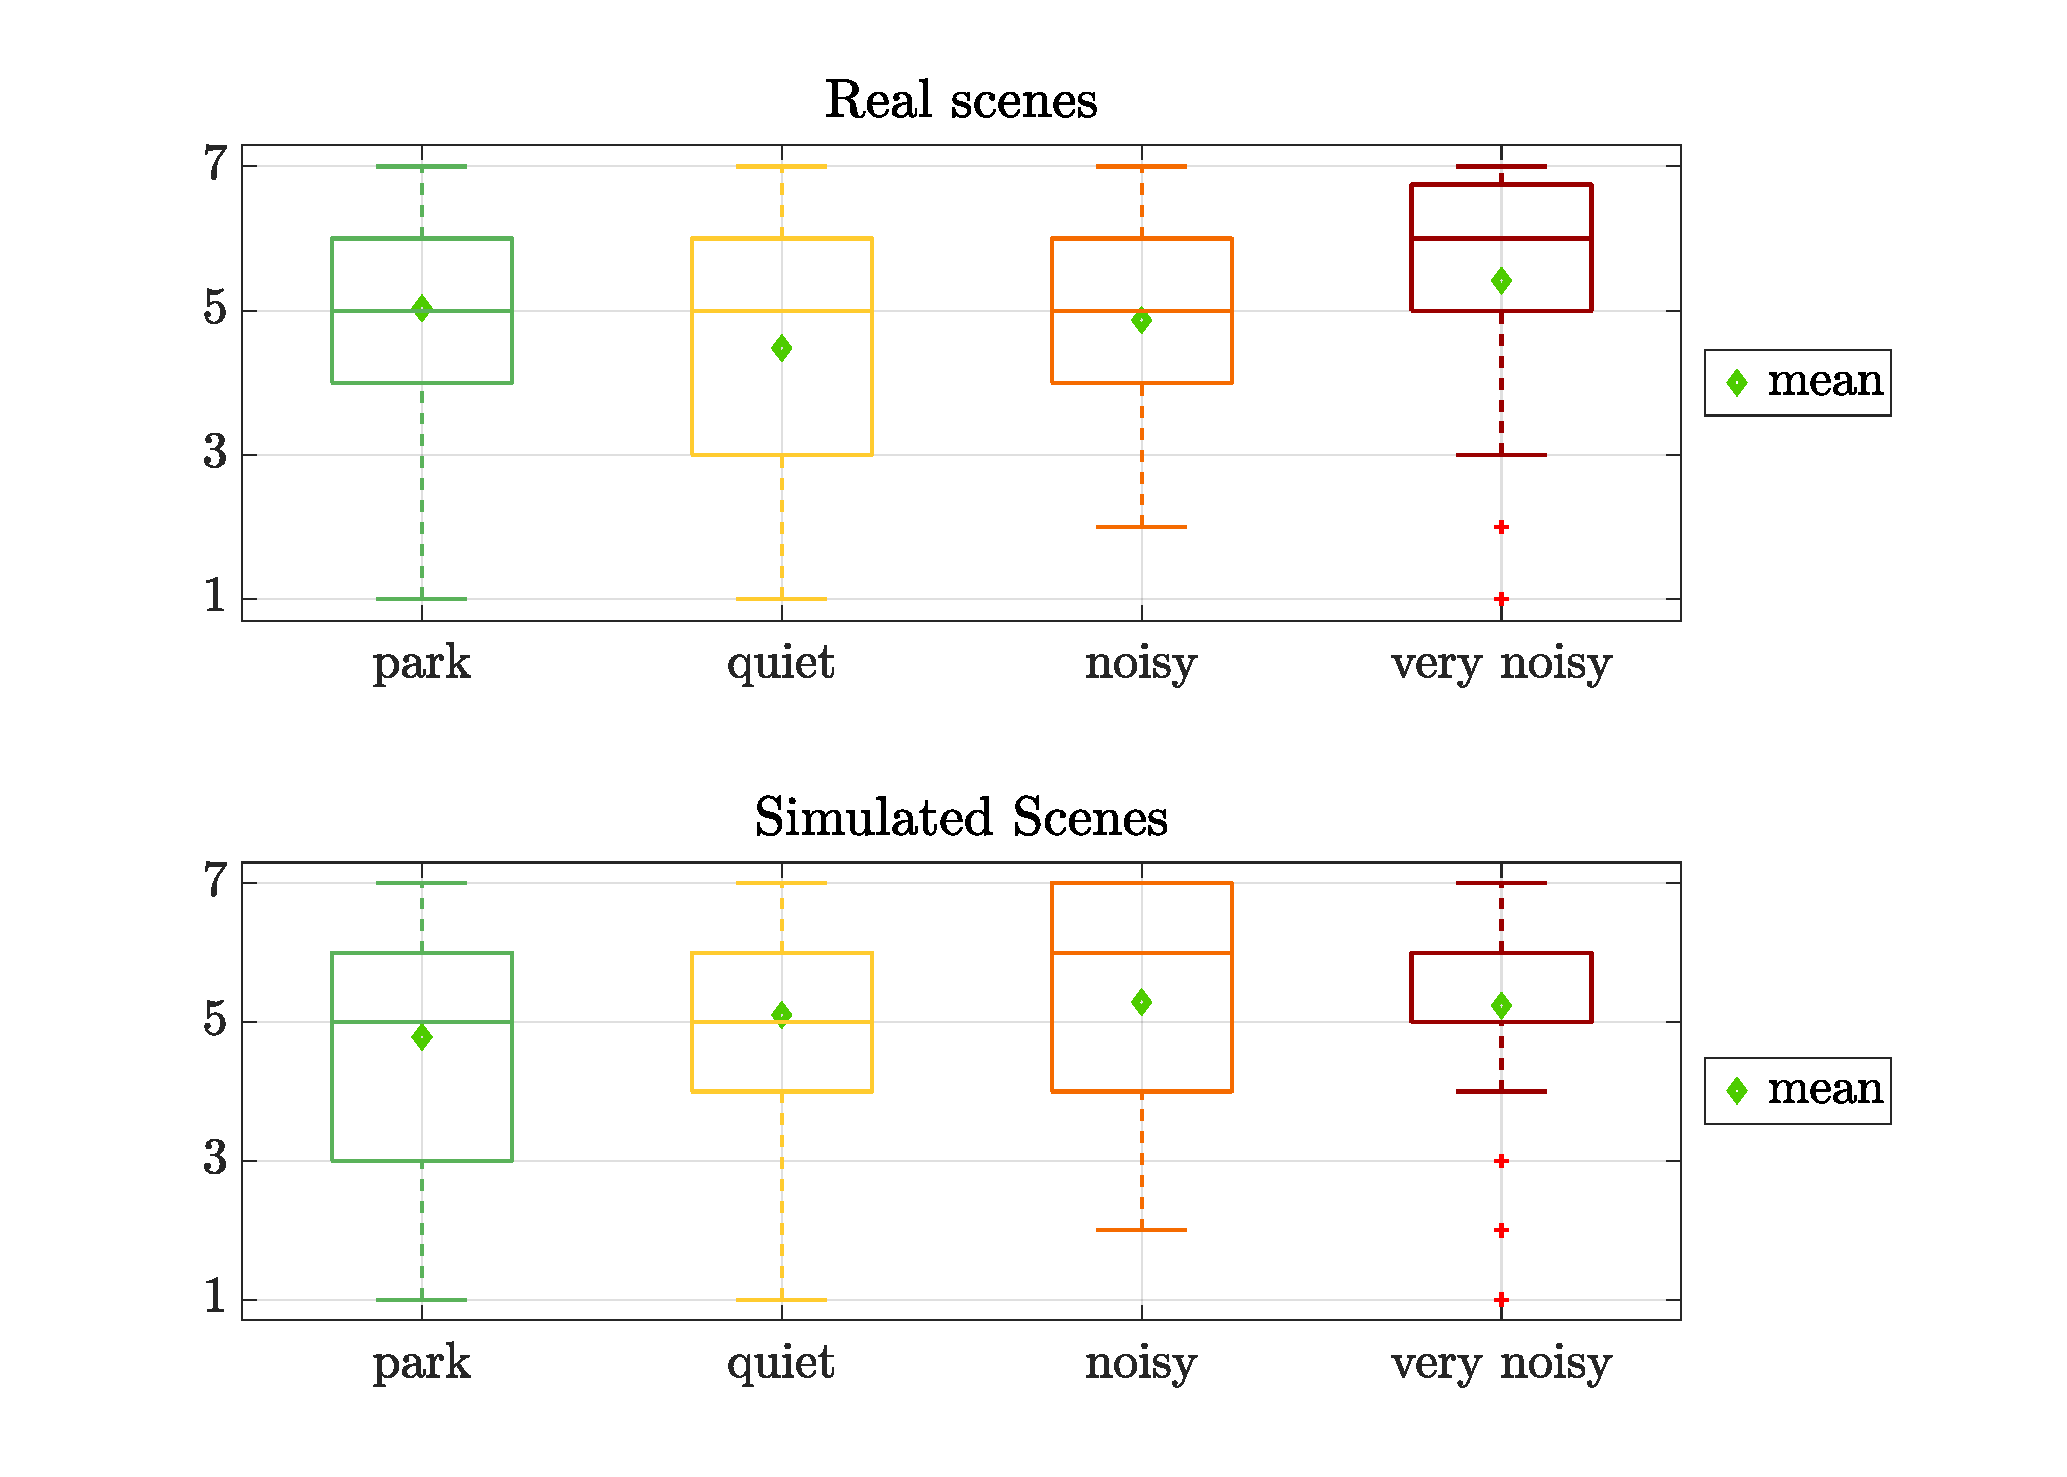
\includegraphics[width=0.7\textwidth]{./figures/test_perceptif/testPerceptif_boxplotAmbianceCOLOR_EN.pdf}
%
%\begin{tabular}{|p{1.5cm}|l|p{0.001cm}|p{2cm}|l|p{0.001cm}|p{2cm}|l|p{0.001cm}|p{2.75cm}|l|}
%\hhline{|-|-|~|-|-|~|-|-|~|-|-|}
%Parc & {\cellcolor[HTML]{5AB25A}} & & Rue calme & {\cellcolor[HTML]{FFCB2F}} & & Rue animée & {\cellcolor[HTML]{F56B00}} & &  Rue très animée & {\cellcolor[HTML]{9A0000}}\\
%\hhline{|-|-|~|-|-|~|-|-|~|-|-|}
%\end{tabular}
%
%\caption{Distribution en fonction de l'ambiance sonore pour les scènes réelles (en haut) et les scènes simulées (en bas)}
%\label{fig:boxplot_ambiance}
%\end{figure}
%
%
%Cette représentation permet de constater que les ambiances sonores \textit{animée} et \textit{très animée}, dans les deux types de scènes, sont évaluées comme les plus réalistes : la médiane et la moyenne sont élevées avec une distribution peu dispersée. \`A l'inverse, les ambiances plus calmes (\textit{parc} et \textit{calme}) sont plus dispersés et ont une note moyenne plus faible. C'est donc les ambiances constituées en majorité du trafic qui sont les mieux évalués. Les scènes dans les parcs et rues calmes, constituées de moins de trafic et plus de sons urbains divers (voix, bruit de pas, oiseaux), sont moins bien évaluées aussi bien pour les scènes issus d'enregistrements que celles créer.\\
%
%Enfin, pour chaque scène, la distribution des notes est établie et sont mis en relation avec les commentaires laissés par les auditeurs (figure~\ref{fig:ANOVA_scene}).\\
%
%\begin{figure}[h]
%\centering
%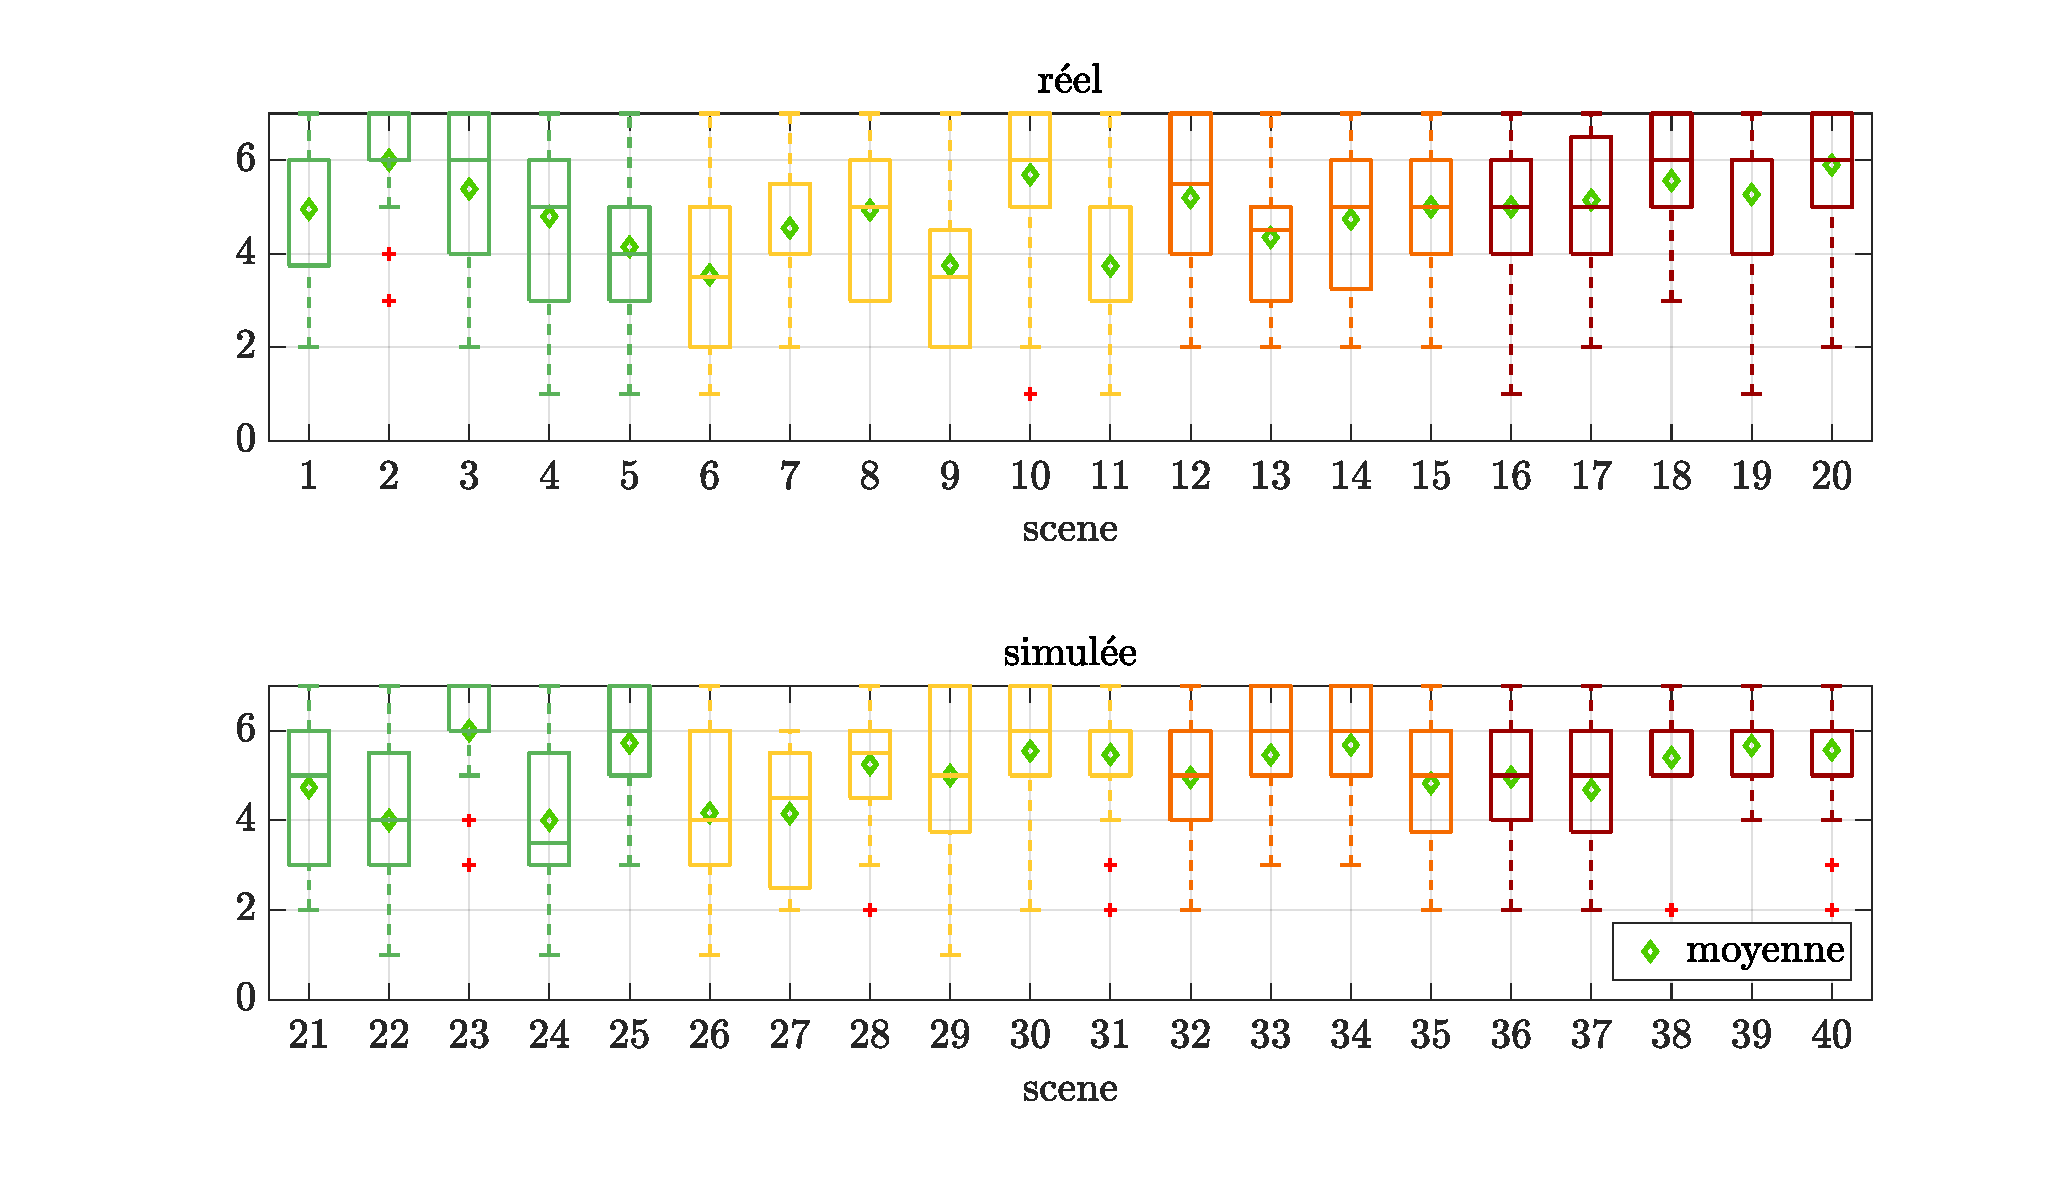
\includegraphics[width=.9\textwidth]{./figures/test_perceptif/testPerceptif_meanPerSceneCOLOR.pdf}
%
%\begin{tabular}{|p{1.5cm}|l|p{0.001cm}|p{2cm}|l|p{0.001cm}|p{2cm}|l|p{0.001cm}|p{2.75cm}|l|}
%\hhline{|-|-|~|-|-|~|-|-|~|-|-|}
%Parc & {\cellcolor[HTML]{5AB25A}} & & Rue calme & {\cellcolor[HTML]{FFCB2F}} & & Rue animée & {\cellcolor[HTML]{F56B00}} & &  Rue très animée & {\cellcolor[HTML]{9A0000}}\\
%\hhline{|-|-|~|-|-|~|-|-|~|-|-|}
%\end{tabular}
%
%\caption{Distribution par scène pour les scènes réelles (de 1 à 20) et les scènes simulées (de 21 à 40)}
%\label{fig:moyParScene}
%\end{figure}
%
%
%Plusieurs observations peuvent être émises :
%\begin{itemize}
%\item La meilleure moyenne est obtenue pour 2 scènes ex-æquo : la scène 2 (6.0 $\pm$ 1.0) et 23 (6.0 $\pm$ 1.1).
%\item La plus mauvaise moyenne est réalisée pour la scène 6 (3.6 $\pm$ 1.6). C'est donc une scène issu d'un enregistrement qui a été jugé la moins réaliste. Celle-ci a la particularité de n'avoir aucun évènement sonore discernable.
%\item Parmi les 20 scènes simulées, on peut observé 4 scènes dont les moyennes sont plus faibles que les autres (scènes 22, 24, 26 et 27). Dans les scènes 24 et 26, les auditeurs ont remarqué que la présence des bruits de pas paraissent trop fort cassant le réalisme du reste de la scène. La scène 22 est, quant à elle, évaluée plus faiblement en raison d'un bruit de portail également trop fort au début de l'extrait. Ces trois scènes appartiennent à l'ambiance \textit{Parc}. La scène 27 enfin n'a pas reçu de commentaire mais sa note moyenne plus faible peut s'expliquer par un bruit de fond composé d'un nombre d'oiseaux peut être trop grand et qui parait peu réaliste dans un milieu urbain.\\
%\end{itemize}
%
%L'ensemble de cette étude met en évidence les performances de l'outil de simulation qui permet de reconstruire des mixtures sonores urbaines perçues comme suffisamment réalistes. Pour ce test, la réalisation des scènes aux ambiances rue \textit{animée} et \textit{très animée} est très correcte. Les ambiances \textit{parc} et rue \textit{calme} restent bien évalué sur leur réalisme mais sont perfectibles notamment sur certains évènements sonores, non reliés au trafic, qui détériore l'aspect réaliste des scènes. A noter, que les passages de voitures isolés ou la reconstitution du trafic n'ont pas fait l'objet de commentaire.

%Cette méthode établit dans un premier temps, le nombre de combinaison total possible ($J \times B$) puis un premier plan des combinaisons possibles (appelé $X$ de dimension $J \times K$) est élaboré de façon aléatoire. Celui-ci est ensuite mis à jour itérativement en remplaçant chaque combinaison possible $\tau_{j,k}$ par une autre combinaison $\tau^{*}_{j,b}$ extrait de la matrice de combinaison totale, de telle façon à minimiser le produit matriciel \ref{eq:mini_det_BIE}. Ce procédé est le principe de l'algorithme d'échange.

%\begin{equation}\label{eq:mini_det_BIE}
%\underset{\tau_{j,b}}{\text{min}} \det(X'X)^{-1}.
%\end{equation}
%
%Cet algorithme est dit $D$-optimal car il fait intervenir l'opérateur \textit{Déterminant} mais il peut être $A$-optimal en faisant appel à l'opérateur \textit{Trace} à la place. Le résultat est alors un plan $X_{opt}$ de dimensions $J \times K$ résumant l'ordre d'écoutes des fichiers audio pour chaque juge. La Figure \ref{fig:replication} résume le nombre de réplication de chaque scène dans le plan obtenu.\\

%\bibliographystyle{unsrt}
%\bibliography{../bibliographie}
%
%\end{document}
